
\documentclass[11pt,openright,twoside,letterpaper,onecolumn]{report} %% USE THIS FOR DOUBLE SIDED
%\documentclass[11pt,openright,oneside,letterpaper,onecolumn]{report}  %% USE THIS FOR SINGLE SIDED

\usepackage{breakcites}
\usepackage{microtype}
\usepackage{epsfig,endnotes,times}
\usepackage{amsmath}
\usepackage[noend]{algpseudocode}
\usepackage{paralist,algorithm}
\usepackage{booktabs}
%\usepackage{subcaption}
\usepackage{multirow}
\usepackage{float}
\usepackage{graphicx}
\usepackage{pgfplots}

\usepackage{amssymb}
%\usepackage{epstopdf}
%\usepackage{tikz}
%\usepackage{tkz-tab}
\usepackage{xspace}
%\usepackage{epsfig}
%\epstopdfsetup{outdir=./}
%\usepackage[showframe=true]{geometry}
\usepackage{enumitem}
\usepackage{adjustbox}
\usepackage[most]{tcolorbox}

\pgfplotsset{compat=1.10}

\newcommand{\iprobe}{\texttt{iProbe}\xspace}
\newcommand{\docker}{\emph{Docker}\xspace}
\newcommand{\parikshan}{\emph{Kensa}\xspace}
\newcommand{\livedebugging}{\textit{live debugging}\xspace}
%\newcommand{\debugcontainer}{\textit{debug container}\xspace}
\newcommand{\productioncontainer}{\textit{production container}\xspace}
\newcommand{\fio}{\textit{fio}\xspace}
\newcommand{\toolNameLang}{\emph{japanese}\xspace}
%\newcommand{\comment}[1]{}
\newtheorem{example}{Example}
\def\infinity{\rotatebox{90}{8}}

% Complex \xxx for making notes of things to do.  Use \xxx{...} for general
% notes, and \xxx[who]{...} if you want to blame someone in particular.
% Puts text in brackets and in bold font, and normally adds a marginpar
% with the text ``xxx'' so that it is easy to find.  On the other hand, if
% the comment is in a minipage, figure, or caption, the xxx goes in the text,
% because marginpars are not possible in these situations.
{\makeatletter
 \gdef\xxxmark{%
   \expandafter\ifx\csname @mpargs\endcsname\relax % in minipage?
     \expandafter\ifx\csname @captype\endcsname\relax % in figure/caption?
       \marginpar{\textcolor{red}{xxx~}}% not in a caption or minipage, can use marginpar
     \else
       \textcolor{red}{xxx~}% notice trailing space
     \fi
   \else
     \textcolor{red}{xxx~}% notice trailing space
   \fi}
 \gdef\xxx{\@ifnextchar[\xxx@lab\xxx@nolab}
 \long\gdef\xxx@lab[#1]#2{{\bf [\xxxmark \textcolor{red}{#2} ---{\sc #1}]}}
 \long\gdef\xxx@nolab#1{{\bf [\xxxmark \textcolor{red}{#1}]}}
 % This turns them off:
 \long\gdef\xxx@lab[#1]#2{}\long\gdef\xxx@nolab#1{}%
}

%Blue
{\makeatletter
 \gdef\yyymark{%
   \expandafter\ifx\csname @mpargs\endcsname\relax % in minipage?
     \expandafter\ifx\csname @captype\endcsname\relax % in figure/caption?
       \marginpar{\textcolor{blue}{yyy~}}% not in a caption or minipage, can use marginpar
     \else
       \textcolor{blue}{yyy~}% notice trailing space
     \fi
   \else
     \textcolor{blue}{yyy~}% notice trailing space
   \fi}
 \gdef\yyy{\@ifnextchar[\yyy@lab\yyy@nolab}
 \long\gdef\yyy@lab[#1]#2{{\bf [\yyymark \textcolor{blue}{#2} ---{\sc #1}]}}
 \long\gdef\yyy@nolab#1{{\bf [\yyymark \textcolor{blue}{#1}]}}
 % This turns them off:
 \long\gdef\yyy@lab[#1]#2{}\long\gdef\yyy@nolab#1{}%
}

\input{header}

\begin{document}

% For the first pages we do not have numbering 
\pagestyle{empty}

\pdfbookmark{Title}{Title}
\thesistitlepage

\pdfbookmark{Copyright}{Copyright}
\thesiscopyrightpage

\pdfbookmark{Abstract}{Abstract}
\thesisabstract

% In the "roman-numbered" section of the thesis, we have numbers at the bottom
% and we have to reduce the textheight of the text to make space for the number

\pagenumbering{roman}
\pagestyle{plain}

\setlength{\footskip}{0.5in}

\setcounter{tocdepth}{2}
\renewcommand{\contentsname}{Table of Contents}
\pdfbookmark{Table of Contents}{Table of Contents}
\tableofcontents
\cleardoublepage

\listoffigures
\cleardoublepage

\listoftables 
\cleardoublepage

%%%
%%% Acknowledgments
%%%
~\\[1in] % hack to put space at top.
\textbf{\Huge Acknowledgments}\\

\noindent 
First and foremost I would like to acknowledge
\\
I would also like to thank
\\
The work described here has been supported by the Programming Systems Laboratory, and several members of the PSL lab
\\
Last but not the least - 

\cleardoublepage

%%%
%%% Dedication page
%%%
\thispagestyle{plain}
\strut \vfill
{
\centering\LARGE{ 
To my parents, and my sister for their unwavering support, 
and to my wife for her constant encouragement and the final push.
}
}
\vfill \strut
\cleardoublepage

%\draft   % Generates a draft version in single-space

%%%
%%% BODY
%%%
\pagestyle{headings}
\pagenumbering{arabic}

%
% In the "arabic" section of the thesis, we do not have numbers at  the
% bottom and we want to use the full length of the page to avoid vbox
% underfulls. We use the fancyheaders package to adapt the headers
% according to the  Columbia requirements.
%
\setlength{\textheight}{8.5in}
\setlength{\footskip}{0in}

% We change the pagestyle 

% make this true at the time of distrbiution
\fancypagestyle{plain} {%
\fancyhf{}
\fancyhead[LE,RO]{\thepage}
\fancyhead[RE,LO]{\itshape \leftmark}
\renewcommand{\headrulewidth}{0pt}
}
\pagestyle{plain}

\chapter{Introduction}
\label{sec:intro}

%Motivation: What is the problem we are trying to solve? Why does it exist? Why is it important to the community?
Although software bugs are nothing new, the complexities of virtualized environments coupled with large distributed systems have made bug localization harder.
The large size of distributed systems means that any downtime has significant financial penalties for all parties involved.
Hence, it is increasingly important to localize and fix bugs in a very short period of time.

%What is the specific problem considered in this work? This paragraph narrows down the topic area of the work. In the first paragraph you have established general context and importance. Here you establish specific context and background.

%In this work, we show that ...". This is the key paragraph in the intro - you summarize, in one paragraph, what are the main contributions of your work given the context you have established in paragraphs 1 and 2. What is the general approach taken? Why are the specific results significant? This paragraph must be really really good. If you can't "sell" your work at a high level in a paragraph in the intro, then you are in trouble. As a reader or reviewer, this is the paragraph that I always look for, and read very carefully.
%You should think about how to structure this one or two paragraph summary of what your work is all about. If there are two or three main results, then you might consider itemizing them with bullets or in test (e.g., "First, ..."). If the results fall broadly into two categories, you can bring out that distinction here. For example, "Our results are both theoretical and applied in nature. (two sentences follow, one each on theory and application)"

%At a high level what are the differences in what you are doing, and what others have done? Keep this at a high level, you can refer to a future section where specific details and differences will be given. But it is important for the reader to know at a high level, what is new about this work compared to other work in the area.

%The remainder of this work is structured as follows..." Give the reader a roadmap for the rest of the work. Avoid redundant phrasing, "In Section 2, In section 3, ... In Section 4, ... " etc.



%Why do existing techniques not solve this problem
Existing state-of-art techniques for monitoring production systems~\cite{dtrace,winetw,systemtap} rely on light-weight dynamic instrumentation to capture execution traces.
Operators then feed these traces to analytic tools~\cite{magpie,clue} to connect logs in these traces and find the root-cause of the error.
However, dynamic instrumentation has a trade-off between granularity of tracing and the performance overhead.
Operators keep instrumentation granularity low, to avoid higher overheads in the production environment.
This often leads to multiple iterations between the debugger and the operator, to increase instrumentation in specific modules, in order to diagnose the root-cause of the bug.
Another body of work has looked into record-and-replay~\cite{odr,revirt,laadan2010transparent,geels2007friday} systems which capture the log of the system, in order to faithfully replay the trace in an offline environment.
Replay systems try and capture system level information, user-input, as well as all possible sources of non-determinism, to allow for in-depth \textit{post-facto} analysis of the error.
However, owing to the amount of instrumentation required, record-and-replay tools deal with an even heavier overhead, making them impractical for real-world production systems.


%Our approach and story - iprobe first then parikshan
The high level goal of this thesis is to present tools and techniques which can help to reduce the time to bug localization, and can be applied in live running production service systems. 
Our initial efforts focused on having the minimum possible instrumentation in the production system, which could at the same time be dynamically turned on or off. 
We developed \iprobe (see chapter~\ref{ch:iprobe}) an intelligent instrumentation tool, which combined the advantages of static instrumentation and dynamic instrumentation to give an order of magnitude better performance in terms of overhead compared to existing state-of-art tools~\cite{dtrace,systemtap,dyninst,pin}.
\iprobe uses placeholders added in the application binary at compile time, which can be leveraged to insert instrumentation when the application is actually running.
In comparison, most current tools use trampoline based techniques (see DTrace~\cite{dtrace}, SystemTap~\cite{systemtap}, Dyninst~\cite{dyninst}), or just in time execution (PIN~\cite{pin}, Valgrind~\cite{valgrind}), requiring complex operations to allow for safe execution and incurs a much higher overhead.
Our compilation driven place-holders allow us to leverage pre-existing space in the binary to safely insert instrumentation and achieve a much better performance.

However, in the process of our experiments we realized one critical limitation of instrumentation based techniques - instrumentation and monitoring is always done within the code, and hence is sequentially executed. 
Since instrumentation will always directly impact the performance of production applications, it needs to be limited to allow for good user experience.
A better way to approach this problem is to ~\emph{decouple debugging instrumentation and application performance}, so that there is no direct impact of the instrumentation on the production application.
This thesis is centered around the idea of a new debugging paradigm called \emph{``live debugging''}, whereby developers can debug/instrument the application while isolating the impact of this instrumentation from the user-facing production application.
The key idea behind this approach is to give faster time-to-bug localization, deeper insight into the health and activity within the system, and to allow operators to dynamically debug applications without fear of changing application behavior.
We leverage existing work in live migration and light-weight user-space container virtualization, to provide an end-to-end workflow for debugging.
Our system replicates the application container into a clone which can be used solely for the purpose of debugging the application.

%observations which led to the design of \parikshan
Our work is inspired by three key observation: 
Firstly, we observe that most service-oriented applications(SOA) are launched on cloud based infrastructures.
These applications use virtualization to share physical resources, maintained by third-party vendors like Amazon EC2~\cite{ec2}, or Google compute~\cite{gcompute} platforms.
Furthermore, there is an increasing trend towards light-weight user-space container virtualization, which is less resource hungry, and makes sharing physical resources easier.
Frameworks like docker~\cite{docker} allow for scaled out application deployment, by allowing each application service instance to be launched in it's own container.
For instance, an application server, and a database server making up a web-service, can be hosted on their own containers, thereby sandboxing each service, and making it easier to scale out.

Secondly, we observe a trend towards Dev-ops~\cite{devops} by the software engineering industry.
DevOps stresses on close coupling between software developers and operators, in order to have shorter release cycles (Facebook web has 2 releases a day, and one mobile release every 4 weeks and Flickr has 10 deployment cycles per day~\cite{releaseFacebookKeynote,10DevOps}).
This re-emphasizes the need to have a very short time to diagnose and fix a bug especially in service oriented application.
We believe by providing a means to observe the application when the bug is active, we will significantly reduce the time to bug localization.

Lastly, our key insight is that for most service-oriented applications (SOA), a failure can be reproduced simply by replaying the network inputs passed on to the application.
For these failures, capturing very low-level sources of non-determinism (e.g. thread scheduling or general system calls, often with high overhead) is unnecessary to successfully and automatically reproduce the buggy execution in a development environment. 
We have evaluated this insight by studying 16 real-world bugs, which we were able to trigger by only duplicating and replaying network packets.
Furthermore we categorized 220 bugs from three real-world applications, finding that most were similar in nature to the 16 that were reproduced, suggesting that our approach would be applicable to them as well.
\xxx{Please look at section so and so for further details regarding the above}

%contributions
\noindent This thesis will make the following contributions:

First, in Chapter~\ref{ch:parikshan} we will present a framework for ``live debugging'' applications while they are running in the production environment.
This will involve a description of our system called \parikshan\footnote{\parikshan is the Sanskrit word for  testing}, which allows \textbf{real-time debugging} without any impact on the production service.
We provide a facility to sandbox the production and debug environments so that any modifications in the debug environment do not impact user-facing operations.
\parikshan avoids the need of large test-clusters, and can target specific sections of a large scale distributed application.
In particular, \parikshan allows debuggers to apply debugging techniques with deeper granularity instrumentation, and profiling without worrying that the instrumentation will impact the production application performance.

In chapter~\ref{ch:NetworkReplaySurvey} we will present details of our case-study presenting real-world bugs which were triggered by network input alone, and which show why using \parikshan would be enough to capture most real-world bugs. 
Each case study presents a different variety of bugs from the following classes: performance, semantic, non-deterministic, configuration and resource leak. 
We believe that these bugs form the most common classification of bugs in service oriented applications.

In chapter~\ref{ch:iprobe} we will present a dynamic instrumentation mechanism called \iprobe.
%, which can assist developers in making applications \parikshan ready.
As explained earlier, chronologically \iprobe was our first tool developed towards achieving the goal of a low-overhead production debugging.
iProbe uses a novel two-stage design, and offloads much of the dynamic instrumentation complexity to an offline compilation stage.
It leverages standard compiler flags to introduce ``place-holders" for hooks in the program executable.
Then it utilizes an efficient user-space ``HotPatching'' mechanism which modifies the functions to be traced and enables execution of instrumented code in a safe and secure manner.
\iprobe can be used as a standalone instrumentation tool or can be used in the \debugcontainer with \parikshan for further assisting the debugger to localize the bug.

In the final chapter~\ref{ch:activedebugging} of this thesis we focus on applications of live debuggging. 
In particular we discuss several existing techniques and how they can be coupled with live debugging. 
We discuss step-by-step scenarios where debugging on the fly can be helpful, and how it can be applied.
We also briefly introduce a new technique called budget limited instrumentation technique for live debugging.
This technique leverages existing work on statistical debugging, and queuing theory to lay a statistical foundation for allocating buffer sizes and various configuration parameters.
It proposes a reactive mechanism to adapt to the overhead of instrumentation bounds using sampling techniques.

%Secondly, we introduce the concept of active debugging.
%This allows for debuggers to add a patch/or a fix in the debug-container and check if it fixes the error. 
%Similarly tests can be performed while ensuring the production container output is not changed, and forward progress is ensured.
%We isolate tests in \debugcontainer to ensure forward progress, and no impact on the production-container.

The rest of this chapter is organized as follows.
Firstly in section~\ref{sec:introDefinition} we define terms and terminologies used in the rest of this thesis.
Section~\ref{sec:introProblemStatement} further defines the scope of our problem statement, definitions, and classifications of the bugs.
Section~\ref{sec:introRequirements} illustrates the requirements this thesis must meet.
Next, in section~\ref{sec:introScope} we define the scope of the techniques presented in this thesis.
Section~\ref{sec:introApproach} briefly goes over the proposed approach presented in this thesis.
In section~\ref{sec:introHypothesis} we give the hypothesis of this thesis.
Section~\ref{sec:introAssumptions} lists some of the assumptions made in this thesis, and section~\ref{sec:introOutline} gives an outline of the organization of the rest of this document.

\section{Definitions}
\label{sec:introDefinition}

Before we further discuss the problem statement, requirements, and approach,this section first formalizes some of the terms used throughout this thesis.

\begin{itemize}
	
	\item \hypertarget{defn:livedebugging}{\textbf{Live Debugging}}
	For the purpose of this thesis, we define \emph{live debugging} as a mechanism to debug applications on the fly while the production services are running and serving end-users.
	
	\item The \hypertarget{defn:development-environment}{\textbf{development environment}} refers to a setting (physical location, group of human developers, development tools, and production and test facilities) in which software is created and tested by software developers and is not made available to end users.
	The debugging process in the development environment can be interactive, and can have a high overhead.
	
	\item A \hypertarget{defn:production-environment}{\textbf{production environment}}, or use environment, refers to a setting in which software is no longer being modified by software developers and is being actively being used by users.
	Applications in production cannot have a high instrumentation/debugging overhead, as it is detrimental to the users.
	
	\item An \hypertarget{defn:error}{\textbf{error}}, also referred to as a defect or bug, is the deviation of system external state from correct service state.
	
	\item A \hypertarget{defn:fault}{\textbf{fault}} is the adjudged or hypothesized cause of an error.
	
	\item A \hypertarget{defn:failure}{\textbf{failure}} is an event that occurs when the delivered functionality deviates from correct functionality.
	A service fails either because it does not comply with the functional specification, or because this specification did not adequately describe the system function.
	
	\item \hypertarget{defn:devops}{\textbf{DevOps}} is a software development method that stresses communication, collaboration (information sharing and web service usage), integration, automation and measurement of cooperation between software developers and other information-technology (IT) professionals.
	DevOps acknowledges the interdependence of software development and IT operations.
	It aims to help an organization rapidly produce software products and services and to improve operations performance quality assurance.
	
	
	\item \hypertarget{defn:development-phase}{\textbf{Development/Operational Phase}} Development phase is the phase where the application is being developed.
	The process involves testing, and debugging and iterative development such as adding bug fixes etc. Operational phase is where the application is being operated and used by active users
	
	\item \hypertarget{defn:downstream-servers}{\textbf{Downstream Servers}} 
	For a given application or service, the downstream server is the server which sends it a request.
	
	\item \hypertarget{defn:upstream-servers}{\textbf{Upstream Servers}}
	For a given application or service, the upstream servers are servers which process it's requests and send it responses.
	
	
	\item \hypertarget{defn:production container}{\textbf{Production Container}}
	This is the container in which the original production service is hosted and where all incoming requests are routed.
	
	\item \hypertarget{defn:debug container}{\textbf{Debug Container}}
	This is a replica of the production container, where a copy of the production service is running. The debug container is used for debugging purposes, and provides the \livedebugging service.
	
	\item \hypertarget{defn:replica}{\textbf{Replica}}
	A replica is a clone of a container, with an exact clone of the file system and the processes running in the container. For the purpose of this thesis \debugcontainer and replica refer to the same thing.
	
	\item \hypertarget{defn:SOA}{\textbf{Service Oriented Applications}}
	Service oriented applications are applications which offer transactional services via network input, and provide responses on the network as well.
	
\end{itemize}

\section{Problem Statement}
\label{sec:introProblemStatement}

Despite advances in software engineering bugs in applications are inevitable.
The complexity of distributed and large scale applications, with an increased emphasis on shorter development cycles has made debugging more difficult.
The key challenge of debugging modern applications is twofold: firstly, the complexity due to a combination of distributed components interacting together, and secondly fast debugging of applications to assure a short-time-to debug.

We have observed that while several debugging techniques exist, most of them focus on localizing errors in the development phase.
Production level debugging techniques are ad-hoc in nature, and generally rely on unstructured logs printed as exceptions or transaction events using print outs from within the application.
While such logs are good, and can often give contextual information to the developer or the operator, they are meant to provide an indication to only expected errors.
Furthermore, they do not provide a systematic way to localize such bugs.

More systematic approaches such as record-and-replay systems offer a complete picture of the running production systems.
These tools capture the exact state, and execution of the system, and allow for it to be faithfully replayed offline.
This saves the debugger hours of effort in re-creating the bug, it's input and application state.
However, in order to capture such detailed information, there is a high performance penalty on the production systems.
This is often unacceptable in real-world scenarios, which is why such techniques have only found limited use.

We further observe that debugging is an iterative process.
While systematic approaches can provide a complete picture, developer insight is paramount.
The debugging process usually involves several iterations where the debugger uses clues present in error logs, system logs, execution traces etc. to understand and capture the source of the error.
This process can have an impact on real-world applications, hence traditionally the debugging and the production phase are kept completely separate.

Production level dynamic program instrumentation tools~\cite{dtrace,systemtap,winetw} enable application debugging, and live insights of the application. 
However, these are executed inline with the program execution, thereby incurring an overhead.
The perturbations and overhead because of the instrumentation could restrict the tools from being used in production environments. 
Thus we require a solution which allows operators/developers to observe, instrument, test or fix service oriented applications in parallel with the production. 
The techniques and mechanisms in this thesis will aim to provide a \livedebugging environment, which allows debuggers a free reign to debug, without impacting the user-facing application.

\section{Requirements}
\label{sec:introRequirements}

Our solution should meet the following requirements.

\begin{enumerate}
	\setlength{\itemsep}{0pt}
	\item \textbf{Real-Time Insights: }
	Observing application behavior as the bug presents itself will allow for a quick insight and shorter time to debug.
	Any solution should allow the debugger to capture system status as well as observe, whatever points he wishes in the execution flow.
	
	%\item \textbf{Understanding execution flows across distributed system}:
	%User requests for distributed applications go through several connected components.
	%This along with the concurrent nature of current applications makes tracking execution flow across machine extremely important.
	
	\item \textbf{Sanity and Correctness}:
	If the debugging is to be done in a running application with real users, it should be done without impacting the outcome of the program.
	The framework must ensure that any changes to the application's state or to the environment does not impact the user-facing production application.
	
	\item \textbf{Language/Application Agnostic}:
	The mechanisms presented should be applicable to any language, and any service oriented application (our scope is limited to SOA architectures).
	
	%\item \textbf{Allow for the easy creation/specification of tests}
	%The approach should allow software developers to easily create and specify the test cases, using familiar or easy-to-learn techniques.
	
	\item \textbf{Have negligible performance impact}
	The user of a system that is conducting tests on itself during execution should not observe any noticeable performance degradation. The tests must be unobtrusive to the end user, both in terms of functionality and any configuration or setup, in addition to performance.
	
	\item \textbf{No service interruption}: Since we are focusing our efforts on service oriented systems, any solution should ensure that there is not impact on the service, and the user facing service should not be interrupted.
	
\end{enumerate}


\section{Scope}
\label{sec:introScope}

Although we present a solution that is designed to be general purpose and applicable to a variety of applications, in this thesis we specifically limit our scope to the following:

\subsection{Service Oriented Applications}
\label{sec:introScopeSOA}

The traditional batch-processing single node applications are fast disappearing.
Modern day devices like computers, IOT's, mobile's and web-browsers rely on interactive and responsive applications, which provide a rich interface to it's end-users.
Behind the scenes of these applications are several \emph{SOA} applications working in concert to provide the final service. 
Such services include storage, compute, queuing, synchronization, application layer services.
One common aspect of all of these services is the fact that they get input from network sources.
Multiple services can be hosted on multiple machines(many-to-many deployment), and each of them communicates with the other as well as the user using the network.
The work presented in this thesis leverages duplication of network based input to generate a parallel debugging environment.
In this sense, the scope of the applications targeted in this thesis are limited to service oriented applications, which gather input through the network.

\subsection{Non-Crashing Bugs}
\label{sec:introScopeNonCrash}

In this thesis, we have primarily focused on continuous debugging in parallel with the production application.
We have looked at a variety of bugs - performance, resource leak, concurrency, semantic, configuration etc.
However, we also try to debug an active problem in the application. 

Hence, although a bug which immediately crashes, can still be investigated using \parikshan, it would not be an ideal use-case scenario.
On the other hand non-crashing bugs such as performance slow-downs, resource leaks which stay in the application long enough, fault tolerant bugs, which do not crash the entire system or similar non-crashing concurrency, semantic and configuration bugs, can be investigated in parallel to the original applications thereby reducing the investigation time, and the time to fix the bug.

\subsection{Native Applications}
\label{sec:introScopeNative}

One of the tools presented in this thesis is \iprobe - an intelligent hybrid instrumentation tool. 
\iprobe uses place-holders inserted at compile time in the binary, and leverages them to dynamically patch them at the run-time.
In it's current implementation \iprobe's techniques can be only applied on native applications.

Managed and run-time interpreted languages such as Java, and .NET can also theoretically have a similar approach built in, but that is out of the scope of this thesis.


\section{Proposed Approach}
\label{sec:introApproach}

Analyzing the executions of a buggy software program is essentially a data mining process.
Although several interesting methods have been developed to trace crashing bugs (such as memory violations and core dumps), it is still difficult to analyze non-crashing bugs.
Studies have shown that several bugs in large-scale systems lead to either a changed/inconsistent output, or impact the performance of the application.
Examples of this  are slow memory leaks, configuration, or performance bugs, which do not necessarily stop all services, but need to be fixed quickly so as to avoid degradation in the QoS.

Existing approaches towards debugging production bugs mostly rely on application logs, and transaction logs which are inserted within the application by the developer himself, to give an idea of the progress of the application, and to guide the debugger towards errors.
While these logs provide valuable contextual information, they can only be used for expected bug scenarios.
Furthermore, often they provide incomplete information, or are just triggered as exceptions without providing a complete trace.
Modern applications also contain a level of fault tolerance, which means that applications are likely to continue to spawn worker threads and provide service despite faults which happen at run-time.
This often means that the debugger loses the context of the application.

Other more systematic debugging techniques have been used in record-and-replay techniques which allow operators to faithfully capture the entire execution as well as the status of the operating system as well as the application.
This allows the debuggers to carefully debug the application offline and understand the root-cause of the bug.
However, an obvious disadvantage of such techniques is that the recording overhead can be relatively high, especially in unpredictable worst-case scenarios (for e.g. spikes in user requests etc.).
This makes the use of such techniques impractical for most real-world production systems.

Researchers have also studied non-systematic inference based techniques, which allow for lightweight tracing or capturing application logs in distributed applications, and then threading them together to form distributed execution flows.
These inference techniques~\cite{magpie,fmeter,vscope,clue,spectroscope} do not add much overhead to the production system, as they typically use production instrumentation tools, or existing application logs.
However, owing to the low amount of instrumentation and data captured, these tools focus on finding faults at higher granularity(module, library, component, node etc.) instead of the root-cause of the error at a code level (function, class, object etc.). 
Additionally most of these tools use logs from pre-instrumented binaries, thereby limiting them to expected bugs/error patterns.  

We propose a \textbf{ paradigm shift in debugging service oriented applications, with a focus on debugging applications running in the production environment}.
We call this technique \textbf{``live debugging''}: this technique will provide real-time insights into running systems, and allow developers to debug applications without fearing crashes in the production application.
We believe that this will in turn lead to much shorter time to bug resolution, hence improving application reliability, and reducing financial costs in case of errors.
In this thesis we present an \textbf{end-to-end work-flow of localizing production bugs, which includes a framework for live debugging, new live debugging techniques, and mechanisms to make applications live debugging friendly}.\\

%\noindent As a part of this thesis we answer the following key questions:
%\begin{itemize}
%	\item \textbf{How do we know which part of a distributed system to focus on for live debugging?}
%	\item \textbf{How can live debugging be safely applied, without impacting the application?}
%	\item \textbf{In what way can live debugging be used to localize bugs?}
%	\item \textbf{What are the various parameters we need to be aware of to localize these bugs?}
%\end{itemize}

\section{Hypothesis}
\label{sec:introHypothesis}

\noindent The principal hypothesis we test in this thesis is as follows:\\

\emph{It is possible to have sandboxed, on-the-fly debugging parallel to the production application for service oriented applications with negligible overhead on the production environment and no discernable impact to user-facing services.}\\


In order to test this, we have developed the following technologies:
\begin{enumerate}
	\setlength{\itemsep}{0pt}
	\item A framework for sandboxed, online debugging of production bugs with no overhead (Parikshan)
	\item An intelligent compiler assisted dynamic instrumentation tool (iProbe)
	\item Applications of live on-the-fly debugging
\end{enumerate}


\begin{comment}
The main hypotheses investigated are as follows:
\begin{enumerate}
	
	\item \textbf{For user-facing application where time-to-bug resolution is critical, on-the-fly production debugging can be enabled without impacting the user by using live cloning}.
	That is, live migration and live cloning approaches can be applied to modern cloud based IAAS platforms to enable deeper inspection and debugging techniques with higher instrumentation overheads, without impacting user perceived performance.
	
	\item \textbf{Static compilation techniques combined with dynamic instrumentation can help greatly reduce instrumentation overhead, making it more acceptable for production systems}.
	Dynamic instrumentation can be complemented using compiler based techniques to make tracing production systems easier.
	We use custom compile time operations which insert \textbf{NOP} operation in the application binary, these can in turn be easily instrumented at run-time. 
	We further demonstrate the usage of our instrumentation mechanism by combining it with our \livedebugging framework as an effective means to do debugging.
	
	%\item \textbf{Adaptive instrumentation techniques can be used to keep instrumentation overhead within pre-designed budgets}. Here we pro-actively use queuing theory to set bounds for instrumentation in \parikshan, secondly we use re-active adaptive techniques using buffer usage as a trigger to adapt instrumentation.Adhering to this overhead allows us to avoid unnecessary buffer overflows in \parikshan, in turn extending the \debugwindow(explained later) for our framework.
	
	%\item \textbf{It is possible to use light-weight statistical mechanisms to localize bugs in a production system, while keeping a bounded instrumentation overhead}. Here we plan to use approaches similar to existing statistical debugging mechanisms to create effective \livedebugging techniques while adhering to a bounded overhead. We discuss how instrumentation points(called predicates) can be sampled at varying rates to have the maximum information gain, while not leading to buffer overflows in \parikshan.
	
\end{enumerate}

\end{comment}

\section{Assumptions}
\label{sec:introAssumptions}

The work presented in this thesis is designed so that it can be applied in the most generic cases. 
However, the implementation and some of the design motivation make some key assumptions which are presented in this section:

\subsection{Resource Availability}
One of the core insight driving our live debugging technology is the increasing availability of compute resources. 
With more and more applications being deployed on cloud infrastructure, in order to ease scaling out of resources and sharing of compute power across multiple services - The amount of computing power available is flexible and plentiful.
Several existing services like Amazon EC2~\cite{ec2} and Google Compute~\cite{gcompute} provide infrastructure-as-a-service and form the backbone of several well known cloud services. 

\parikshan assumes cheap and ample resource availability for most modern day services, and ease of scalability. We leverage this abundance of resources, to utilize unused resources for debugging purposes.
As mentioned earlier, \parikshan uses unused containers to run a replica of the original production service, solely for the purpose of debugging.
While it is difficult to quantify, we believe that the advantage of on-the-fly debugging and quick bug isolation outweighs the cost of these extra resources. 

\section{Outline}
\label{sec:introOutline}

The rest of this thesis is organized as follows:

\begin{itemize}
	\item Chapter~\ref{ch:parikshan} discusses the design and implementation of the \parikshan framework which enables live debugging.
	In this chapter we will first give a brief motivation, and discuss the overall design, and how our framework fits into service-oriented applications.
	We then go into a detailed explanation of the design of each of the components of network request duplication as well as our live cloning algorithm.
	We follow this up with implementation details, and evaluation scenarios using both simulation results and real-world experiments which show the performance of our framework. 
	
	\item Chapter~\ref{ch:NetworkReplaySurvey} we discuss case-studies involving 16 real-world bugs, from 5 well known service oriented application.
	We show how network input replay is enough to capture most real-world bugs (concurrency, performance, semantic, resource leak, and mis-configuration).
	In addition, to further help our claim, we did a survey of 220 real-world bugs which we manually classified and found were similar to the 16 bugs stated above.
	
	\item Chapter~\ref{ch:iprobe} introduces \iprobe a novel hybrid instrumentation technique. 	
	We first begin with an explanation of \iprobe's design, which is split in a two phase process - ColdPatching and HotPatching. This is explained in stateful diagrams to show how the code is modified at different states in the binary.
	We then show safety considerations of \iprobe and this is followed by an extended design which shows how \iprobe can be applied to applications without compile time modifications as well. 
	Next we compare \iprobe's approach with traditional trampoline executions. We then follow this with the implementation, and a short description of \textit{fperf} which is a application of \iprobe for hardware monitoring. 
	We follow this up with evaluation of \iprobe which shows \iprobe's overhead in cold-patching and hot-patching phase, and it's comparison with traditional tools.
	
	
	\item While the previous two chapters build the base for \livedebugging, Chapter~\ref{ch:activedebugging} discusses how these tools can be leveraged to do real-world debugging. In the first part of this chapter, we discuss several important advantages and limitations, which must be kept in mind when using \parikshan to debug applications. 
	Then we discusss existing debugging techniques which can be used in tandem with \livedebugging to provide a more effective means for localizing the bug.
	We also introduce a new technique called adaptive debugging. Adaptive debugging extends existing work on statistical debugging in  \parikshan to increase or decrease the degree of instrumentation in order to improve the statistical odds of localizing the bug.
	
	\item In chapter~\ref{ch:conclusions}, we conclude this thesis, highlighting the contributions of our techniques. 
	Additionally, this chapter also includes several future work possibilities that can arise from this thesis including some short-term future work and long-term possibilities.  
	
	
\end{itemize}


\chapter{Background and Motivation}
\label{section:background}

\section{Recent Trends}

\parikshan is driven by some recent trends in the industry towards faster bug resolution and quicker development, and scaled deployment.
In this section we discuss three such trends in the industry which are of particular relevance to \parikshan.

\subsection{Software development trends}

Software development paradigms have evolved over the years from a more documentation oriented process to quicker and faster releases. The software development industry is working towards faster evolving softwares, rather than building monolithic softwares for long term uses.
Similarly software development no longer follows strict regimented roles of developer, administrator/operator, tester etc, instead new paradigms are being developed which encourage cross-functionalities.

One recent trend in software development processes is \emph{agile}~\cite{agile} and \emph{extreme}~\cite{extremeProgramming} programming development paradigms. Compared to traditional \emph{waterfall model}~\cite{waterfall}, both \emph{agile} and \emph{extreme} programming focus on faster response to changing customer demands, and a quicker delivery time. Agile programming for instance works on the principle of very short development cycles called -\emph{scrums}. At the end of each scrum, there should be a working software product that can be readily deployed. The work-items are generally short, and goal oriented, and a scrum will usually last at most 2 weeks. 

Agile development focuses on shorter development cycle, to apply patches, bug-fixes and having a leaner team/operations.
\parikshan's live-debugging capability is yet another tool to facilitate faster software development and debugging, by allowing developers to debug their applications in parallel to the one deployed in production.
We believe agile development can be tied up with \parikshan to have an end-to-end quick test, debug, and deploy strategy and make application development an even more lean process.

\begin{figure*}[h!]
	\begin{center}
		\includegraphics[width=0.8\textwidth]{guided/figs/devops.pdf}
		\caption{Devops is a new programming paradigm}
		\label{fig:devops}
	\end{center}
\end{figure*}

Another trend in software development is cross-functional development and production application management called \emph{Devops}~\cite{10DevOps}.
\emph{Devops} is a term used to refer to a set of practices that emphasizes the collaboration and communication of both software developers and other information-technology (IT) professionals (operators/administrators) while automating the process of software delivery and infrastructure changes.
The key in devops is the close collaboration of developers and operators, and an interchangable role (i.e. developers are also operators for real-time critical systems), or alternatively having developers and operators being active in the entire software cycle (including QA and operations).
The old view of operations tended towards the “Dev” side being the “makers” and the “Ops” side being the “people that deal with the creation after its birth” – the realization of the harm that has been done in the industry of those two being treated as siloed concerns is the core driver behind DevOps.

The driving force behind this change, where expensive resources(developers), are applied on what is traditionally managed by operators(with lower expertise or understanding of the software) - is to have faster responses and a shorter time to debug.
This necessity of having a shorter time to debug, and the availability of developers in the operation stage is one of the trend which motivates live debugging. 
Clearly developers who have much better understanding of the source code (having written it themselves), will be able to debug the application faster as long as they have some degree of visibility and debug-capability within the application.
We believe that \parikshan's livedebugging framework will allow such developers to debug their application in an isolated yet parallel environment, which clones in real-time the behavior without impacting the production.
This will greatly reduce development overhead by giving crucial insight and make the feedback cycle shorter.
\emph{This will shorten the time to debug, and will easily fit into a debugging paradigm in an already increasing trend of devops.}.


\subsection{Microservice Architecture}

\begin{figure*}[h!]
	\begin{center}
		\includegraphics[width=0.8\textwidth]{guided/figs/microservice.pdf}
		\caption{An example of a microservice architecture for a car renting agency website}
		\label{fig:microservice}
	\end{center}
\end{figure*}

As applications grow in size they grow more and more complex with several interacting modules. 
With iterative improvements in every release applications tend to grow in code-size with large obsolete code-bases, un-productive technology, and which is difficult to maintain or modify owing to it's size and complexity.
Many organizations, such as Amazon, eBay, and Netflix, have solved this problem by adopting what is now known as the Microservices Architecture pattern. Instead of building a single monstrous, monolithic application, the idea is to split your application into set of smaller, interconnected services.

A service typically implements a set of distinct features or functionality, such as order management, customer management, etc. Each microservice is a mini-application that has its own hexagonal architecture consisting of business logic along with various adapters. Some microservices would expose an API that’s consumed by other microservices or by the application’s clients. Other microservices might implement a web UI. At runtime, each instance is often a cloud VM or a Docker container.

Figure ~\ref{fig:microservice} shows the micro-service architecture of a car renting agency website.
Each functional area is implemented as it's own independent service.
Moreover, the web application is split into a set of simpler web applications (such as one for passengers and one for drivers in our taxi-hailing example). This makes it easier to deploy distinct experiences for specific users, devices, or specialized use cases.


\subsection{Virtualization, Scalability and the Cloud}
\label{sec:backVirtualization}

Modern day service oriented applications, are large and complex systems, which can serve billions of users. Facebook has 1.79 billion active users every month, and Google search has approximately 1.71 billion users, similarly twitter, netflix, instagram, and several other such websites have a huge base of users. 

\xxx{Cloud and virtualization is common place and is used for deployment of most modern day services. This allows for our assumption of plethora of resource, as well as a deployment infrastructure already focused on execution in isolation. One of the core ideas behind \livedebugging}

\section{Current debugging of production systems}
\label{sec:backCurrentStatus}

Before moving forward with a new software debugging paradigm, we want to discuss the current state-of-art debugging mechanisms followed in the industry. The software development cycle consists of the following four components - software development, monitoring, modeling \& analytics, and software debugging. 

Here monitoring involves getting periodic statistics or insight regarding the application, when deployed in the production environment, either using instrumentation within the application or using periodic sampling of resource usage in the system.
Monitoring gives an indication regarding the general health of the system, and can alert the user incase anything has gone wrong. 
System level default tools provided by most commodity operating systems, like process monitors in linux, mac and windows, provide a high level view of real-time resource usage in the system.
On the other hand, software event monitoring tools like nagios, ganglia, and rsyslog ~\cite{nagios,ganglia,rsyslog} aggregate logs and provide a consolidated view of application operations a cluster of machines to the administrator. 
On the other hand, tools like SystemTap~\cite{systemtap}, DTrace~\cite{dtrace} allow operators to write customized instrumentation and dynamically patch them into applications to allow for a much deeper understanding of the system (albeit at higher overheads).

Modeling and analytics is generally a follow up step, which uses the output of monitoring and can provide useful insights using the monitoring data in real-time to highlight outliers and unexpected behavior.
Tools like loggly~\cite{loggly}, ELK~\cite{elk}, Splunk~\cite{splunk}, allow operators to search logs in real-time, as well as provide statistical analytics for different categories of logs.
Academic tools like vpath~\cite{vpath}, magpie~\cite{magpie}, spectroscope~\cite{spectroscope}, appinsight~\cite{appinsight}, amongst others can stitch events together to give a much more detailed transaction flow analysis.

\begin{figure*}[h!]
	\begin{center}
		\includegraphics[width=0.95\textwidth]{intro/livedebuggingTrends.pdf}
		\caption{Live Debugging aims to move debugging part of the lifecycle to be done in parallel to the running application, as currently modeling, analytics, and monitoring is done}
		\label{fig:liveDebugTrends}
	\end{center}
\end{figure*}


As can be seen in figure~\ref{fig:liveDebugTrends}, 
both monitoring and analytics happen in real-time in parallel to production applications. However, without any interaction with the running application these techniques are only limited to realizing that the production system has a bug, and potentially localizing the error.
The actual root-cause extraction unfortunately currently relies on offline debugging.
\parikshan aims to move the debugging process from an offline process to a completely or partially online (real-time) process in order to shorten time to debugging.
In some cases our framework can also be used for patch testing and fix validation.
In the next section we will see a real-world motivation scenario for \parikshan.



\section{Motivating Scenario}
\label{sec:motivation}


\begin{figure*}[t]
	\begin{centering}
		\includegraphics[width=0.9\textwidth]{parikshan/figs/arch_full.pdf}
		\caption{\textbf{High level architecture of \parikshan}, showing the main components: Network Duplicator, Network Aggregator, and Cloning Manager. The replica (debug container) is kept in sync with the master (production container) through network-level record and replay. In our evaluation, we found that this light-weight procedure was sufficient to reproduce many real bugs.}
		\label{fig:network_arch}
	\end{centering}
\end{figure*}

Consider the complex multi-tier service-oriented system shown in Figure \ref{fig:motivation} that contains several interacting services (web servers, application servers, search and indexing, database, etc.). 
The system is maintained by operators who can observe the health of the system using lightweight monitoring that is attached to the deployed system.
\xxx{Still need some statement here that it's reasonable to assume that they are already running each tier in its own container... This is an important one...}
%In the interest of application performance, production system monitoring is usually limited to system resource usage, application usage statistics, transaction logs, and error logs.
At some point, an unusual memory usage is observed in the glassfish application server, and some error logs are generated in the Nginx web server. 
Administrators can then surmise that there is a potential memory leak/allocation problem in the app-server or a problem in the web server.
However, with a limited amount of monitoring information, they can only go so far.


Typically, trouble tickets are generated for such problems, and they are debugged offline.
However using \parikshan, administrators can generate replicas of the Nginx and Glassfish containers as \textbf{\textit{Nginx-debug}} and \textbf{\textit{glassfish-debug}}.
\parikshan's network duplication mechanism ensures that the debug replicas receive the same inputs as the production containers and that the production containers continue to provide service without interruption.
This separation of the production and debug environment allows the operator to use dynamic instrumentation tools to perform deeper diagnosis without fear of additional disruptions due to debugging.
Since the replica is cloned from the original potentially ``buggy'' \productioncontainer, it will also exhibit the same memory leaks/or logical errors.
Additionally, \parikshan can focus on the ``buggy'' parts of the system, without needing to replicate the entire system in a test-cluster.
This process will greatly reduce the time to bug resolution, and allow real-time bug diagnosis capability.

The replica can be created at any time: either from the start of execution, or at any point during execution that an operator deems necessary, allowing for post-facto analysis of the error, by observing execution traces of incoming requests (in the case of performance bugs and memory leaks, these will be persistent in the running system).
Within the debug replica, the developer is free to employ any dynamic analysis tools to study the buggy execution, as long as the only side-effect those tools is on execution speed.
%\xxx{need to describe assumptions: debug is identical except for external timing/slowdowns (need to clarify what kind of debugging activities are permitted). assume that it's OK to use a VM as the container, and that it is 'free' to dos so}


\section{Summary}

In this chapter we first discussed some recent software trends which motivated the development of \parikshan, and show that it complements as well as is driven by the current direction of industry. 
We then discussed the current state-of-art practices followed in the industry for most production applications, and showed the current limitation in doing real-time debugging.
We then discussed a motivation scenario highlighting a real-world use-case for \parikshan, and how livedebugging could hypothetically take place.


\xxx{In this chapter we }

\part{\parikshan}
\chapter{Parikshan}
\label{ch:parikshan}

\section{Introduction}
\label{sec:parikshanIntro}

Rapid resolution of incident (error/alert) management~\cite{sasase2013} in online service-oriented systems~\cite{microservice-book,hdfs,cassandra,redis} is extremely important.
The large scale of such systems means that any downtime has significant financial penalties for all parties involved.
However, the complexities of virtualized environments coupled with large distributed systems have made bug localization extremely difficult.
Debugging such production systems requires careful re-creation of a similar
environment and workload, so that developers can reproduce and identify the cause of the problem.

Existing state-of-art techniques for monitoring production systems rely on execution trace information. 
These traces can be replayed in a developer's environment, allowing them to use dynamic instrumentation and debugging tools to understand the fault that occurred in production.
On one extreme, these monitoring systems may capture only very minimal, high
level information, for instance, collecting existing log information and
building a model of the system and its irregularities from it~\cite{magpie,fay,failuresketching,problemsolvingSysTap}. \xxx{get more cites here too}
While these systems impose almost no overhead on the production system being
debugged (since they simply collect log information already being collected, or
have light-weight monitoring), they are limited in their fault finding and redproduction power, hence limited in their utility to developers.
On the other extreme, some monitoring systems capture complete execution traces, allowing the entire application execution to be exactly reproduced in a debugging environment \cite{odr,revirt,laadan2010transparent,geels2007friday}.
Despite much work towards minimizing the amount of such trace data captured, overheads imposed by such tracing can still be unacceptable for production use: in most cases, the overhead of tracing is at least 10\%, and it can balloon up to 2-10x overhead. \cite{pinplay,drdebug}.

We seek to allow developers to diagnose and resolve crashing and non-crashing failures of production service-oriented systems \emph{without suffering any performance overhead}.
Our key insight is that for most service-oriented systems, a failure can be reproduced simply by replaying the network inputs passed to the application.
For these failures, capturing very low-level sources of non-determinism (e.g. thread scheduling or general system calls, often with very high overhead) is unnecessary to successfully and automatically reproduce the buggy execution in a development environment.
We evaluated this insight by studying 16 real-world bugs (see Section~\ref{sec:parikshanCasestudy}), which we were able to trigger by only duplicating and replaying network packets.
Furthermore, we categorized 217 bugs from three real world applications, finding that most of these were similar in nature to the 16 that we reproduced. 
This suggests that our approach would be applicable to the bugs in our survey as well (see Section~\ref{sec:parikshanSurvey}).
%TODO - look into PRES to see if we can prove that capturing all sources of non-determinism is not important


Guided by this insight, we have created \parikshan\footnote{\parikshan is the \toolNameLang word for  testing}, which allows for real-time, online debugging of production services \textbf{\emph{without imposing any performance penalty}}.
At a high level, \parikshan leverages live cloning technology to create a sandboxed replica environment.
This replica is kept isolated from the real world so that developers can modify the running system in the sandbox to support their debugging efforts without fear of impacting the production system.
Once the replica is executing, \parikshan replicates all network inputs flowing to the production system, buffering and feeding them (without blocking the production system) to the debug system.
Within that debug system, developers are free to use heavy-weight instrumentation that would not be suitable in a production environment to diagnose the fault.
Meanwhile, the production system can continue to service other requests.
\parikshan can be seen as very similar to tools such as Aftersight \cite{aftersight} that offload dynamic analysis tasks to replicas and VARAN \cite{Hosek:2015:VUE:2694344.2694390} that support multi-version execution, but differs in that its high-level recording level (network inputs, rather than system calls) allows it to have significantly lower overhead.


%\parikshan primarily focuses on bugs~\cite{Zhang:2013:ADS:2486788.2486830, liu2005mining, kremenek2007factor}.
\parikshan focuses on helping developers debug faults \emph{online} --- as they occur in production systems.
We expect \parikshan to be used in cases of tricky bugs that are highly sensitive to their environment, such as semantic bugs, performance bugs, resource-leak errors, configuration bugs, and concurrency bugs.
Although in principle, \parikshan can be used to diagnose crashing bugs, we target primarily non-crashing bugs, where it is important for the production system to remain running even after a bug is triggered, for instance, to continue to process other requests. 
%For instance, semantic bugs are caused because of logical errors, which lead to an unexpected output, performance bugs result in a slow-down of the application. 
We present a more detailed explanation of these categories in Section~\ref{sec:parikshanCasestudy}.

%We assume our target system has been deployed based on micro-service architecture~\cite{microservice-book,microservices}, which advocates running each service in isolation.
We leverage container virtualization technology (e.g., Docker~\cite{docker}, OpenVZ~\cite{openvz}), which can be used to pre-package services so as to make deployment of complex multi-tier systems easier (i.e. DockerHub~\cite{dockerhub,dockerhub_article} provides pre-packaged containers for storage, webserver, database services etc.).
Container based virtualization is now increasingly being used in practice~\cite{containerCloud}.
In contrast to VM's containers run natively on the physical host (i.e. there is no hypervisor layer in between), this means that there is no additional overhead, and near-native performance for containers~\cite{performanceComparisonlxcVM,performanceEvalContainers}.
While \parikshan could also be deployed using VM's, container virtualization is much more light weight in terms of resource usage.

%Essentially, micro-service architecture allows us to launch debug containers which targets one service at a time. 
%This is not a necessary condition, but makes deploying \parikshan easier and more practical.

%We leverage user-space container virtualization technologies (OpenVZ/LXC~\cite{openvz,lxc}).
%For simplicity, we assume that our target systems utilize service-oriented architectures, where each service (application, DNS, indexing, storage) is sandboxed in separate containers (\texttt{OpenVZ}~\cite{openvz}).
%This allows us to launch debug containers, which can target one application component at a time.
%While our techniques can also be applied to traditional VMs, containers are lighter-weight and use far fewer resources.

\noindent
The key benefits of our system are:
\begin{itemize}[leftmargin=*,topsep=0pt,itemsep=-1ex,partopsep=1ex,parsep=1ex]
\item \textbf{Zero Overhead Monitoring:} While existing approaches have focused on minimizing the recording overhead. 
\parikshan uses novel non-blocking network duplication to avoid any overhead at all in the production environment.	
\item \textbf{Sandbox debugging:} \parikshan provides a cloned sandbox environment to debug the production application.
This allows a safe mechanism to diagnose the error, without impacting the functionality of the application.
\item \textbf{Capture large-scale context:} Allows capturing the context of large scale production systems, with long running applications. Under normal circumstances capturing such states is extremely difficult as they need a long running test input and large test-clusters.
%\item \textbf{Short time-to-debug:} These techniques contribute to a shortened debug time, by allowing debuggers to directly gather trace data, without needing to bring down the system. 
\end{itemize}

\noindent
The rest of the paper is organized as follows.
Section~\ref{sec:parikshanDesign} and \ref{sec:parikshanImplementation} describe the design and implementation of \parikshan and each of it's internal components.
We then present a case study of 16 real-world bugs successfully reproduced by \parikshan in Section~\ref{sec:parikshanCasestudy}.
%We have tested \parikshan live network duplication process to re-create 16 production bugs in 5 well-known software systems (MySQL, Apache HTTPD, Redis, Hadoop/HDFS) see section~\ref{sec:casestudy}. 
%Furthermore, we performed a survey of Bugzilla reports of apache and MySQL to show that a majority of bugs in production systems can be classified in 5 categories that can in principle be handled by \parikshan (see section~\ref{sec:survey}).
This is followed by the evaluation in Section~\ref{sec:parikshanEvaluation}.
In Section~\ref{sec:parikshanApplication}, we discuss potential applications of \parikshan. 
Finally, we discuss some challenges in Section~\ref{sec:parikshanThreats} and conclude.


\begin{figure*}[t]
	\begin{centering}
		\includegraphics[width=0.99\textwidth]{parikshan/figs/arch_full.pdf}
		\caption{\textbf{High level architecture of \parikshan}, showing the main components: Network Duplicator, Network Aggregator, and Cloning Manager. The replica (debug container) is kept in sync with the master (production container) through network-level record and replay. In our evaluation, we found that this light-weight procedure was sufficient to reproduce many real bugs.}
		\label{fig:network_arch}
	\end{centering}
\end{figure*}



\section{\parikshan}
\label{sec:parikshanDesign}

In Figure~\ref{fig:network_arch}, we show the architecture of \parikshan when applied to a single mid-tier application server.
\parikshan consists of 3 modules: 
\textbf{Clone Manager}: manages ``live cloning'' between the production containers and the debug replicas, 
\textbf{Network Duplicator}: manages network traffic duplication from downstream servers to both the production and debug containers, 
and \textbf{Network Aggregator}: manages network communication from the production and debug containers to upstream servers.
The network duplicator also performs the important task of ensuring that the production and debug container executions do not diverge.
The duplicator and aggregator can be used to target multiple connected tiers of a system by duplicating traffic at the beginning and end of a workflow.
Furthermore, the aggregator module is not required if the debug-container has no upstream services. 
%At the end of this section, we also discuss the \textbf{debug window} during which we believe that the debug-container faithfully represents the execution of the production container.
%Finally, we discuss \textbf{divergence checking} which allows us to observe if the production and debug containers are still in sync.



\begin{figure}[ht]
	\begin{center}
		\includegraphics[width=0.9\textwidth]{parikshan/figs/ModesCloning.pdf}
		\caption{External and Internal Mode for live cloning: P1 is the production, and D1 is the debug container, the clone manager interacts with an agent which has drivers to implement live cloning.}
		\label{fig:modesCloning}
	\end{center}
\end{figure}


\subsection{Clone Manager} 
\label{sec:parikshanCloneManager}

Live migration~\cite{mirkin2008containers,clark2005live,gebhart2009dynamic} refers to the process of moving a running virtual machine or container from one server to another, without disconnecting any client or process running within the machine (this usually incurs a short or negligible suspend time). 
In contrast to live migration where the original container is destroyed, the ``Live Cloning'' process used in \parikshan requires both containers to be actively running, and be still attached to the original network.
The challenge here is to manage two containers with the same identities in the network and application domain. 
This is important, as the operating system and the application processes running in it may be configured with IP addresses, which cannot be changed on the fly.
Hence, the same network identifier should map to two separate addresses, and enable communication with no problems or slowdowns.

\noindent
We now describe two modes (see Figure~\ref{fig:modesCloning}) in which cloning has been applied, followed by the algorithm for live cloning:

\begin{itemize}
	
	\item \textbf{\textit{Internal Mode}}: In this mode, we allocate the production and debug containers to the same host node. 
	This would mean less suspend time, as the production container can be locally cloned (instead of streaming over the network). 
	Additionally, it is more cost-effective since the number of servers remain the same.
	On the other hand, co-hosting the debug and production containers could potentially have an adverse effect on the performance of the production container because of resource contention.
	Network identities in this mode are managed by encapsulating each container in separate network namespaces~\cite{netns}.
	This allows both containers to have the same IP address with different interfaces.
	The duplicator is then able to communicate to both these containers with no networking conflict.
	
	
	\item \textbf{\textit{External Mode}}: In this mode we provision an extra server as the host of our debug-container (this server can host more than one debug-container). 
	While this mechanism can have a higher overhead in terms of suspend time (dependent on workload) and requires provisioning an extra host-node, the advantage of this mechanism is that once cloned, the debug-container is totally separate and will not impact the performance of the production-container.
	We believe that external mode will be more practical in comparison to internal mode, as cloning is likely to be transient, and high network bandwidth between physical hosts can offset the slowdown in cloning performance. 
	Network identities in external mode are managed using NAT~\cite{nat} (network address translator) in both host machines. 
	Hence both containers can have the same address without any conflict.\footnote{Another additional mode can be \textit{Scaled Mode}: This can be viewed as a variant of the external mode, where we can execute debug analysis in parallel on more than one debug-containers each having its own cloned connection. This will distribute the instrumentation load and allow us to do more analysis concurrently, without overflowing the buffer. We aim to explore this in the future.}
	
\end{itemize}

Algorithm \ref{algCloning} describes the specific process for cloning some production container P1 from Host H1 to replica D1 on Host H2.


\begin{algorithm}[ht!]
	\caption{Live cloning algorithm using OpenVZ} 
	\label{algCloning}
	\begin{enumerate}[topsep=0pt,itemsep=-1ex,partopsep=1ex,parsep=1ex]
		\item Safety checks and pre-processing (ssh-copy-id operation for password-less rsync, checking pre-existing container ID's, version number etc.) 
		\item Create and synchronize file system of P1 to D1  
		\item Set up port forwarding, duplicator, and aggregator
		\item Suspend the production container P1
		\item Checkpoint \& dump the process state of P1
		\item Since step 2 and 5 are non-atomic operations, some files may be outdated.
		A second sync is run when the container is suspended to ensure P1 and D1 have the same state
		\item Resume both production and debug containers
	\end{enumerate}
\end{algorithm}


The suspend time of cloning depends on the operations happening within the container between step 2 and step 4 (the first and the second rsync), as this will increase the number of dirty pages in the memory, which in turn will impact the amount of memory that needs to be copied during the suspend phase.
This suspend time can be viewed as an amortized cost in lieu of instrumentation overhead.
We evaluate the performance of live cloning in Section~\ref{sec:parikshanPerformance}.

\subsection{Network Proxy Design Description}

The network proxy duplicator and aggregator are composed of the following internal components:

\begin{itemize}[leftmargin=*]
	\item \textbf{Synchronous Passthrough}: The synchronous passthrough is a daemon that takes the input from a source port, and forwards it to a destination port. The passthrough is used for communication from the production container out to other components (which is not duplicated).
	\item \textbf{Asynchronous Forwarder}: The asynchronous forwarder is a daemon that takes the input from a source port, and forwards it to a destination port, and also to an internal buffer. The forwarding to the buffer is done in a non-blocking manner, so as to not block the network forwarding. 
	\item \textbf{Buffer Manager}: Manages a FIFO queue for data kept internally in the proxy for the debug-container.
	It records the incoming data, and forwards it a destination port. 
	\item \textbf{Dummy Reader}: This is a standalone daemon, which reads and drops packets from a source port
\end{itemize}

\noindent
%Next, we explain how these components are used:\\



\iffalse
\begin{figure}[ht]
	\begin{centering}
		\includegraphics[width=0.9\textwidth]{parikshan/figs/network_dup.pdf}
		%    \captionsetup{justification=centering}
		\caption{Network Duplicator: Thread 1 sends traffic on links 1 and 3, Thread 2 manages links 2 and 4, Thread 3 forwards traffic on link 5, \& Thread 4 reads and drops data on link 6}
		\label{fig:duplicator}
	\end{centering}
\end{figure}
\fi



\subsubsection{Proxy Network Duplicator:} 
\label{sec:parikshanProxyDuplicator}
To successfully perform online debugging in the replica to work, both production and debug containers must receive the same input.
A major challenge in this process is that the production and debug container may execute at different speeds (debug will be slower than production): this will result in them being out of sync.
Additionally, we need to accept responses from both servers and drop all the traffic coming from the debug-container, while still maintaining an active connection with the client.
Hence simple port-mirroring and proxy mechanisms will not work for us. 

TCP is a connection-oriented protocol and is designed for stateful delivery and acknowledgment that each packet has been delivered.
Packet sending and receiving are blocking operations, and if either the sender or the receiver is faster than the other the send/receive operations are automatically blocked or throttled.
This can be viewed as follows: Let us assume that the client was sending packets at $X Mbps$ (link 1), and the production container was receiving/processing packets at $Y Mbps$ (link 2), where $Y<X$. 
Then automatically, the speed of link 1 and link 2 will be throttled to $Y Mbps$ per second, i.e the packet sending at the client will be throttled to accommodate the production server. 
Network throttling is a default TCP behavior to keep the sender and receiver synchronized.
However, if we also send packets to the debug-container sequentially in link 3 the performance of the production container will be dependent on the debug-container. 
If the speed of link 3 is $Z$ $Mbps$, where $Z < Y$, and $Z < X$, then the speed of link 1, and link 2 will also be throttled to $Z$ $Mbps$.
The speed of the debug container is likely to be slower than production: this may impact the performance of the production container.

Our solution is a customized TCP level proxy. 
This proxy duplicates network traffic to the debug container while maintaining the TCP session and state with the production container. 
Since it works at the TCP/IP layer, the applications are completely oblivious to it.
To understand this better let us look at Figure~\ref{fig:network_arch}: Here each incoming connection is forwarded to both the production container and the debug container . 
This is a multi-process job involving 4 parallel processes (P1-P4): In P1, the asynchronous forwarder sends data from client to the production service, while simultaneously sending it to the buffer manager in a non-blocking send.  This ensures that there is no delay in the flow to the production container because of slow-down in the debug-container.
In P2, the pass-through forwarder reads data from the production and sends it to the client (downstream component).
Process P3, then sends data from Buffer Manager to the debug container, and Process P4 uses a dummy reader, to read from the production container and drops all the packets

\iffalse
To avoid a slowdown in the production container, we use 4 threads T1, T2, T3, T4  to manage each incoming connection to the proxy.
Thread T1 forwards packets from the client to the proxy (link 1), and from the proxy to the production container (link 3). 
It then uses a non-blocking send to forward packets to an internal pipe buffer shared between thread T1, and thread T3.
Thread T2 reads the responses from the production container and forwards them to the client (link 4 and 2).
Thread T3 then reads from this piped buffer and sends the  traffic forward to the debug-container( link 5), while Thread T4, receives packets from the debug-container and drops them (link 6).
\fi

The above strategy allows for non-blocking packet forwarding and enables a key feature of \parikshan, whereby it avoids slowdowns in the debug-container to impact the production container.
We take the advantage of an in-memory buffer, which can hold requests for the debug-container, while the production container continues processing as normal.
A side-effect of this strategy is that if the speed of the debug-container is too slow compared to the packet arrival rate in the buffer, it may eventually lead to an overflow. 
We call the time taken by a connection before which the buffer overflows its \emph{debug-window}.
We discuss the implications of the \emph{debug window} in Section \ref{sec:parikshanWindow}.  

\iffalse
\begin{figure}[ht!]
	\begin{center}
		\includegraphics[width=0.9\textwidth]{parikshan/figs/aggregator.pdf}
		%    \captionsetup{justification=centering}
		\caption{Description of the Network Aggregator. Thread 1 executes step [1,3], Thread 2 step [2,4], and Thread 3 step [5], and Thread 4 step [6]}
		\label{fig:aggregator}
	\end{center}
\end{figure}
\fi


\subsubsection{Proxy Network Aggregator:}
\label{sec:parikshanProxyAggregator}
The proxy described in Section~\ref{sec:parikshanProxyDuplicator} is used to forward requests from downstream tiers to production and debug containers.
While the network duplicator duplicates incoming requests, the network aggregator manages incoming ``responses'' for requests sent from the debug container. 
Imagine if you are trying to debug a mid-tier application container, the proxy network duplicator will replicate all incoming traffic from the client to both debug and the production container. 
Both the debug container and the production, will then try to communicate further to the backend containers.
This means duplicate queries to backend servers (for instance, sending duplicate `delete' messages to MySQL), thereby leading to an inconsistent state.
Nevertheless, to have forward progress the debug-container must be able to communicate and get responses from upstream servers.
The ``proxy aggregator'' module stubs the requests from a duplicate debug container by replaying the responses sent to the production container to the debug-container and dropping all packets sent from it to upstream servers.

As shown in  Figure~\ref{fig:network_arch}, when an incoming request comes to the aggregator, it first checks if the connection is from the production container or debug container. 
In process P1, the aggregator forwards the packets to the upstream component using the pass-through forwarder.
In P2, the asynchronous forwarder sends the responses from the upstream component to the production container, and sends the response in a non-blocking manner to the internal queue in the buffer manager. 
Once again this ensures no slow-down in the responses sent to the production container.
The buffer manager then forwards the responses to the debug container (Process P3).
Finally, in process P4 a dummy reader reads all the responses from the debug container and discards them.

%Responses from the backend server are sent to the aggregator (link 4), and then forwarded to the production container (link 2) and simultaneously saved in an internal queue.
%The aggregator creates an in-memory persistent inter-process FIFO queue for each connection where the responses for each of these connections are stored.
%When the corresponding connection from the duplicate debug container connects to the proxy (link 5); all packets being sent are quietly dropped. 
%The aggregator then uses the queue to send replies to the debug-container (link 6).
%In a way this is a streaming online record-and-replay, where we are recording the data in our buffer.

We assume that the production and the debug container are in the same state, and are sending the same requests. 
Hence, sending the corresponding responses from the FIFO queue instead of the backend ensures:
(a) all communications to and from the debug container are isolated from the rest of the network,
(b) the debug container gets a logical response for all it's outgoing requests, making forward progress possible,
and (c). similar to the proxy duplicator, the communications from the proxy to internal buffer is non-blocking to ensure no overhead on the production-container.

%In this design we assume that the order of incoming connections remains largely the same.
%To allow for some flexibility, we use a fuzzy checking mechanism using the hash value of the da%ta being sent to correlate the connections. 
%Each queue has a short wait time to check against incoming connections, this allows us to match slightly out of order connections.
%In case a connection cannot be correlated, we send a TCP\_FIN, to close the connection, and inform the user.
%\xxx{Does this come up? Need to talk about that as a limitation if so, or give some evidence that it doesnt otherwise}
%\yyy{you are right removed, actually I needed to update the network aggregator anyways}
%In case a connection cannot be correlated, we allow the connection to time out and send a TCP\_FIN.


\subsection{Debug Window}
\label{sec:parikshanWindow}

\parikshan's asynchronous forwarder uses an internal buffer to ensure that incoming requests proceed directly to the production container without any latency, regardless of the speed at which the debug replica processes requests.
The incoming request rate to the buffer is dependent on the user, and is limited by how fast the production container manages the requests (i.e. the production container is the rate-limiter).
The outgoing rate from the buffer is dependent on how fast the debug-container processes the requests.
Instrumentation overhead in the debug-container can potentially cause an increase in the transaction processing times in the debug-container.
As the instrumentation overhead increases, the incoming rate of requests may eventually exceed the transaction processing rate in the debug container.
If the debug container does not catch up, this in turn can lead to a buffer overflow. We call the time period until buffer overflow happens the \emph{debug-window}.
This depends on the size of the buffer, the incoming request rate, and the overhead induced in the debug-container. 
For the duration of the debugging-window, we assume that the debug-container faithfully represents the production container. 
Once the buffer has overflown, the debug-container may be out of sync with the production container. 
At this stage, the production container needs to be re-cloned, so that the replica is back in sync with the production and the buffer can be discarded.
In case of frequent buffer-overflows, the buffer size needs to be increased or the instrumentation to be decreased in the replica, to allow for longer debug-windows.

The debug window size also depends on the application behavior, in particular how it launches TCP connections. 
\parikshan generates a pipe buffer for each TCP connect call, and the number of pipes are limited to the maximum number of connections allowed in the application.
Hence, buffer overflows happen only if the requests being sent in the same connection overflow the queue.
For webservers, and application servers, the debugging window size is generally not a problem, as each request is a new ``connection.''
This enables \parikshan to tolerate significant instrumentation overhead without a buffer overflow.
On the other hand, database and other session based services usually have small request sizes, but multiple requests can be sent in one session which is initiated by a user. 
In such cases, for a server receiving a heavy workload, the number of calls in a single session may eventually have a cumulative effect and cause overflows.

To further increase the \emph{debug window}, we propose load balancing debugging instrumentation overhead across multiple debug-containers, which can each get a duplicate copy of the incoming data. 
For instance, debug-container 1 could have 50\% of the instrumentation, and the rest on debug-container 2.
We believe such a strategy would significantly reduce the chance of a buffer overflow in cases where heavy instrumentation is needed.
Section~\ref{sec:parikshanTimewindowPerformance} explains in detail the behavior of the debug window, and how it is impacted by instrumentation.
\xxx{What happens when we exceed the debug window?}


\subsection{Divergence Checking}
\label{sec:parikshanDivergenceChecking}

In \parikshan it is possible that non-deterministic behavior (discussed in Section~\ref{sec:parikshanThreatsNonDeterminism}) in the two containers or user instrumentation, causes the production and debug container to diverge with time.
To understand and capture this divergence, we compare the corresponding network output received in the proxy.
This is an optional component, which gives us a black-box mechanism to check the fidelity of the replica based on its communication with external components.
In our current prototype, we use a hash on each data packet, which is collected and stored in memory for the duration that each packet's connection is active.
The degree of acceptable divergence is dependent on the application behavior, and the operator's wishes. 
For example, an application that includes timestamps in each of its messages (i.e. is expected to have some non-determinism) could perhaps be expected to have a much higher degree of acceptable divergence than an application that should normally be returning deterministic results.



\subsection{Implementation}
\label{sec:parikshanImplementation}
%\xxx{I feel like maybe this section is describing the evaluation environment. In which case, we need to talk about that in such a context, and still say something about implementation}
%\xxx{Where is the architecture diagram? The system diagram? What did we build? What are the modules? How do they talk to each other? What are the system requirements? Does it *only* run on Nipun's specially configured laptop?}
%\xxx{We are talking about kernel version why? Does the implemetation have anything to do with hacking on the kernel? The distro? Why are we going on about it?}
The clone-manager and the live cloning utility are built on top of the user-space container virtualization software OpenVZ~\cite{openvz}.
\parikshan extends \emph{VZCTL} 4.8~\cite{vzctl} live migration facility~\cite{mirkin2008containers}, to provide support for online cloning.
To make \textbf{live cloning} easier and faster, we used OpenVZ's \textit{ploop} devices~\cite{ploop} as the container disk layout.
The network isolation for the production container was done using Linux network namespaces~\cite{netns} and NAT~\cite{nat}.
While \parikshan is based on light-weight containers, we believe that \parikshan can easily be applied to heavier-weight, traditional virtualization software where live migration has been further optimized~\cite{liveVMprinciples,trafficliveVM}.
%The reason for choosing a container based implementation was that containers take much less resources in comparison to traditional VM's.

The network proxy duplicator and the network aggregator was implemented in C/C++.
The forwarding in the proxy is done by forking off multiple processes each handling one send/or receive a connection in a loop from a source port to a destination port.
Data from processes handling communication with the production container, is transferred to those handling communication with the debug containers using \emph{Linux Pipes}~\cite{linuxpipes}.
Pipe buffer size is a configurable input based on user-specifications.


\section{Evaluation}
\label{sec:parikshanEvaluation}

To evaluate the performance of \parikshan, we pose and answer the following research questions:

\begin{itemize}
\item \textbf{RQ1:} How long does it take to create a live clone of a production container and what is it's impact on the performance of the production container?\\
\item \textbf{RQ2:} What is the size of the debugging window, and how does it depend on resource constraints?\\ 
\item \textbf{RQ3:} Can we generalize the results of our case study to see if \parikshan can target even more real bugs?
\end{itemize}

We evaluated the \textbf{internal mode} on two identical VM's with an Intel i7 CPU, with 4 Cores, and 16GB RAM each in the same physical host (one each for production and debug containers).
We evaluated the \textbf{external mode} on two identical host nodes with Intel Core 2 Duo Processor, 8GB of RAM.
All evaluations were performed on CentOS 6.5.

%In Section~\ref{sec:performance}, we evaluate live cloning on real-world applications and workloads as well as a micro-benchmark to understand its performance in different scenarios.
%In Section~\ref{sec:timewindowPerformance}, we first provide debug-window sizes for varying workloads run on a live production system. 
%For a more systematic understanding of the debug-window size, we also provide simulation results to show the relationship of buffer overflow with buffer size, the incoming workload, and the instrumentation overhead.
%Finally, in Section~\ref{sec:survey}, we present a survey of 217 real-world bugs, picked from three different applications.
%\xxx{What is the environment we evaluated in? Hardware? Software? Why do we have both real and simulated data?}

\subsection{Live Cloning Performance}
\label{sec:parikshanPerformance}

As explained in Section \ref{sec:design}, a short suspend time during live cloning is necessary to ensure that both containers are in the exact same system state.
The suspend time during live cloning can be divided in 4 parts: 
(1) Suspend \& Dump: time taken to pause and dump the container, 
(2) Pcopy after suspend: time required to complete rsync operation 
(3) Copy Dump File: time taken to copy an initial dump file.
(4) Undump \& Resume: time taken to resume the containers. 
To evaluate ``live cloning'', we ran a micro-benchmark of I/O operations, and evaluated live-cloning on some real-world applications running real-workloads.

\begin{figure}[ht]
  \centering
  \resizebox{.8\linewidth}{!}{
    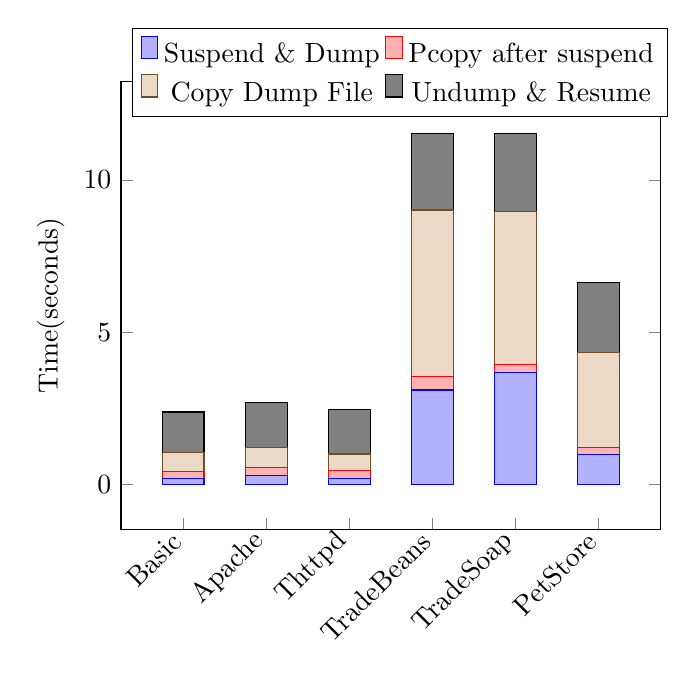
\begin{tikzpicture}
      \begin{axis}[
        ybar stacked,
        bar width=15pt,
        %	nodes near coords,
        enlargelimits=0.15,
        legend style={at={(0.02,1.12)},anchor=north west,legend columns=2},
        ylabel={Time(seconds)},
        symbolic x coords={Basic, Apache, Thttpd, TradeBeans, TradeSoap, 
          PetStore},
        xtick=data,
        x tick label style={rotate=45,anchor=east},
        ]
        \addplot+[ybar] plot coordinates {(Basic,0.21) (Apache,0.30) (Thttpd,0.21) (TradeBeans,3.10) (TradeSoap,3.68) (PetStore,0.97) };
        \addplot+[ybar] plot coordinates {(Basic,0.22) (Apache,0.27) (Thttpd,0.26) (TradeBeans,0.44) (TradeSoap,0.25) (PetStore,0.24) };
        \addplot+[ybar] plot coordinates {(Basic,0.62) (Apache,0.64) (Thttpd,0.53) (TradeBeans,5.47) (TradeSoap,5.03) (PetStore,3.11) };
        \addplot+[ybar] plot coordinates {(Basic,1.33) (Apache,1.47) (Thttpd,1.46) (TradeBeans,2.51) (TradeSoap,2.57) (PetStore,2.32) };
        \addlegendentry{\strut Suspend \& Dump}
        \addlegendentry{\strut Pcopy after suspend}
        \addlegendentry{\strut Copy Dump File}
        \addlegendentry{\strut Undump \& Resume}
      \end{axis}
    \end{tikzpicture}
   }
  %\captionsetup{justification=centering}
  \caption{Suspend time for live cloning, when running a representative benchmark}
  \label{fig:stats}
\end{figure}


\subsubsection{Real world applications and workloads:}
To begin to study the overhead of live cloning, we performed an evaluation using five well-known applications.
Figure~\ref{fig:stats} presents the suspended times for five well-known applications when cloning a replica with \parikshan. 
We ran the httperf~\cite{httperf} benchmark on Apache and \emph{thttpd} to compute max throughput of the web-servers, by sending a large number of concurrent requests.
Tradebeans and Tradesoap are both part of the dacapo~\cite{dacapo} benchmark ``DayTrader'' application.
These are realistic workloads, which run on a multi-tier trading application provided by IBM. 
PetStore~\cite{petstore} is also a well known J2EE reference application. 
We deployed PetStore in a 3-tier system with JBoss, MySQL and Apache servers, and cloned the app-server.
The input workload was a random set of transactions which were repeated for the duration of the cloning process.

As shown in Figure~\ref{fig:stats}, for Apache and Thttpd the container suspend time ranged between 2-3 seconds.
However, in more memory intensive application servers such as PetStore and DayTrader, the total suspend time was higher (6-12 seconds).
Nevertheless, we did not experience any timeouts or errors for the requests in the workload\footnote{In case of packet drops, requests are resent both at the TCP layer, and the application layer. This slows down the requests for the user, but does not drop them}.
However, this did slowdown requests in the workload. 
This shows that short suspend times are largely not visible or have minimal performance impact to the user, as they are within the time out range of most applications.
Further, a clean network migration process ensures that connections are not dropped, and are executed successfully.
We felt that these relatively fast temporary app suspensions were a reasonable price to pay to launch an otherwise overhead-free debug replica.
To further characterize the suspend time imposed by the live cloning phase of \parikshan, we created a synthetic micro-benchmark to push \parikshan towards its limit.
\begin{figure}[ht]
%{0.45\textwidth}
  \centering
  \resizebox{.8\linewidth}{!}{
%\begin{adjustbox}{max size={.9\textwidth}}
    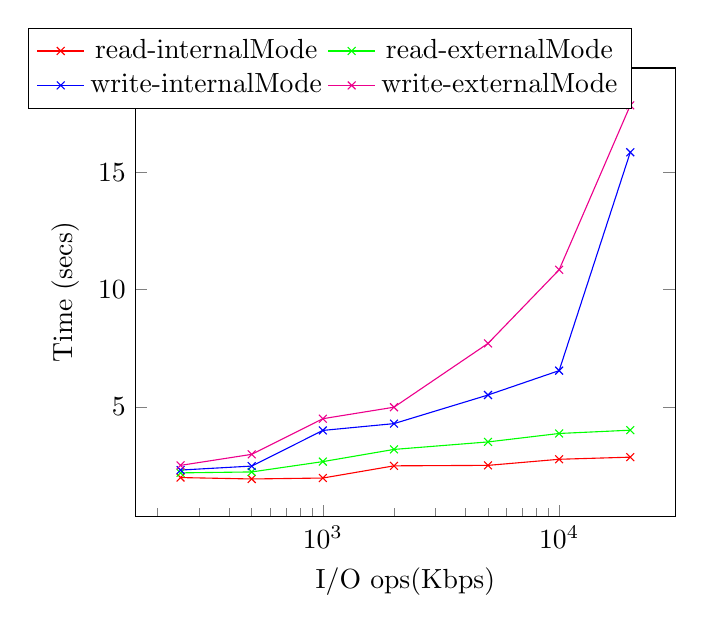
\begin{tikzpicture}
      \begin{axis}[
        xmode=log,
        legend style={at={(-0.2,1.09)},anchor=north west,legend columns=2},
        xlabel=I/O ops(Kbps),
        ylabel=Time (secs)]
        \addplot[color=red,mark=x] coordinates {
          (0,1.85)
          (250,1.99)
          (500,1.93)
          (1000,1.97)
          (2000,2.49)
          (5000,2.51)
          (10000,2.77)
          (20000,2.86)
        };
        \addlegendentry{read-internalMode}
        \addplot[color=green,mark=x] coordinates {
          (0,1.97)
          (250,2.19)
          (500,2.23)
          (1000,2.67)
          (2000,3.19)
          (5000,3.51)
          (10000,3.87)
          (20000,4.01)
        };
        \addlegendentry{read-externalMode}				
        \addplot[color=blue,mark=x] coordinates {
          (0,1.85)
          (250,2.31)
          (500,2.48)
          (1000,4.00)
          (2000,4.29)
          (5000,5.51)
          (10000,6.55)
          (20000,15.86)
        };
        \addlegendentry{write-internalMode}				
        \addplot[color=magenta,mark=x] coordinates {
          (0,1.87)
          (250,2.51)
          (500,2.98)
          (1000,4.50)
          (2000,4.99)
          (5000,7.71)
          (10000,10.85)
          (20000,17.86)
        };
        \addlegendentry{write-externalMode}
      \end{axis}
    \end{tikzpicture}
 % \end{adjustbox}
  }
  %\captionsetup{justification=centering}
  \caption{Live Cloning suspend time with increasing amounts of I/O operations }
  \label{fig:fioResults}
\end{figure}



\subsubsection{Micro Benchmark using I/O operations:}
The main factor that impacts suspend time is the number of ``dirty pages'' in the suspend phase, which have not been copied over in the pre-copy rsync operation (see section~\ref{sec:CloneManager}).
To understand this better, we use \fio (flexible I/O tool for Linux)~\cite{fio}, to gradually increase the number of I/O operations while doing live cloning.
We run the \fio tool to do read and writes of random values with a controlled I/O bandwidth. 
%The suspend time is observed by instrumentation within the cloning script, which reports time taken by each of the suspend processes.
Additionally, we ensure that the I/O job being processed by \fio is long enough to last through the cloning process.

As shown in figure~\ref{fig:fioResults}, read operations have a much smaller impact on suspend time of live cloning compared to write operations.
This can be attributed to the increase of ``dirty pages'' in write operations, whereas for read, the disk image remains largely the same.
The internal mode is much faster than the external mode, as both the production and debug-container are hosted in the same physical device.
We believe, that for higher I/O operations, with a large amount of ``dirty-pages'', network bandwidth becomes a bottleneck: leading to longer suspend times.
Overall in our experiments, the internal mode is able to manage write operation up to 10 Mbps, with a total suspend-time of approx 5 seconds.
Whereas, the external mode is only able to manage up to 5-6 Mbps, for a 5 sec suspend time.\\ \\


\input{parikshan/windowEval}

%\subsection{A survey of real-world bugs}
\label{sec:survey}
\noindent

In Table~\ref{tab:survey}, we present the results of a survey of bug reports of three production SOA applications.
In order to understand how we did the survey, let us look at MySQL as an example.
We first searched for bugs which were tagged as ``fixed'' by developers and dumped them.
We then chose a random time-line (2013-2014) and filtered out all bugs which belonged to non-production components - like documentation, installation failure, compilation failure.
We then manually went through each of the bug-reports, filtering out the ones which were mislabeled or were reported based on code-analysis, or did not have a triggering test report (essentially we focused only on bugs that happened during production scenarios).
We then classified these bugs into the categories shown in Table~\ref{tab:survey} based on the bug-report description, and the patch fix, to-do action item for the bug.

One of the core-insights provided by this survey was that most bugs (93\%) triggered in production systems are deterministic in nature (everything but concurrency bugs), among which the most common ones are semantic bugs (80\%).
This is understandable, as they usually happen because of unexpected scenarios or edge cases, that were not thought of during testing.
Recreation of these bugs depend only on the state of the machine, the running environment (other components connected when this bug was triggered), and network input requests, which trigger the bug scenario.
\parikshan is a useful testing tool for testing these deterministic bugs in an exact clone of the production state, with replicated network input. 
The execution can then be traced at a much higher granularity than what would be allowed in production containers, to find the root cause of the bug. 

On the other hand, concurrency errors, which are non-deterministic in nature make up for less than 7\% of the production bugs.
Owing to non-determinism, it is possible that the same execution is not triggered. However concurrent points can still be monitored and a post-facto search of different executions can be done to find the bug~\cite{dpor,systematicDPORconcurrency} to capture these non-deterministic errors.\\ \\


\begin{table}[]
\centering
\begin{tabular}{cccc}
\toprule
\textbf{Category} & \textbf{Apache} & \textbf{MySQL} & \textbf{HDFS} \\ \midrule
\textbf{Performance} & 3 & 10 & 6 \\ 
\textbf{Semantic} & 36 & 73 & 63 \\ 
\textbf{Concurrency} & 1 & 7 & 6 \\ 
\textbf{Resource Leak} & 5 & 6 & 1 \\ \midrule
\textbf{Total} & 45 & 96 & 76 \\
\bottomrule
\end{tabular}
\caption{Survey and classification of bugs}
\label{tab:survey}
\end{table}




\section{Discussion and Limitations}
\label{sec:parikshanThreats}

Through our case studies and evaluation, we concluded that \parikshan can faithfully reproduce many real bugs in complex applications with no running-overhead.
However, there may be several threats to the validity of our experiments.
For instance, in our case study, the bugs that we selected to study may not be truly representative of a broad range of different faults.
Perhaps, \parikshan's low-overhead network record and replay approach is less suitable to some classes of bugs.
To alleviate this concern, we selected bugs that represented a wide range of categories of bugs, and further, selected bugs that had already been studied in other literature, to alleviate a risk of selection bias.
We further strengthened this studied with a follow-up categorization of 217 bugs in three real-world applications, finding that most of those bugs were semantic in nature, and very few were non-deterministic, and hence, having similar characteristics to those 16 that we reproduced. \\

\noindent There are also some underlying limitations and assumptions regarding \parikshan's applicability:

\xxx{Clarify what exactly we can and cannot do WRT non-determinism and distirbuted services.}


\subsection{Non-determinism} 
\label{sec:parikshanThreatsNonDeterminism}
Non-determinism can be attributed to three main sources (1) system configuration, (2) application input, and (3) ordering in concurrent threads.
Live cloning of the application state ensures that both applications are in the same ``system-state'' and have the same configuration parameters for itself and all dependencies.
%Furthermore, in offline debugging it is often difficult to capture all possible inputs, and hence deal with input non-determinism.
\parikshan's network proxy ensures that all inputs received in the production container are also forwarded to the debug container.
However, any non-determinism from other sources (e.g. thread interleaving, random numbers, reliance on timing) may limit \parikshan's ability to faithfully reproduce an execution. 
%However, concurrency based non-determinism can still lead to different execution paths in the production and debug containers.
While our current prototype version does not handle these, we believe there are several existing techniques that can be applied to tackle this problem in the context of live debugging.
However, as can be seen in our case-studies above, unless there is significant non-determinism, the bugs will still be triggered in the replica, and can hence be debugged. 
Approaches like statistical debugging~\cite{Liblit:2004:CBI}, can be applied to localize bug.
%Furthermore, techniques like deterministic scheduling~\cite{smt:cacm}, can also be used to counter concurrency based bugs.
\parikshan allows debugger to do significant tracing of synchronization points, which is often required as an input for constraint solvers~\cite{dpor,best}, which can go through all synchronization orderings to find concurrency errors.
We have also tried to alleviate this problem using our divergence checker (Section~\ref{sec:parikshanDivergenceChecking})


\subsection{Distributed Services} 
\label{sec:parikshanThreatsDirstributed}

Large-scale distributed systems are often comprised of several interacting services such as storage, NTP, backup services, controllers and resource managers.
\parikshan can be used on one or more containers and can be used to clone more than one communicating .
Based on the nature of the service, it may be (a). Cloned, (b). Turned off or (c). Allowed without any modification.
For example, storage services supporting a replica need to be cloned or turned off (depending on debugging environment) as they would propagate changes from the debug container to the production containers.
Similarly, services such as NTP service can be allowed to continue without any cloning as they are broadcast based systems and the debug container cannot impact it in anyway.
Furthermore, instrumentation inserted in the replica, will not necessarily slowdown all services.
For instance, instrumentation in a MySQL query handler will not slowdown file-sharing or NTP services running in the same container.

\subsection{Overhead in Parikshan}
\label{sec:parikshanOverhead}

The key motivation of \parikshan is to remove all potential overheads such that instrumentation in the debug-container does not impact performance of the production application.
We wish to clarify certain aspects which may lead to questions regarding overheads in the mind of the reader:
\begin{itemize}
	\item \textbf{Container virtualization:} Based on recent studies, user-space container virtualization give near native performance~\cite{performanceComparisonlxcVM,performanceEvalContainers}. 
	User-space containers essentially leverage process level isolation and do not have a full just-in-time virtualization stack.
	Since several existing SOA applications are deployed in virtualized cloud environments (including full virtualization), we believe that there is no additional overhead from \parikshan as far as container virtualization is concerned
	
	\item \textbf{Network Forwarding:} 
	Another potential source of overhead is network forwarding due to in-memory copy of the data packets being forwarded to the debug-container. 
	To evaluate (see section~\ref{sec:end2endEval}) the overhead we looked at how network overhead can impact bandwidth and latency in both raw TCP requests (micro-benchmarks), as well as how it impacted a few real-world applications (wikibench, and mysql).
	When compared to SOA applications with proxies, we found that the impact in both throughput and latency was negligible (max 1-2\%).
	We also verified \textbf{that increasing the overhead in the debug container has no impact on the production service}. 
	Given that proxies are used commonly in deployed web/service level applications, we could clearly demonstrate that duplication does not add any discernible overhead to production services. 
	Web proxies like squid~\cite{squid} are commonly used to give an order of magnitude performance improvement, and reducing system load by caching frequently fetched pages and links.
	\parikshan can easily be coupled with such already existing web proxies in the system thereby not adding a new network hop by introducing it's own proxy.
	
	\item \textbf{Live Cloning:}
	The reader may also be concerned with overhead due to live cloning.
	Live cloning involves a small time during which the machine must be suspended, this can impact the latency of requests.
	Firstly, it is important to point out that live cloning is \textbf{a single-time process (or periodic)}, and does not impact the general processing of requests in the SOA application, when we are not trying to sync with the production container.   
	The amortized cost of this momentary suspend process process on a live running production application is generally considered acceptable (consider that live migration is used in production systems all the time).
	
	The current implementation for live cloning shown in this thesis is derived from early work in live migration in container virtualization of openvz container virtualization~\cite{vzctl}. 
	We designed this mostly for the \emph{purposes of demonstrating a viable prototype} where live cloning is possible.
	While live migration is a relatively well researched topic in full virtualized systems, it is relatively new in container virtualization.
	Furthermore, network file system support can tremendously improve cloning time and decrease suspension time.
	Live migration is actively used in production systems of several well-known cloud service providers such as amazon~\cite{ec2}, google compute~\cite{gcompute} etc.
	With further advancement in live migration technologies in the user-space container virtualization, state-of-art migration techniques can be modified for live-cloning and can help in the adoption of \parikshan with much shorter suspend times.
	

\end{itemize}



\section{Summary}
\label{sec:parikshanSummary}

\parikshan is a novel framework that uses redundant cloud resources to debug production SOA applications in real-time.
Compared to existing monitoring solutions, which have focused on reducing instrumentation overhead, our tool is able to avoid any performance slowdown at all, at the same time potentially allow significant monitoring for the debugger.
We have made \parikshan prototype tool available on GitHub for use by other researchers and practitioners.

%For each of the 16 faults studied in our case study, we have also created a docker containers for most of our experiments, and in the rest we have left a detailed README of the install instructions, and the bug trigger mechanism.
%An extended version of the paper is present in CUCS Tech Reports~\cite{parikshanTR,parikshanQueue}, details about the project, and source code is available on github~\cite{github}. 
%Kaiser is funded in part by NSF CCF-1302269 and CCF-1161079.
%comment{
%We would like to acknowledge Qiang Xu, Abhishek Sharma, and Pallavi Joshi for their insight and feedback in designing \parikshan, and in the evaluation of this technology.
%The authors are affiliated with NEC Labs, Princeton, Google Inc, and Columbia University. 


\chapter{Is network replay enough?}
\label{ch:NetworkReplaySurvey}

\section{Overview}
\label{sec:netReplayOverview}

Several existing record and replay have a much higher overhead as they record low level of non-determinism in order to capture and replay the exact state of execution. 
However, most bugs in service oriented application do not require such low level of recording.
We hypothesize that network input with live cloning is enough to trigger most bugs in user-facing services.

To validate this insight, we selected sixteen real-world bugs, applied \parikshan, reproduced them in a production container, and observed whether they were also simultaneously reproduced in the replica.
For each of the sixteen bugs that we triggered in the production environments, \parikshan faithfully reproduced them in the replica. 

We selected our bugs from those examined in previous studies \cite{bugbench,simpleTesting}, focusing on bugs that involved performance, resource-leaks, semantics, concurrency, and configuration. 
We have further categorized these bugs whether they lead to a crash or not, and if they can be deterministically reproduced.
Table \ref{tab:casestudy} presents an overview of our study.

In the rest of this section we discuss the bug-reproduction technique in each of these case-studies in further detail.

\input{parikshan/casestudy-table1}

\section{Applications Targeted}

In our case-studies we have targeted the following applications: MySQL, Apache, Redis, Cassandra, HDFS. Apart from this we have also tried \parikshan on PetStore~\cite{petstore} a J2EE JBOSS~\cite{jboss} multi-tier application. We also did a survey of 217 real-world bugs, and found them similar to the bugs presented in this case study( more details regarding the survey can be found at section~\ref{sec:parikshanSurvey}).
In this section we explain the applications that have been used in the bug case-studies.

\subsection{MySQL}

MySQL~\cite{mysql} is a well known open-source database application for structured SQL queries. 
MySQL is most commonly deployed as a standalone centralized server, and can also be deployed as a cluster service with several servers sharing the data. 
It allows for atomic updates with strict consistency models, so there is a single point of query, and is usually queried using customized \texttt{MYSQL protocol}, which is avialable in several mysql libraries or clients in different languages.
Several modern websites and transaction systems are built on MySQL.
Other softwares which are very similar in deployment to MySQL are Oracle DB~\cite{oracle}, and PostgrepSQL~\cite{postgresql}.

In our examples we have used the native mysql client application provided with the mysql community server distribution.
When using mysql, you can either use an anonymous user, a registered user or an admin.
We have used the default mysql/mysql user or anonymous user to run our queries.

\subsection{Apache}

Apache httpd server~\cite{apache} is the most well known webservers with millions of active websites being hosted on it.
It responds to \texttt{HTTTP} requests from user-facing browsers, and sends responses from downstream applications to be rendered back in the browser.
Webservers can run standalone, multi-tier in a load-balanced fashion or can act as proxies for security purposes.

\xxx{proxy can be made for HTTP? just add as it's possible}

\subsection{Redis}

\subsection{Cassandra}

\subsection{HDFS}

\section{Case Studies}
\label{sec:parikshanCasestudy}

\xxx{How did we select these bugs? Randomly? How did we try to reproduce them?}

\xxx{This part that was here and I commented out makes no sense in this section - maybe worthwhile moving it to somewhere else to explain *why* someone would use parikshan. but here, we are talking about our core assumption, that network replay is sufficient. This section should be about the study we did to show that this insight is grounded.}


\subsection{Semantic Bugs}
The majority of the bugs found in production SOA systems can be categorized as semantic bugs.
These bugs often happen because an edge condition was not checked during the development stage or there was a logical error in the algorithm etc.
Many such errors result in an unexpected output or possibly can crash the system.
We recreated 4 real-world production bugs from Redis~\cite{redis} queuing system, and Cassandra~\cite{cassandra} a NoSQL database.

\xxx{TODO:Nipun - Add some explanation for Redis, and Cassandra}

\subsubsection{Redis \#761}

In this subsection we describe the Redis\#761 semantic bug \\

\noindent \textbf{Cause of the error:}\\


\noindent The Redis\#761 is an integer overflow error. 
This error is triggered, when the client tries to insert and store a very large number. 
This leads to an unmanaged exception, which crashes the production system. 
Integer overflow, is a common error in several applications. 
We classify this as a semantic bug, which could have been fixed with an error checking condition for large integers. \\


\noindent \textbf{Steps for reproduction:}\\

\begin{adjustwidth}{0.5cm}{}
\begin{enumerate}
	\item Start a redis service with log level set to verbose. Setting loglevel to verbose ensures that we can view whatever is going on inside the service. This is our \productioncontainer.
	\item Create a live clone of the service mapped to a parallel \debugcontainer which will be used to visualize debugging
	\item Start cloning the incoming traffic to both the \productioncontainer and the \debugcontainer asynchronously using \parikshan's network duplicator
	\item Send the following request through the redis client: 
	
		\texttt{zinterstore out 9223372036854775807 zset zset2}
		
		This tries to set the variable to the integer in the request, and leads to an integer overflow error. The integer overflow error is simultaneously triggered both in the production and the debug containers.
	
\end{enumerate}
\end{adjustwidth}

\subsubsection{Redis \#487}

In this subsection we describe the Redis\#487 semantic bug \\

\noindent \textbf{Cause of the error:} \\

Redis\#487 resulted in expired keys still being retained in Redis, because of an unchecked edge condition.
While this error does not lead to any exception or any error report in application logs, it gives the user a wrong output.
In the case of such logical errors, the application keeps processing, but the internal state can stay incorrect.
The bug impacts only clients who set keys, and then expire them.\\

\noindent \textbf{Steps for reproduction:} \\

\begin{adjustwidth}{0.5cm}{}
	\begin{enumerate}
			\item Start a redis service with log level set to verbose. Setting loglevel to verbose ensures that we can view whatever is going on inside the service. This is our \productioncontainer.
			\item Create a live clone of the service mapped to a parallel \debugcontainer which will be used to visualize debugging
			\item Start cloning the incoming traffic to both the \productioncontainer and the \debugcontainer asynchronously using \parikshan's network duplicator
			\item flush all keys using \texttt{flushall} command 
			\item set multiple keys using \texttt{set key value} command 
			\item expire a key from one of them using \texttt{expire s 5} command
			\item run the \texttt{keys *} command. This will list keys which should have expired
	\end{enumerate}

\end{adjustwidth}


At the end it can be seen that the expired keys can be listed and accessed in both the production and debug container. This is a persistent error, which does not impact most other aspects of the service. The debug container can be used to look at the transactional logs, and have further instrumentation to understand the root cause of the error.

\subsubsection{Cassandra \#5225}

In this subsection we describe the Cassandra\#5225 semantic bug \\

\noindent \textbf{Cause of the error:} \\

Missing columns when requesting specific columns from a wide row. 
The data is still in the table, just it might not be returned to the user. 
Taking closer look, Cassandra is reading from the wrong column index. 
A problem was found with the index checking algorithm. 
In fact, it was written in reverse.\\

\noindent \textbf{Steps for reproduction:} \\

\begin{adjustwidth}{0.5cm}{}
	\begin{enumerate}
		\item Start a cassandra service in the production container
		\item Use \parikshan's live cloning facility to create a clone of cassandra in the debug-container.
		\item Connect to cassandra using a python client
		\item Insert a large number of columns into cassandra (so that it is a wide row). For our testing we used \texttt{pycassa} python cassandra client. 
		\item Fetch the columns in a portion of ranges
		\item At the end of this test case you can observe that some columns were dropped in the response to the client.
	\end{enumerate}

\end{adjustwidth}

To facilitate re-creating this bug, we have provided dockerized containers, which install the correct version of Cassandra which has this bug as well as it's dependencies. The re-compilation of the version which has the bug is significantly difficult as some of the dependency libraries are no longer available using simply their Apache IVY build files. We also provide a python script for the cassandra client to trigger the bug conditions.

\subsubsection{Cassandra \#1837}

In this subsection we describe the Cassandra\#1837 semantic bug \\

\noindent \textbf{Cause of the error:} \\

The main symptom of this error was that deleted columns become available again after doing a flush.
With some domain knowledge, a developer found the error. 
This happens because of a bug in a the way deleted rows are not interpreted once they leave the memtable in the CFS.getRangeSlice code i.e. the flush does not recognize the delete and the purged data does not contain the delete operation. 
Thus querying for the data shows  content as well.

\noindent \textbf{Steps for reproduction:} \\

\begin{adjustwidth}{0.5cm}{}
	\begin{enumerate}
		\item Start a cassandra service in the production container
		\item Use \parikshan's live cloning facility to create a clone of cassandra in the debug-container.
		\item Using cassandra's command line client, insert columns into cassandra without flushing
		\item delete the inserted column
		\item flush the columns so that the deletion should be committed
		\item query for the columns in the table
		\item observe that the columns have not been deleted and are retained.
	\end{enumerate}
\end{adjustwidth}

Once again we have provide dockerized containers for Cassandra, as well as execution scripts for the client.

\subsection{Performance Bugs}

These bugs do not lead to crashes but cause significant impact to user satisfaction.
A casestudy~\cite{shanluPerf} showed that a large percentage of real-world performance bugs can be attributed to uncoordinated functions, executing functions that can be skipped, and inefficient synchronization among threads (for example locks held for too long etc.).
Typically, such bugs can be caught by function level execution tracing and tracking the time taken in each execution function.
Another key insight provided in~\cite{shanluPerf} was that two-thirds of the bugs manifested themselves when special input conditions were met, or execution was done at scale. 
Hence, it is difficult to capture these bugs with traditional offline white-box testing mechanisms.


\subsubsection{MySQL \#26257}

In this subsection we describe the MySQL\#15811 performance bug \\

\noindent \textbf{Cause of the error:} \\

\noindent \textbf{Steps for reproduction:} \\

\begin{adjustwidth}{0.5cm}{}
	\begin{enumerate}
		\item Start an instance of the MySQL server in the production container
		\item Using \parikshan's live cloning capability create a clone of the \productioncontainer. This is our \debugcontainer
		\item Start network duplicator to duplicate network traffic to both the production and debug containers
		\item connect to the production container using \texttt{mysqlclient}
		
	\end{enumerate}
\end{adjustwidth}	


\subsubsection{MySQL \#49491}

In this subsection we describe the MySQL\#15811 performance bug \\

\noindent \textbf{Cause of the error:} \\

It was reported that the calculation of MD5 and SHA1 hash values using the built-in MySQL functions does not seem to be as efficient, and takes too long.There seem to be two factors that determine the performance of the hash generation:
\begin{itemize}
	\item computation of the actual hash value (binary value)
	\item conversion of the binary value into a string field
\end{itemize}

The run time of the hash computation depends on the length of the input string whereas the overhead of the binary-to-string conversion can be considered as a fixed constant as it will always operate on hash values of 16 (MD5) or 20 (SHA1) bytes length.
The impact of the binary-to-string conversion will become more visible with shorter input strings than with long input strings. For short input strings it seems that more time is spent in the binary-to-string conversion than in the actual hash computation part.\footnote{A patch provided by a developer improved the performance by an order of magnitude. However for the purposes of our discussion, we have limited ourselves to bug-recreation}

\noindent \textbf{Steps for reproduction:} \\

\begin{adjustwidth}{0.5cm}{}
	\begin{enumerate}
		\item Start an instance of the MySQL server in the production container
		\item Using \parikshan's live cloning capability create a clone of the \productioncontainer. This is our \debugcontainer
		\item Start network duplicator to duplicate network traffic to both the production and debug containers
		\item connect to the production container using \texttt{mysqlclient}
		\item Run a select query from the client on the users database:
		
		\texttt{select count(\*) from (select md5(firstname) from users) sub limit 1G}

		
		\item The time observed for this query is reported as a performance bug by the reporter. This can be viewed both in the production container and the debug container
		
	\end{enumerate}
\end{adjustwidth}	



\subsubsection{MySQL \#15811}

In this subsection we describe the MySQL\#15811 performance bug \\

\noindent \textbf{Cause of the error:} \\

For one of the bugs in  MySQL\#15811, it was reported that some of the user requests which were dealing with complex scripts (Chinese, Japanese), were running significantly slower than others.
To evaluate \parikshan, we re-created a two-tier client-server setup with the server (container) running a buggy MySQL server and sent queries to the production container with complex scripts (Chinese).
These queries were asynchronously replicated, in the debug container. To further investigate the bug-diagnosis process, we also turned on execution tracing in the debug container using SystemTap~\cite{systemtap}.
This gives us the added advantage, of being able to profile and identify the functions responsible for the slow-down, without the tracing having any impact on production.\\

\noindent \textbf{Steps for reproduction:} \\

\begin{adjustwidth}{0.5cm}{}
	\begin{enumerate}
		\item Start an instance of the MySQL server in the production container
		\item Using \parikshan's live cloning capability create a clone of the \productioncontainer. This is our \debugcontainer
		\item Start network duplicator to duplicate network traffic to both the production and debug containers
		\item connect to the production container using \texttt{mysqlclient}
		\item Create a table with default charset as latin1:
			\texttt{create table t1(c1 char(10)) engine=myisam default charset=latin1;}
		\item Repeat the following line several times to generate a large dataset
			\texttt{insert into t1 select * from t1;}
		\item Now create a mysqldump of the table
		\item Load this table back again, and observe a significant slow response for large table insert requests. This is magnified several times when using complex scripts
	\end{enumerate}
\end{adjustwidth}	



\subsection{Resource Leaks}
Resource leaks can be either memory leak or un-necessary zombie processes.
Memory leaks are common errors in service-oriented systems, especially in C/C++ based applications which allow low-level memory management by users.
These leaks build up over time and can cause slowdowns because of resource shortage, or crash the system.
Debugging leaks can be done either using systematic debugging tools like Valgrind, which use shadow memory to track all objects, or memory profiling tools like VisualVM, mTrace, or PIN, which track allocations, de-allocations, and heap size.
Although Valgrind is more complete, it has a very high overhead and needs to capture the execution from the beginning to the end (i.e., needs application restart).
On the other hand, profiling tools are much lighter and can be dynamically patched to a running process.

Let us take Redis\#417 for instance, here we had a redis master and slave set up for both production and debug container.
We then triggered the bug by running concurrent requests through the client which can trigger the memory leak.
The memory leak was easily visible in the debug container by turning on debug tracing, which showed a growing memory usage. 


\subsubsection{Redis \#417}

In this subsection we describe the Redis\#417 performance bug \\

\noindent \textbf{Cause of the error:} \\

\noindent \textbf{Steps for reproduction:} \\

\begin{adjustwidth}{0.5cm}{}
	\begin{enumerate}
		\item Start a redis service with log level set to verbose. Setting loglevel to verbose ensures that we can view whatever is going on inside the service. This is our \productioncontainer.
		\item Create a live clone of the service mapped to a parallel \debugcontainer which will be used to visualize debugging
		\item Start cloning the incoming traffic to both the \productioncontainer and the \debugcontainer asynchronously using \parikshan's network duplicator
	\end{enumerate}
\end{adjustwidth}	


\subsubsection{Redis \#614}

In this subsection we describe the Redis\#614 performance bug \\

\noindent \textbf{Cause of the error:} \\

\noindent \textbf{Steps for reproduction:} \\

\begin{adjustwidth}{0.5cm}{}
	\begin{enumerate}
		\item Start a redis service with log level set to verbose. Setting loglevel to verbose ensures that we can view whatever is going on inside the service. This is our \productioncontainer.
		\item Create a live clone of the service mapped to a parallel \debugcontainer which will be used to visualize debugging
		\item Start cloning the incoming traffic to both the \productioncontainer and the \debugcontainer asynchronously using \parikshan's network duplicator
	\end{enumerate}
\end{adjustwidth}



\subsection{Concurrency Bugs}
One of the most subtle bugs in production systems is caused due to concurrency errors.
These bugs are hard to reproduce, as they are non-deterministic, and may or may not happen in a given execution.
Unfortunately, \parikshan cannot guarantee that if a buggy execution is triggered in the production container, an identical execution will trigger the same error in the debug container.
However, given that the debug container is a live-clone of the production container, and that it replicates the state of the production container entirely, we believe that the chances of the bug also being triggered in the debug container are quite high.
Additionally, the debug container is a useful tracing utility to track thread lock and unlock sequences, to get an idea of the concurrency bug.

\subsubsection{Apache \#25520}

In this subsection we describe the Apache\#25520 performance bug \\

\noindent \textbf{Cause of the error:} \\

\noindent \textbf{Steps for reproduction:} \\

\begin{adjustwidth}{0.5cm}{}
	\begin{enumerate}
		\item Start a redis service with log level set to verbose. Setting loglevel to verbose ensures that we can view whatever is going on inside the service. This is our \productioncontainer.
		\item Create a live clone of the service mapped to a parallel \debugcontainer which will be used to visualize debugging
		\item Start cloning the incoming traffic to both the \productioncontainer and the \debugcontainer asynchronously using \parikshan's network duplicator
	\end{enumerate}
\end{adjustwidth}


\subsubsection{Apache \#21287}

In this subsection we describe the Apache\#21287 performance bug \\

\noindent \textbf{Cause of the error:} \\

\noindent \textbf{Steps for reproduction:} \\

\begin{adjustwidth}{0.5cm}{}
	\begin{enumerate}
		\item Start a redis service with log level set to verbose. Setting loglevel to verbose ensures that we can view whatever is going on inside the service. This is our \productioncontainer.
		\item Create a live clone of the service mapped to a parallel \debugcontainer which will be used to visualize debugging
		\item Start cloning the incoming traffic to both the \productioncontainer and the \debugcontainer asynchronously using \parikshan's network duplicator
	\end{enumerate}
\end{adjustwidth}


\subsubsection{MySQL \#644}

In this subsection we describe the MySQL\#644 performance bug \\

\noindent \textbf{Cause of the error:} \\

\noindent \textbf{Steps for reproduction:} \\

\begin{adjustwidth}{0.5cm}{}
	\begin{enumerate}
		\item Start an instance of the MySQL server in the production container
		\item Using \parikshan's live cloning capability create a clone of the \productioncontainer. This is our \debugcontainer
		\item Start network duplicator to duplicate network traffic to both the production and debug containers
		\item connect to the production container using \texttt{mysqlclient}
	\end{enumerate}
\end{adjustwidth}	


\subsubsection{MySQL \#169}

In this subsection we describe the MySQL\#169 performance bug \\

\noindent \textbf{Cause of the error:} \\

\noindent \textbf{Steps for reproduction:} \\

\begin{adjustwidth}{0.5cm}{}
	\begin{enumerate}
		\item Start an instance of the MySQL server in the production container
		\item Using \parikshan's live cloning capability create a clone of the \productioncontainer. This is our \debugcontainer
		\item Start network duplicator to duplicate network traffic to both the production and debug containers
		\item connect to the production container using \texttt{mysqlclient}
	\end{enumerate}
\end{adjustwidth}	


\subsubsection{MySQL \#791}

In this subsection we describe the MySQL\#791 performance bug \\

\noindent \textbf{Cause of the error:} \\

\noindent \textbf{Steps for reproduction:} \\

\begin{adjustwidth}{0.5cm}{}
	\begin{enumerate}
		\item Start an instance of the MySQL server in the production container
		\item Using \parikshan's live cloning capability create a clone of the \productioncontainer. This is our \debugcontainer
		\item Start network duplicator to duplicate network traffic to both the production and debug containers
		\item connect to the production container using \texttt{mysqlclient}
	\end{enumerate}
\end{adjustwidth}	


\subsection{Configuration Bugs}
Configuration errors are usually caused by wrongly configured parameters, i.e., they are not bugs in the application, but bugs in the input (configuration).
These bugs usually get triggered at scale or for certain edge cases, making them extremely difficult to catch.

A simple example of such a bug is Redis\#957, here the slave is unable to sync with the master.
The connection with the slave times out and it's unable to sync because of the large data.
While the bug is partially a semantic bug, as it could potentially have checks and balances in the code. 
The root cause itself is a lower output buffer limit.
Once again, it can be easily observed in our debug-containers that the slave is not synced, and can be investigated further by the debugger.

\subsubsection{Redis \#957}

In this subsection we describe the Redis\#957 performance bug \\

\noindent \textbf{Cause of the error:} \\

\noindent \textbf{Steps for reproduction:} \\

\begin{adjustwidth}{0.5cm}{}
	\begin{enumerate}
		\item Start a redis service with log level set to verbose. Setting loglevel to verbose ensures that we can view whatever is going on inside the service. This is our \productioncontainer.
		\item Create a live clone of the service mapped to a parallel \debugcontainer which will be used to visualize debugging
		\item Start cloning the incoming traffic to both the \productioncontainer and the \debugcontainer asynchronously using \parikshan's network duplicator
	\end{enumerate}
\end{adjustwidth}


\subsubsection{HDFS \#1904}

In this subsection we describe the HDFS\#1904 performance bug \\

\noindent \textbf{Cause of the error:} \\

\noindent \textbf{Steps for reproduction:} \\

\begin{adjustwidth}{0.5cm}{}
	\begin{enumerate}
		\item Start a redis service with log level set to verbose. Setting loglevel to verbose ensures that we can view whatever is going on inside the service. This is our \productioncontainer.
		\item Create a live clone of the service mapped to a parallel \debugcontainer which will be used to visualize debugging
		\item Start cloning the incoming traffic to both the \productioncontainer and the \debugcontainer asynchronously using \parikshan's network duplicator
	\end{enumerate}
\end{adjustwidth}

\section{Summary}
\label{sec:parikshanCaseStudySummary}




\part{\iprobe: An intelligent compiler assisted dynamic instrumentation tool}
\chapter{iProbe}
\label{ch:iprobe}

\section{Introduction}
\label{sec:iProbeIntro}

As explained in section~\ref{sec:intro}, our initial investigation towards low-overhead on-the-fly debugging involved investigating instrumentation strategies which would allow us to dynamically instrument the application, with the least possible overhead.
Intuitively the least possible overhead of any instrumentation in an application is possible when it was already a part of the source-code, and not added as an after-thought when required for instrumentation.
However, source-code level instrumentation is "always on" and has an overhead all the time on the application.
Hence, our goal was to have a production system tracing tool should have zero-overhead when it is not activated and should have the least possible overhead when it is activated (we believe source code level instrumentation would have the least overhead as it would not have any overhead inserted by the tool itself). 
At the same time, it should be flexible enough so as to meet versatile instrumentation needs at run-time for management tasks such as trouble-shooting or performance analysis.

Over the years researchers have proposed many tools to assist in application performance analytics \cite{pin,gdb,dtrace,systemtap,lttng,utrace,ptrace,dyninst}.
While these techniques provide flexibility, and deep granularity in instrumenting applications, they often trade in considerable complexity in system design, implementation and overhead to profile the application. 
For example, binary instrumentation tools like Intel's PIN Instrumentation tool \cite{pin}, DynInst \cite{dyninst} and GNU debugger \cite{gdb} allow complete blackbox analysis and instrumentation but incur a heavy overhead, which is unacceptable in production systems. 
Inherently, these tools have been developed for the development environment, hence are not meant for a production system tracer.
Production system tracers such as DTrace\cite{dtrace} and SystemTap\cite{systemtap} allow for low overhead kernel function tracing.
These tools are optimized for inserting hooks in kernel function/system calls, and can monitor run-time application behavior over long time periods. 
However, they have limited instrumentation capabilities for user-space instrumentation, and incur a high overhead due to frequent kernel context-switches and complex trampoline mechanisms.

Software developers often utilize program print statements, write their own loggers, or use tools like log4j~\cite{log4j} or log4c~\cite{log4c} to track the execution of their applications.
Those manually instrumented probe points can easily be deployed without additional libraries or kernel support, and have a low overhead to run without impacting the application performance noticeably. 
However, they are inflexible and can only be turned on/off at compile-time or before starting the execution. 
Besides, usually only a small subset of functions is chosen to avoid larger overheads.

In this chapter, we introduce a dynamic instrumentation framework called \emph{iProbe}.
iProbe has instrumentation overheads comparable to print/debug statements, while still giving users the flexibility to choose targets in the execution stage. 
We evaluated iProbe on micro-benchmark and SPEC CPU 2006 benchmarks.
iProbe showed an order of magnitude performance improvement in comparison to SystemTap\cite{utrace} and DynInst\cite{dyninst} in terms of tracing overhead and scalability.
Additionally, the instrumented applications incur negligible overhead when iProbe is not activated.
We also present a new hardware event profiling tool called \emph{FPerf} developed in the iProbe framework.  
FPerf leverages iProbe's flexibility and scalability to realize a fine-grained performance event profiling solution with overhead control.
In the evaluation, FPerf was able to obtain function-level hardware event breakdown on SPEC CPU2006 applications while controlling performance overhead (e.g., under 5\%)

%so that application usage has a minimal effect is not effected while allowing for application monitoring.
%Another category is tools such as log4j, and log4c \cite{log4j,log4c} that are dependent on user inserted calls to logging functionality.
%Developers can use these tools to add switches for different verbosity levels in application logs, and also these logs can be turned on/off at the beginning of execution or at compile time. 
%While such logging tools have low overhead as they insert instrumentation at compile time (thereby avoiding complexities present in dynamic instrumentation mechanisms), they offer low to no flexibility as logging points are predefined and segregated in levels.

%\subsection{Contributions}

%Over the years researchers have proposed several tools to assist in application performance analytics \cite{pin,gdb,dtrace,systemtap,lttng,utrace,ptrace}. 
%These techniques trade in considerable complexity in system design, implementation and in some cases overhead to gather performance analysis data. 
%For example, binary instrumentation tools like Intel's PIN Instrumentation tool \cite{pin} and GNU debugger \cite{gdb} allow complete blackbox analysis and instrumentation but incur a heavy overhead, which is unacceptable in production systems.  
%Kernel monitoring tools such as Solaris's DTrace \cite{dtrace}, and SystemTap \cite{systemtap} offer a lighter user-space probes to capture the execution of program functions, but still have a comparatively heavy overhead and cannot scale well as they involve software interrupts and context-switches to the kernel to capture the target instructions

% Nipun-> Dtrace, Systemtap are commonly used so should this be put in: \footnote{Most of these tools are primarily kernel space debuggers and work well for kernel function tracing}.  

%On the other hand code-level solutions such as log4j \cite{log4j} are extremely light weight, as they are a part of the target program itself. 
%However, they rely on the programmer modifying the source code ahead of time, and cannot be dynamically changed at run-time to take care of an unseen scenario. 

%challenges with existing dynamic instrumentation tools
%1. high kernel trapping overhead 
%2. can't handle commerical software release with stripped metadata

%iProbe is a user-space monitoring tool 
%that can be packaged with the target application, and 
%that provides a significantly light-weight, flexible, and scalable run-time instrumentation framework. 
The main idea in iProbe design is \emph{decoupling the process of run-time instrumentation into offline and and online stages}, which avoids several complexities faced by current state-of-the-art mechanisms \cite{dtrace,systemtap,dyninst,pin} such as instruction overwriting, complex trampoline mechanisms, and code segment memory allocation, kernel context switches etc.
Most existing dynamic instrumentation mechanisms rely on a trampoline based design, and generally have to make several jumps to get to the instrumentation function as they not only do instrumentation but also simulate the instructions that have been overwritten.
Additionally, they have frequent context-switches as they use kernel traps to capture instrumentation points, and execute the instrumentation.
The performance penalty imposed by these designs are unacceptable in a production environment.


Our design avoids any transitions to the kernel which generally causes higher overheads, and is completely in user space. 
iProbe can be imagined as a framework which provides a seamless transition from an instrumented binary to a non-instrumented binary.
We use a hybrid 2-step mechanism which offloads dynamic instrumentation complexities to an offline development stage, thereby giving us a much better performance.
The following are the 2 stages of iProbe:
\begin{itemize}

\item \textbf{ColdPatch:} We first prepare the target executable by introducing dummy instructions as ``place-holders'' for hooks during the development stage of the application. 
This can be done in 3 different ways: Primarily, we can leverage compiler based instrumentation to introduce our ``place-holders''. 
Secondly we can allow users to insert macros for calls to instrumentation functions which can be turned on and off at run-time. 
Lastly we can use static binary rewriter to insert place-holders in the binary without any recompilation.  
iProbe uses binary parsers to capture all place-holders in the development stage and generates a meta-data file with all possible probe points created in the binary.

\item \textbf{HotPatch:} We then leverage these place-holders during the execution of the process to safely replace them with calls to our instrumentation functions during run-time. 
iProbe uses existing tools, ptrace \cite{ptrace}, to modify the code segment of a running process, and does safety check to ensure correctness of the executing process. 
Using this approach in a systematic manner we reduce the overhead of iProbe while at the same time maintaining a relatively simple design. 


\end{itemize}

We propose a new paradigm in development and packaging of applications, wherein developers can insert probe points in an application by using compiler flag options, and applying our ColdPatch.
An iProbe-ready application can then be packaged along with the meta-data information and deployed in the production environment.
iProbe has negligible effect on the application's performance when instrumentation is not activated, and low overhead when instrumentation is activated. 
We believe this is an useful feature as it requires minimal developer effort, and allows for low overhead production-stage tracing which can be switched on and off as required. 
This is desirable in long-running services for both debugging and profiling usages. 

\iprobe can be used \textbf{individually as a stand-alone tool for instrumentation purposes}, which can assist debuggers in capturing execution traces from production service oriented applications.
Alternatively, it can also be used to \textbf{complement \parikshan in the \debugcontainer} to help us debug applications as a useful instrumentation utility.
MySQL bug\#15811 presented in section~\ref{sec:mySQL15811} is an example of a bug, debugged using \iprobe in \parikshan's \debugcontainer.

%Our tool is system agnostic and works on native applications. 
%We have tested it on large scale systems like mysql and apache, and have evaluated it's performance on the SPEC CPU benchmarks.

%Instead of traditional development approaches which require considerable user effort to add logging points in an application

%iProbe utilizes a novel compiler assited hot-patching technique.  
%Hot Patching has long been studied for security exploits or patching security updates, bug-fixes etc. \cite{katana}. 
%HotPatching is a run-time instrumentation technique which can modify loaded code segments. Previously hot-patching approaches have been used 
%approaches such as windows hot-patching \cite{whotpatch}, live-patch
%and pannus \cite{pannus}, have been used to hot-patch updates, in
%production systems. However, they cannot be used for monitoring as
%they replace the target module entirely and need knowledge of the
%functionality of the target.  

%iProbe revisits old hot-patching mechanisms, to precisely patch instrumentation when required in each functions of the binary. 
%We do this by using compiler driven techniques to introduces placeholders, which assist us as pointers in run-time to do hot-patching. 
%iProbe uses binary parsers to capture all placeholders before the instrumentation and use existing technologies such as ptrace \cite{ptrace} to introduce the patches. 


%iProbe has an order of magnitude less overhead and scales significantly better compared to existing tracing mechanisms such as SystemTap \cite{systemtap}. Further iProbe does not rely on symbolic information in the binary to introduce instrumentation unlike pure black-box binary tracing techniques. This allows for iProbe to trace production binaries with no debug/symbolic information and allows for a smaller light-weight executable, as well as introduces a measure of security from reverse engineering mechanisms.



%\noindent \textbf{Key Features}:
%The following are the key features of iProbe.

%\begin{itemize}

%\item \textbf{Low runtime overhead due to complete user-space design}
%
%State-of-the-art tools such as DTrace \cite{dtrace}, SystemTap \cite{systemtap} and dyninst\cite{dyninst} are sub-optimal in terms of performance, and can generally not scale well.
%fast compared to more fine level monitoring tools such as debuggers \cite{gdb} or dynamic translation tools \cite{pin}.
%However, they still have substantial overhead and cannot be used for persistent monitoring of application level functions in the user-space.
%iProbe introduces a low overhead monitoring which is an order of magnitude faster and scales significantly better than existing mechanisms.


%\item \textbf{Near zero efforts to support run-time instrumentation of applications (hot-patching)}
%\item \textbf{Reliable dynamic instrumentation with near zero runtime efforts}
%

%The dynamic instrumentation requires to patch program status at run-time. 
%Conventional approaches based on trampolines impose the issues on the complexity and reliability of instrumented code such as creating and managing code memory regions for the new control flow \cite{katana,dtrace,systemtap}.
%iProbe create hooks' place holders in the static binary patching then performs runtime instrumentation which enables or disables instrumentation in a more elegant and reliable way by using in-place holders.
%which avoids these complexities. 

%\item \textbf{Support stripped binaries without any debugging information}
%Current approaches such as SystemTap\cite{systemtap}, DTrace\cite{dtrace} require debugging information in the binary for instrumentation.
%iProbe can dynamically instrument binaries at runtime without any debug related information in the deployment by converting the required information to the meta data which is securely managed and used only by iProbe. 
%This design separating the deployment of software and its tracing capability improves the usability of software tracing in the deployment stage, by making the binary light weight and more secure.

%\end{itemize}

The rest of the chapter is organized as following. 
Section \ref{sec:iprobeDesign} discusses the design of iProbe framework, explaining our ColdPatching, and HotPatching techniques;
we also discuss how safety checks are enforced by iProbe to ensure correctness, and some extended options in iProbe for further flexibility.
Section \ref{sec:trampoline} compares traditional trampoline based approaches with our hybrid approach and discusses why we perform, and scale better.
Section \ref{sec:Implementation} explains the implementation of iProbe, 
and describes \emph{FPerf} a tool developed using iProbe framework. 
In section \ref{sec:eval} we evaluate the iProbe prototype, 
and section \ref{sec:iProbeSummary} summarizes this chapter.


\section{Design}
\label{sec:design}

In this section we present the design of iProbe.
Additionally, we then explain some safety checks imposed by iProbe that ensure the correctness of our instrumentation scheme. 
Finally, we discuss extended iProbe modes, static binary rewriting and user written macros, which serve as alternatives to the default compiler-based scheme to insert instrumentation in the pre-processing stage of iProbe.

\begin{figure}[t]
  \begin{center}
    \includegraphics[width=0.75\textwidth]{iprobe/Images/coldpatch.eps}
    \caption{The Process of ColdPatching.}
    \label{fig:coldpatch}
  \end{center}
\end{figure}

The first phase of our instrumentation is an offline pre-processing stage to make the binaries ready for runtime instrumentation. We call this phase \emph{ColdPatching}. 
%meaning the static offline binary patch which is the opposite term to HotPatching to be explained next. 
The second phase is the an online \emph{HotPatching} stage which instruments the monitored program dynamically at runtime without shutting down and restarting the program. 
Next, we present the details of each phase.

%The current implementation of iProbe has been applied and tested in x86 32 bit and 64 bit systems on an centos 5.0, ubuntu, and red-hat system. Technically, however the implementation can be applied to any existing system by using compiler assistance and HotPatching.

\subsection{ColdPatching Phase}
\label{sec:coldpatch}


ColdPatching is a pre-processing phase which generates the place-holders for hooks to be replaced with the calls for instrumentation. 
This operation is performed offline before any execution by statically patching the binary file. 
This phase is composed of three internal steps that are demonstrated in Figure \ref{fig:coldpatch}. 

\begin{itemize}

\item Firstly, iProbe uses compiler techniques to insert instrumentation calls at the beginning and end of each function call. 
The instrumentation parameters, are decided on the basis of the design of the compiler pass. 
The current implementation by default passes callsite information and the base stack pointer as they can be used to inspect and form execution traces. 
Calls to the these instrumentation functions must be \emph{cdecl} calls so that stack correctness can be maintained, this is discussed in further detail in Section \ref{sec:safety}.

\item Secondly, iProbe parses the executable and replaces all instrumentation calls with a \texttt{NOP} instruction which is a no-operation or null instruction. 
This generates instructions in the binary which does no-operation, hence has a negligible overhead, and acts as an empty space for iProbe to be overwritten at run-time.

\item Thirdly, iProbe parses the binary and gathers meta-data regarding all the target instrumentation points into a \emph{probe-list}.
Optionally, iProbe can strip away all debug and symbolic information in the binary making it more secure and light-weight. 
The probe-list is securely transferred to the run-time interface of iProbe and used to probe the instrumentation points. 
Hence iProbe does not have to rely on debug information at run-time to HotPatch the binaries.

%In this way, iProbe differs from existing mechanisms as it does not rely on availability of debug information at run-time to HotPatch the binaries. 
\end{itemize}

%To allow for safe instrumentation using iProbe we need to prepare the target application binary. As described in section.\ref{sec:hotpatch}, to enable HotPatching there must be space allocated in the code segment of the binary to re-write instruction.Existing methodologies overwrite target instructions (eg. the starting instruction of the target instruction with a jump). However, this requires several additional steps to allocate memory and ensure sanity of the stack frames. 

%\indent To reduce complex binary transformations, we prepare the binary for run-time instrumentation before execution by using a coldpatch process.The steps of this process are shown in the state diagram shown in figure \ref{fig:state_rep}. 

%*** Longer version

%The first state is an instruction dump of an unmodified normal binary. As can be seen the initial instructions in each function after the call is made to the function are setting up the stack frame and then the main body. Hence, if any of these instructions are overwritten that would lead to potentially illegal execution states. Instead iProbe makes these binaries \textit{``HotPatch ready``} by introduce place holders in the binary which are used to create empty space. While a compiler transform or flag can be designed based on the target abstraction for instrumentation, for the sake of simplicity we use existing compiler flag options such as ``-finstrument-functions" \cite{gcc_codegen}. As shown in the figure.\ref{fig:state_rep} this flag option generates instrumentation calls at the entry and exit of every function. Just after the entry and before the exit of every function, calls are placed to \emph{\_cyg\_profile\_func\_enter} and \emph{\_cyg\_profile\_func\_exit}. 

%As step 2, we use a binary parser performs a linear scan to search and replace each of these function calls with a NOP instruction (state 3). The replacement needs to be done carefully to ensure that there is enough space to overwrite these NOP's with a call to our instrumentation function. Additionally we store the instruction pointer of each of these function calls, the function they belong to, and the symbolic name. By replacing each of these function calls with NOP instructions we introduce a ``zero-probe" effect in the binary, i.e. the modified binary executes the same as the original binary with negligible overhead.

%To counter address space layout randomization, we also capture offsets with the starting address of each binary. These offsets allow us to use the starting/load address as a anchor to do the instrumentation. In practice we found that the offsets compared to the load address of the executable in binary remain the same, even if load points may be changed.

%One of the advantages of preparing and using the ColdPatching approach is that natural abstractions in the build process can also be used to choose the scope of instrumentation. Instrumentation scope defines the libraries, files, functions, and modules that can be instrumented. iProbe can be used to pre-define the target files, libraries etc. to be compiled, this can be important in cases where the source code is only partially available to the user. This is common for many large scale projects which use proprietary 3rd party components.


\begin{figure*}[t]
  \begin{center}
    \includegraphics[width=0.99\textwidth]{iprobe/Images/state-diagram.eps}
    \caption{Native Binary, the State Transition of ColdPatching and
    HotPatching.}
    \label{fig:state_rep}
  \end{center}
\end{figure*}

\begin{figure}[t]
  \begin{center}
    \includegraphics[width=0.75\textwidth]{iprobe/Images/HotTracing.eps}
    \caption{HotPatching Workflow.}
    \label{fig:hottracing}
  \end{center}
\end{figure}

\subsection{HotPatching Phase}
\label{sec:hottracing}

Once the application binary has been statically patched (i.e., ColdPatched), instrumentation can be applied at runtime. 
Compared to existing trampoline approaches, \emph{iProbe does not overwrite any instructions in the original program, or allocate additional memory} when patching the binaries, and still ensures reliability. 
In order to have a \emph{low overhead}, and \emph{minimal intrusion} of the binary, iProbe avoids most of the complexities involved in HotPatching such as allocation of extra memory in the code segment or scanning code segments to find instrumentation targets in an offline stage. 
The process of HotPatching is as follows: \\
%
%The iProbe run-time hot-tracer is a separate process which monitors the target application. 

\begin{itemize}

\item Firstly, iProbe loads the relevant instrumentation functions in a shared library to the code-segment of the target process. 
This along with allocation of \texttt{NOP}s in the ColdPatching phase allows iProbe to avoid allocation of memory for instrumentation in the code segment. 

\item The probe-list generated in the ColdPatching phase is given to our run-time environment as a list of target probe points in the executable. 
iProbe can handle stripped binaries due to previous knowledge of the target instructions in the ColdPatching.

\item As shown in Figure \ref{fig:hottracing}, in our instrumentation stage, 
our HotPatcher attaches itself to the target process and issues an interrupt (time T1). 
It then performs a reliability check (see Section \ref{sec:safety}), 
and subsequently replaces the \texttt{NOP} instructions in each of the target functions, with a call to our instrumentation function. 
This is a key step which enables iProbe to avoid the complexity of traditional trampoline \cite{livepatch,katana} by not overwriting any logical instructions (non-\texttt{NOP}) in the original code. 
Since the place-holders (\texttt{NOP} instructions) are already available, iProbe can seamlessly patch these applications without changing the size or the runtime footprint of the process. 
Once the calls have been added iProbe releases the interrupt and let normal execution proceed (time T2).

\item At the un-instrumentation stage the same process is repeated, with the exception that the target functions are again replaced with a \texttt{NOP} instruction. 
The period between time T2 and time T3 is our monitoring period, wherein all events are logged to a user-space shared memory logger.

\end{itemize}

\noindent \textbf{State Transition Flow}: \quad Figure \ref{fig:state_rep} demonstrates the operational flow of iProbe in the example to instrument the entry and exit of the \texttt{func\_foo} function. 
The left most figure represents the instructions of a native binary. 
As an example, it shows three instructions (i.e., push, pop, inc) in the prolog and one instruction (i.e., pop) in the epilog of the function \texttt{func\_foo}. 
The next figure shows the layout of this binary when it is compiled with the instrumentation option. 
As shown in the figure, two function calls, \texttt{foo\_begin} and \texttt{foo\_end} are automatically inserted by the compiler at the start and end of the function respectively. 
iProbe exploits these two newly introduced instructions as the place-holders for HotPatching. 
The ColdPatching process overwrites two call instructions with \texttt{NOP}s. 
At runtime, the instrumentation of \texttt{func\_foo} is initiated by HotPatching those instructions with the call instructions to the instrumentation functions: \texttt{begin\_instrument} and \texttt{end\_instrument}. 
This is illustrated in the right most figure in Figure \ref{fig:state_rep}.

\noindent \textbf{Logging Functions and Monitoring Dispatchers} : \quad
%
The calls from the target function to the instrumentation function are generally defined in the coldpatch stage by the compiler. 
However, iProbe also provides monitoring dispatchers which are common instrumentation functions that are shared by target functions. 
Our default instrumentation passes the call site information, and the function address of the target function as parameters to the dispatchers. 
Each monitoring event can be differentiated by these dispatchers using a quick hashing mechanism representing the source of each dispatch.
This allows iProbe to uniquely define instrumentation for each function at run-time, and identify its call sites.

\subsection{Safety Checks for iProbe}
\label{sec:safety}

Safety and reliability of the instrumentation technique is a big concern for most run-time instrumentation techniques.
One of the key advantages of iProbe is that because of its hybrid design reliability and correctness issues are handled in a better way inherently.
In this section we discuss how our HotPatch can achieve such properties in details.
%As explained earlier iProbe operates in 3 different modes,(1) compiler-assisted (2) User-macro based, and (3) static binary rewriting.

\indent \textbf{HotPatch check against Illegal instructions}: \quad
Unlike previous techniques iProbe relies on compiler correctness to ensure safety and reliability in its binary mode.
%The resulting instrumented binary in ColdPatch is not only safe but optimized.
To ensure correctness in our ColdPatching phase, we convert call instructions to instrumentation functions with \texttt{NOP} instruction. 
This does not in any way effect the correctness of the binary, except that instrumentation calls are not made. 
To ensure run-time correctness, iProbe uses a safety check when it interrupts the application while HotPatching. 
Our safety check pass ensures that the program counters of all threads belonging to the target applications do not point to the region of code that is being overwritten (i.e. \texttt{NOP} instructions are not overwritten while they are being executed.
This check is similar to those from traditional Ptrace\cite{ptrace} driven debuggers etc \cite{kaho,livepatch,pannus}. 
Here we use the Ptrace \texttt{GETREGS()} call to inspect the program counter, and if it is currently pointing to the target \texttt{NOP} instructions, we allow the execution to move forward before applying the HotPatch. 
Unlike existing trampoline oriented mechanisms iProbe has a small \texttt{NOP} code segments equal to the length of a single call instruction that it overwrites with instrumentation calls, this means that the check can be performed in a fast and efficient manner. 
It is also important to have this check for all threads which share the code-segment, hence the checking must be able to access the process memory map information, and interrupt all the relevant threads.

\indent \textbf{Safe parameter passing to maintain stack consistency}: \quad
An important aspect for instrumentation is the information passed along to the instrumentation function via the parameter values. 
Since the instrumentation calls are defined by the compiler driven instrumentation, the mechanism in which the parameters passed are decided based on the calling convention used by the compiler. \\
Calling conventions can be broadly classified in two types: caller clean-up based, and callee clean-up based. 
In the former the caller is responsible to pop the parameters passed to function, and hence all parameter related stack operations are performed before and after the call instruction inside the code segment of the caller.
In the later however, the callee is responsible to pop the parameters passed to it.
Since parameters are generally passed using the stack it is important to remove them properly to mantain stack consistency. 

To ensure this iProbe enforces that all calls that are made by the static compiler instrumentation must be \emph{cdecl}~\cite{cdecl} calls where the caller performs the cleanup as compared to \emph{std} calls, where the callee performs it. 
%\emph{cdecl} calls push instrumentation parameters before the call, and stack cleanup is also performed by caller function. 
%On the other hand in \emph{std} call convention the stack cleanup is performed by the callee. 
%For simplicity sake, iProbe uses only \emph{cdecl} calls and allows the push and pop operations performed by the caller. 
As the stack cleanup is automatically performed, it maintains stack consistency, and there is a negligible impact in performance due to the redundant stack operations. 
Alternatively for \emph{std} call convention, push instructions could also be converted to \texttt{NOP}s and HotPatched at run-time, we do not do so as a design choice. 

\indent \textbf{Address Space Layout Randomization}: \quad
Another issue that iProbe addresses is ASLR (address space layout randomization), a security measure used in most environments which randomizes the loading address of executables and shared libraries. 
However, since iProbe assumes the full access to the target system, the load addresses are easily available. 
HotPatcher uses the process id of the target to find all load addresses of each binary/shared library and uses them as base offsets to generate correct instruction pointer addresses. 


%\textbf{Developer Driven Macros}
% The developer driven Macros

%\textbf{Static Binary Rewriter}


\subsection{Extended iProbe Mode}
\label{sec:advanced}

%Since the default mode of iProbe is compiler driven using instrumentation flags.
As iProbe ColdPatching requires compiler assistance, it is unable to operate on pre-packaged binary applications.
Additionally, compiler flags generally have limited instrumentation flexibility as they generally operate on a programming language abstraction(eg. function calls, loops etc.).
To provide further flexibility, iProbe provides a couple of extended options for ColdPatching of the application

\subsubsection{Static Binary Rewriting Mode} 
 In this mode we use a static binary rewriter to insert instrumentation in a pre-packaged binary. 
Once all functions are instrumented, we use a ColdPatching script to capture all call sites to the instrumentation functions and convert them to \texttt{NOP} instruction.
While this mode allows us to directly operate on binaries, a downside is that our current static binary instrumentation technique also uses mini-trampoline mechanisms. 
As explained in Section \ref{sec:trampoline} static binary rewriters use trampoline based mechanisms which induces minimum two jumps.
In the ColdPatch phase, we convert calls to the instrumentation function to \texttt{NOP}s, however the jmp operations to the trampoline function, and simulation of the overwritten instructions still remain.
The downside of this approach has a small overhead even when instrumentation is turned off.
However, in comparison to pure dynamic instrumentation approach it reduces the time spent in HotPatching.
This is especially important if the number of instrumentation targets is high, and the target binary is large, as it will increase the time taken in analyzing the binaries. 
Additionally, if compiler options cannot be changed for certain sections of the program (plugins/3rd party binaries), iProbe can still be applied using this extended feature.

Our current implementation uses the dyninst \cite{dyninst} and cobi \cite{cobi} to do static instrumentation. 
This allows us to provide the user a configuration file and template which can be used to specify the level of instrumentation (e.g., all entry and exit points for instrumentation), or names of specific target functions, and the instrumentation to be applied to them.
Subsequently in ColdPatch we generate our meta-data list, and use it to HotPatch and apply instrumentation at run-time.

\subsubsection{Developer Driven Macros}
% To provide further flexibility, iProbe provides a developer driven mode using user placed macros as required. 
%For example, compiler based instrumentation is able to insert entry and exit of each function(or other programming abstractions), however at times it may be required to inspect a certain line of code or instruction.
Compiler assisted instrumentation may not provide complete flexibility (usually works on abstractions, such as enter/exit of functions), hence for further flexibility, iProbe provides the user with a header file with calls to macros which can be used to add probe points in the binary.
A call to this macro can be placed as required by the developer. 
The symbol name of the macro is then used in the ColdPatch stage to capture these macros as probe points, and convert them to \texttt{NOP}s.
Since the macros are predefined, they can be safely inserted and interpreted by ColdPatcher.
The HotPatching mechanism is very much the same, using the probe list generated by ColdPatch.

%iProbe hot-tracing completely operates in the user-space hence there is no overhead of context-switches because of software/kernel trap mechanisms \cite{dtrace,sytemtap,lttng}. In the evaluation section, we compare the performance of iProbe with current state-of-the-art approaches.

%Once the application is \textit{"coldpatched"}, instrumentation can be applied at run-time. Figure.\ref{fig:hottracing}, shows a step wise diagram of a normal usage case scenario for iProbe. As mentioned earlier in section.\ref{sec:hotpatch} HotPatching needs to load the code segment and activate or deactivate instrumentation as required by the user.Before executing the program all instrumentation code is preloaded in the execution environment. This ensures that the instrumentation library is a part of the code segment of the target application.

%The hot-tracer itself is an interactive GUI interface, that assists the user in easy Hot-Tracing. As a first step, the user needs to find the process id of the target process, this can be done by using various utility programs such as ps, ptrace etc. The user then needs to provide the list of instrumentable points which are generated in ColdPatch phase This is the entire list of potential instrumentation points that can be enabled by the user. 

%Once provided to the hot-tracer, iProbe then provides the user various function and resource level abstractions to do the instrumentation. The symbolic information used in this step is already read from symbolic information read from the binary at the ColdPatching time. The user can choose one or many functions, files or libraries to be the target instrumentation set. This file/component/library to target function relationship\footnotetext[1]{file/component/library to target function relationship may not be available at run-time depending on the amount of debugging information available in the binary, symbolic information may be turned off for production systems} is something which gives a good insight when doing the debugging. 
% **add to the footnote information about binary obfuscation

%Function are shown in the following format:
%\begin{verbatim}
%<Symbol Name, Entry\Exit Point,Source File>
%\end{verbatim}

%The instrumentation set is taken by the hot-tracer(step 2 in figure \ref{fig:hottracing}) and the process is instrumented. Our current implementation uses ptrace \cite{ptrace}, a Linux utility tool to search and overwrite instrumentation 


% RHEE: I feel dual space seems ackward to be presented here.
% We emphasized the entire user level tracing. But here kernel level
% tracing comes into the play.

% \subsection{Dual Space Architecture}
% \label{dualspace}
% 
%  As described in section.\ref{sec:related_work}, most existing systems have a single recording mechanism \cite{dtrace,systemtap,fay,lttng} ; Hence, in a live recording scenario for any user-space event, these tools have a context-switch to kernel space either to introduce instrumentation via kernel techniques (viz. trap mechanisms used in DTrace and SystemTap \cite{dtrace,systemtap}), or because the recording mechanism is in the kernel \cite{fay}. This induces an unnecessary overhead because of the context-switch.To avoid these context-switches while at the same time obtaining a unified kernel and user-space trace, iProbe uses a novel dual-space architecture.  
% 
% \begin{figure}[htb]
%   \begin{center}
%   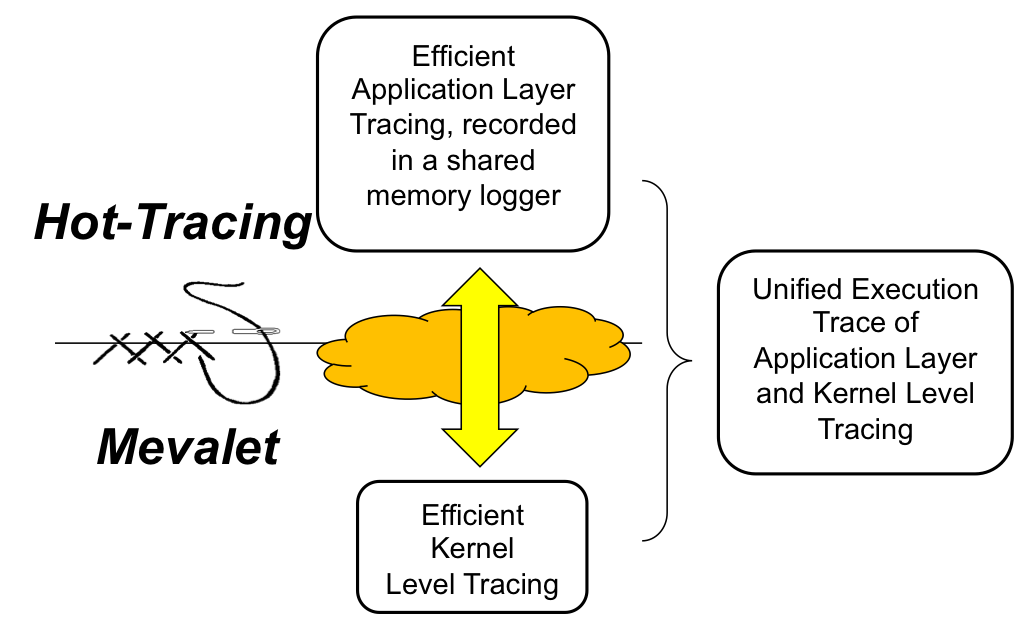
\includegraphics[width=0.5\textwidth]{Images/Dual-Space.eps}
%   \caption{Dual-Space Mechanism}
%   \label{fig:dualspace}
%  \end{center}
% \end{figure}
% 
% 
% iProbe records user-space events in a shared memory user-space logger, simultaneously kernel events are recorded in kernel space using a separate logger called Mevalet \footnote{Mevalet is a proprietary light-weight kernel event logger used in several production environments}. At the end of the recording interval, the log files of both user-space and kernel-space are "stitched" together to get a single execution trace. This avoids any unnecessary context-switches at the production run-time.
% 
% iProbe uses thread local storage to log all events to avoid potential race conditions. To ensure that causal relationships\footnote{theoretically misalignment is possible however to keep a low overhead we have kept a lock-free mechanism} are maintained between kernel traces and user-space traces. iProbe issues dummy system calls which are caught in the kernel log, these are then used along with the time stamps to align both traces into a single unified view.
% 
% When stitching the traces together we use a regression mechanism to align both the traces together.

%iProbe has been built on top of a production level kernel tracer, Mevalet \cite{mevalet}. The key idea behind dual-space architecture is simple, iProbe records user-space events in a shared memory user-space logger. While Kernel Events are recorded using Mevalet a proprietary kernel tracing tool (similar to SystemTap\cite{systemtap}), with a buffered kernel recorder. At the end of the recording interval, the log files of both user-space and kernel-space are stitched together to get a single execution trace. This avoids any unnecessary context-switches at the production run-time.

%iProbe uses rdtsc counters\cite{rdtsc} to measure time along with with the event log, to get a causal order of the events recorded. To ensure that race-conditions do not occur, shared memory logger buffers are maintained by using thread local storage\cite{tls} of every thread. Since events are recorded in a per-thread basis (it is not possible to have race conditions etc.) we assume causal consistency in the event log.  

%Lastly at the end of the recording period iProbe \textbf{stitches} kernel and user-space traces. To ensure that causal relationships are maintained between kernel traces and user-space traces; iProbe issues dummy system calls which are caught as events in the user-space, which are at the same time captured by the kernel space recorders.  At the initiation of every process 4 such system calls are triggered and captured at both user-space and kernel logs. When stitching the traces together we use a regression mechanism to align both the traces together.

% Add how we use regression and anchors to stitch the two together


%\subsection{Dispatcher: Function Selection}

%As described in the previous section, once a function is selected for instrumentation a call is made to the instrumentation by HotPatching. However, there can be potentially a large number of functions belonging to the target binary 

\subsection{Extended iProbe Mode}
\label{sec:advanced}

%Since the default mode of iProbe is compiler driven using instrumentation flags.
As iProbe ColdPatching requires compiler assistance, it is unable to operate on pre-packaged binary applications.
Additionally, compiler flags generally have limited instrumentation flexibility as they generally operate on a programming language abstraction(eg. function calls, loops etc.).
To provide further flexibility, iProbe provides a couple of extended options for ColdPatching of the application

\subsubsection{Static Binary Rewriting Mode} 
 In this mode we use a static binary rewriter to insert instrumentation in a pre-packaged binary. 
Once all functions are instrumented, we use a ColdPatching script to capture all call sites to the instrumentation functions and convert them to \texttt{NOP} instruction.
While this mode allows us to directly operate on binaries, a downside is that our current static binary instrumentation technique also uses mini-trampoline mechanisms. 
As explained in Section \ref{sec:trampoline} static binary rewriters use trampoline based mechanisms which induces minimum two jumps.
In the ColdPatch phase, we convert calls to the instrumentation function to \texttt{NOP}s, however the jmp operations to the trampoline function, and simulation of the overwritten instructions still remain.
The downside of this approach has a small overhead even when instrumentation is turned off.
However, in comparison to pure dynamic instrumentation approach it reduces the time spent in HotPatching.
This is especially important if the number of instrumentation targets is high, and the target binary is large, as it will increase the time taken in analyzing the binaries. 
Additionally, if compiler options cannot be changed for certain sections of the program (plugins/3rd party binaries), iProbe can still be applied using this extended feature.

Our current implementation uses the dyninst \cite{dyninst} and cobi \cite{cobi} to do static instrumentation. 
This allows us to provide the user a configuration file and template which can be used to specify the level of instrumentation (e.g., all entry and exit points for instrumentation), or names of specific target functions, and the instrumentation to be applied to them.
Subsequently in ColdPatch we generate our meta-data list, and use it to HotPatch and apply instrumentation at run-time.

\subsubsection{Developer Driven Macros}
% To provide further flexibility, iProbe provides a developer driven mode using user placed macros as required. 
%For example, compiler based instrumentation is able to insert entry and exit of each function(or other programming abstractions), however at times it may be required to inspect a certain line of code or instruction.
Compiler assisted instrumentation may not provide complete flexibility (usually works on abstractions, such as enter/exit of functions), hence for further flexibility, iProbe provides the user with a header file with calls to macros which can be used to add probe points in the binary.
A call to this macro can be placed as required by the developer. 
The symbol name of the macro is then used in the ColdPatch stage to capture these macros as probe points, and convert them to \texttt{NOP}s.
Since the macros are predefined, they can be safely inserted and interpreted by ColdPatcher.
The HotPatching mechanism is very much the same, using the probe list generated by ColdPatch.

\section{Trampoline vs. Hybrid Approach}
\label{sec:trampoline}

\begin{figure}[h!]
  \begin{center}

    \includegraphics[width=0.95\textwidth]{iprobe/Images/tramp.eps}
    \caption{Traditional Trampoline based Dynamic Instrumentation Mechanisms.}
    \label{fig:tramp}

  \end{center}
\end{figure}

In this section we compare the advantages of our approach compared to traditional trampoline based dynamic instrumentation mechanisms. 
We show the steps followed in trampoline mechanisms, and why our approach has a significant improvement in terms of overhead. 
The basic process of dynamic instrumentation based on trampoline can be divided into 4 steps

\begin{itemize}

\item \textbf{Inspection for Probe Points: } This step inspects and generates a binary patch for the custom instrumentation to be inserted to the target binaries, and find the target probe points which are the code addresses to be modified.

\item \textbf{Memory Allocation for Patching: } Appropriate memory space is allocated for adding the patch and the trampoline code to the target binary.

\item \textbf{Loading and Activation of a Patch: } At run-time the patch is loaded into the target binary, and overwrites the probe point with a jump instruction to a trampoline function and subsequently to the instrumentation function.

\item \textbf{Safety and Reliability Check: } To avoid illegal instructions, it is necessary to check for safety and reliability at the HotPatch stage, and that the logic and correctness of the previous binary remains. 
\end{itemize} 

One of the key reasons for better performance of iProbe as compared to traditional trampoline based designs is the avoidance of multiple jumps enforced in the trampoline mechanism. 
For instance, Figure \ref{fig:tramp} shows the traditional trampoline mechanism used in existing dynamic instrumentation techniques. 
To insert a hook for the function \texttt{foo()}, dynamic instrumentation tools overwrite target probe point instructions with a jump to a small trampoline function (\texttt{jmp()}).
Note that the overwritten code by \texttt{jmp} should be executed somewhere to ensure the correctness of the original program.
The trampoline function executes the overwritten instructions (\texttt{foo fix}) before executing the actual code to be inserted. 
Then this trampoline function in turn makes the call to the instrumentation function (\texttt{foo\_instr}).
Each call instruction can potentially lead to branch mispredictions in the code cache and cause high overhead.
Additionally tools like DTrace, and SystemTap \cite{dtrace,systemtap} have the logger in the kernel space, and cause a context switch in the trampoline using interrupt mechanisms. 

In comparison iProbe has a \texttt{NOP} instruction which can be easily overwritten without resulting in any illegal instructions, and since overwriting is not a problem trampoline function is not required.
This makes the instrumentation process simple resulting in only a single call instruction at all times.

In addition pure binary instrumentation mechanisms need to provide complex guarantees of safety and reliability and hence may lead to further overhead.
Since the patch and trampoline functions overwrite instructions at run-time correctness check must be made at HotPatch time so that an instruction overwrite does not result in an illegal instruction, and that the instructions being patched are not currently being executed.
While this does not enforce a run-time overhead it does enforce a considerable overhead at the HotPatch stage.

Again iProbe avoids this overhead by offloading this process to the compiler stage, and allocating memory ahead of time.


Another important advantage of our hybrid approach as compared to the trampoline approach is that pure dynamic instrumentation techniques are sometimes unable to capture functions from the raw binary. 
This can often be because some compiler optimizations may inherently hide function calls boundaries in the binary. 
A common example of this is \emph{inline functions} where functions are inlined to avoid the creation of a stack frame and concrete calls to these functions. 
This may be done explicitly by the user by defining the function as \emph{inline} or implicitly by the compiler. 
Since our instrumentation uses compiler assisted binary tracing, we are able to use the users definition of functions in the source code to capture entry and exit of functions despite such optimizations.

\section{Implementation}
\label{sec:Implementation}

The design of iProbe is generic and platform agnostic, and works on native binary executables. 
We built a prototype on Linux which is a commonly used platform for service environments. 
In particular, we used a compiler technique based gcc/g++ compiler to implement the hook place holders on standard Linux 32 bit and 64 bit architectures. 
In this section we first show the implementation of the iProbe framework, and then discuss the implementation of FPerf a tool built using iProbe.

\subsection{iProbe Framework}
As we presented in the previous section, the instrumentation procedure consists of two stages.

\indent \textbf{ColdPatch}: In the first phase the place holders for hooks are created in the target binary. 
We implemented this by compiling binaries using the \texttt{-finstrument-functions} flag. 
Note that this can be done simply by appending this flag to the list of compiler flags (e.g., \texttt{CFLAG, CCFLAG, CXXFLAGS}) and most of cases it works without interfering with user code. 

%In details this compiler option places function calls to instrumentation functions (\texttt{\_cyg\_profile\_func\_enter} and \texttt{\_cyg\_profile\_func\_exit})  after the entry and before the exit of every function.
In details this compiler option places function calls to instrumentation functions after the entry and before the exit of every function.
This includes inline functions (see second state in Figure \ref{fig:state_rep}). 
Subsequently, our ColdPatcher uses a binary parser to read through all the target binaries, and search and replace the instruction offsets containing the instrumentation calls with NOP instructions (instruction 90). 
Symbolic and debug information is read from the target binary using commonly available \texttt{objdmp} tools; 
This information combined with target instruction offsets are used to generate the probe list with the following information:
\begin{verbatim}
<Instr Offset, Entry\Exit Point, Meta-Data>
\end{verbatim}
The first field is the instruction offset from the base address, and the second classifies if the target is an entry or an exit point of the function. 
The meta-data here specifies the file, function name, line number etc. 

\indent \textbf{HotPatching}: 
In the run-time phase, we first use the library interposition technique, \texttt{LD\_PRELOAD}, to preload the instrumentation functions in the form of a shared library to the execution environment. 
The HotPatcher then uses a command line interface which interacts with the user and provides the user an option to input the target process and the probe list.
Next, iProbe collects the base addresses of each shared library and the binary connected to the target process from \texttt{/proc/pid/maps}.
The load address and offsets from the probe-list are then used to generate a hash of all possible probing points. 
iProbe then use the meta-data information to provide users a list of target functions and their respective file information.  
It takes as input the list of targets and interrupts the target process. 
We then use \texttt{ptrace} functionality to patch the target instructions with calls to our instrumentation functions, and release the process to execute as normal.
The instrumentation from each function is registered and logged by a shared memory logger. 
To avoid any locking overhead, we have a race free mechanism which
utilizes thread local storage to keep all logs, and a buffered logging mechanism.

\subsection{FPerf: An iProbe Application for Hardware Event Profiling}
\label{sec:imp:configure}


\begin{figure}[t]
    \begin{center}
      \includegraphics[width=0.8\textwidth]{iprobe/Images/sysdesign2.eps}
      \caption{Overview of \textit{FPerf}: Hardware Event Profiler based on iProbe.}
      \label{fig:implement}
    \end{center}
\end{figure}

%In this section we showcase iProbe's strength as a tool building infrastructure.  
We used iProbe to build \emph{FPerf}, an automatic function level hardware event profiler.  
FPerf uses iProbe to provide an automated way to gather hardware performance information at 
application function granularity.
%We used iProbe to build a hardware counter profiling tool called {\em FPerf}.

Hardware counters provide low-overhead access to a wealth of detailed performance information related to CPU's functional units, caches and main memory etc.
Using iProbe's all function profiling, we capture the hardware performance counters at the entry and exit of each function.
%\textit{FPerf} offers fine-grained hardware counter monitor profiling at application function level.
To control the perturbation on applications and the run-time system, \textit{FPerf} also implements a control mechanism to constraint the function profiling overhead within a budget configured by users.

Figure \ref{fig:implement} summarizes \textit{FPerf} implementation. 
It includes a control daemon and an iProbe shared library with customized instrumentation functions. 
The iProbe instrumentation functions access hardware performance counters (using PAPI\cite{papi} in the implementation) at the entry and exit of a selected target function to get the number of hardware events occurring during the function call. 
We define this process as taking one sample. 
Each selected function has a budget quota.
After taking one sample, the instrumentation functions decrease the quota for that application function by one. 
When its quota reaches zero, iProbe does not take sample anymore for that function.


The daemon process controls run-time iProbe profiling through shared memory communication.  
There are two shared data structures for this purpose: a shared control block where the daemon process passes to the iProbe instrumentation functions the profiling quota information, and a shared data table where the iProbe instrumentation functions record the hardware event information for individual function calls. 
When iProbe is enabled, i.e., the binary is HotPatched, daemon periodically collects execution data. 
We limit the total number of samples we want to collect in each time interval to restrict the overhead.  
This limitation is important because in software execution, the function call happens very frequently. 
For example, even with test data size input, the SPEC benchmarks generate 50MB-2GB trace files if we log the records for each function call. 
%Therefore, we initially assign a limitation for the total number of samples to limit the trace log size. 
%In the first 1s, when one function is called; we assign a minimum 1 sample quota for this function. 
%After that, we do not sample other calls to the function. But we keep counting the call number of the function. 
%After the initial 1s, the daemon process assigns the rest total sample quota for each selected application functions proportionally according to the previous call frequency of the functions. 
Functions that are frequently called will get more samples. 
Each selected function cannot take more samples than its assigned quota. 
The only exception happens when one function has never been called before; we assign a minimum one sample quota for each selection function. 
And we pick a function with quota that has not been used up, and decrease the quota of it by one. 
The above overhead control algorithm is a simplified Leaky Bucket algorithm~\cite{lba} originally for traffic shaping in networks. Other overhead control algorithms are also under consideration.

The control daemon also enables/disables the iProbe HotPatching based on user-defined application monitoring rules.
Essentially, this is an external control role on when and what to trace a target application with iProbe.
A full discussion of the hardware event selection scheme and monitoring rule design is beyond the scope of this document. 


\subsection{Safety Checks for iProbe}
\label{sec:safety}

Safety and reliability of the instrumentation technique is a big concern for most run-time instrumentation techniques.
One of the key advantages of iProbe is that because of its hybrid design reliability and correctness issues are handled in a better way inherently.
In this section we discuss how our HotPatch can achieve such properties in details.
%As explained earlier iProbe operates in 3 different modes,(1) compiler-assisted (2) User-macro based, and (3) static binary rewriting.

\indent \textbf{HotPatch check against Illegal instructions}: \quad
Unlike previous techniques iProbe relies on compiler correctness to ensure safety and reliability in its binary mode.
%The resulting instrumented binary in ColdPatch is not only safe but optimized.
To ensure correctness in our ColdPatching phase, we convert call instructions to instrumentation functions with \texttt{NOP} instruction. 
This does not in any way effect the correctness of the binary, except that instrumentation calls are not made. 
To ensure run-time correctness, iProbe uses a safety check when it interrupts the application while HotPatching. 
Our safety check pass ensures that the program counters of all threads belonging to the target applications do not point to the region of code that is being overwritten (i.e. \texttt{NOP} instructions are not overwritten while they are being executed.
This check is similar to those from traditional Ptrace\cite{ptrace} driven debuggers etc \cite{kaho,livepatch,pannus}. 
Here we use the Ptrace \texttt{GETREGS()} call to inspect the program counter, and if it is currently pointing to the target \texttt{NOP} instructions, we allow the execution to move forward before applying the HotPatch. 
Unlike existing trampoline oriented mechanisms iProbe has a small \texttt{NOP} code segments equal to the length of a single call instruction that it overwrites with instrumentation calls, this means that the check can be performed in a fast and efficient manner. 
It is also important to have this check for all threads which share the code-segment, hence the checking must be able to access the process memory map information, and interrupt all the relevant threads.

\indent \textbf{Safe parameter passing to maintain stack consistency}: \quad
An important aspect for instrumentation is the information passed along to the instrumentation function via the parameter values. 
Since the instrumentation calls are defined by the compiler driven instrumentation, the mechanism in which the parameters passed are decided based on the calling convention used by the compiler. \\
Calling conventions can be broadly classified in two types: caller clean-up based, and callee clean-up based. 
In the former the caller is responsible to pop the parameters passed to function, and hence all parameter related stack operations are performed before and after the call instruction inside the code segment of the caller.
In the later however, the callee is responsible to pop the parameters passed to it.
Since parameters are generally passed using the stack it is important to remove them properly to mantain stack consistency. 

To ensure this iProbe enforces that all calls that are made by the static compiler instrumentation must be \emph{cdecl}~\cite{cdecl} calls where the caller performs the cleanup as compared to \emph{std} calls, where the callee performs it. 
%\emph{cdecl} calls push instrumentation parameters before the call, and stack cleanup is also performed by caller function. 
%On the other hand in \emph{std} call convention the stack cleanup is performed by the callee. 
%For simplicity sake, iProbe uses only \emph{cdecl} calls and allows the push and pop operations performed by the caller. 
As the stack cleanup is automatically performed, it maintains stack consistency, and there is a negligible impact in performance due to the redundant stack operations. 
Alternatively for \emph{std} call convention, push instructions could also be converted to \texttt{NOP}s and HotPatched at run-time, we do not do so as a design choice. 

\indent \textbf{Address Space Layout Randomization}: \quad
Another issue that iProbe addresses is ASLR (address space layout randomization), a security measure used in most environments which randomizes the loading address of executables and shared libraries. 
However, since iProbe assumes the full access to the target system, the load addresses are easily available. 
HotPatcher uses the process id of the target to find all load addresses of each binary/shared library and uses them as base offsets to generate correct instruction pointer addresses. 


%\textbf{Developer Driven Macros}
% The developer driven Macros

%\textbf{Static Binary Rewriter}



\section{Evaluation}
\label{sec:eval}

In this section we evaluate various aspects of iProbe. Initially, we show the overhead of iProbe on SPEC CPU 2006 benchmarks\cite{specCPU2006}, we then showcase iProbe vs a normal mode, the binary generated with initial -finstrument-function flag, and the ColdPatched version of the same binary. 
Since iProbe is also geared towards monitoring large scale systems, we also show the overhead of iProbe "ColdPatched" binaries in terms of throughput in apache httpd server, and the mysql database. 
Then we present the overhead for "HotPatching" itself wherein we measure the time taken by iProbe to patch the functions in a live session. Lastly, we compare scalability of iProbe compared to existing state of the art technique SystemTap \cite{systemtap}

\subsection{Overhead of ColdPatch}
The SPEC INT CPU benchmarks 2006 \cite{specCPU2006} is a widely used benchmark in academia, industry and research as relevant representation of real world applications. 
We tested iProbe on 8 benchmark applications shown in Figure \ref{fig:overhead_table}. The first column shows the execution of a normal binary compiled without any instrumentation or debug flags. 
The next column shows the execution time of the corresponding binary compiled using the instrumentation flags (Note here the instrumentation functions are dummy functions). 
Lastly, we show the overhead of a ColdPatched iProbe binary with \texttt{NOP} instead of the call instruction. 
Each benchmark application was executed ten times using SPEC benchmark tools. 
The overhead for a ColdPatched binary was found to be less than five percent for all applications executed, and 0-2 percent for four of the benchmarks. 
The overhead here is basically because of the \texttt{NOP} instructions that are placed in the binary as place-holders for the HotPatching. 
In most non-compute intensive applications (e.g., apache, mysql) we have observed the overhead to be negligible (less than one percent), with no observable effect in terms of throughput. 
Further reduction of the overhead can be achieved by reducing the scope of the functions which are prepared for function tracing by iProbe; for example only using place holders in selected components that need to be further inspected. 
Negligible overhead of ColdPatching process of iProbe shows that applications can be prepared for instrumentation (HotPatching) without adversly effecting the usage of the application.
%Above add details on how components can be selected using -finstrument-functions-execlude-list/ compiler options

%A ColdPatched version of the apache httpd server was tested using the apache ab benchmarking tool, and the overhead was found to be less than 1 percent in throughput. We also ran iProbe on a ColdPatched version of mysql and found similar results. In section.\ref{sec:casestudy_mysql} we further discuss the use of iProbe in a practical debugging case scenario.

%In summary we could observe iProbe having a small to negligible overhead when running a ColdPatched binary. While the overhead of iProbe can be further reduced by using further optimizations in writing the patches, we believe this to be largely an acceptable overhead to enable long term monitoring of applications at the user-level. 


%\begin{table}[h]
%\begin{center}
%    \begin{tabular}{ | l | l | l | l|}
%    \hline
%    Name & Normal & Finstrument & ColdPatch \\ \hline
%    bzip2 & 30.7 & 31.2 & 30.7 \\ \hline
%    sjeng & 13.8 & 15.4 & 14.4 \\ \hline
%    perlbench & 5.24 & 5.49 & 5.24 \\ \hline
%    mcf & 5.98 & 6.72 & 6.28 \\ \hline
%    hmmer & 19.7 & 20 & 19.7  \\ \hline
%    gobmk & 53.4 & 56.6 & 55.5 \\ \hline
%    h264ref & 76.3 & 81 & 80.6 \\ \hline
%    astar & 32.6 & 41.6 & 34.3  \\ \hline
%    \end{tabular}
%\end{center}
%\label{tab:overhead_table}
%\caption{Overhead of iProbe "ColdPatch stage" on SPEC CPU 2006 benchmarks}
%\end{table}


\begin{figure}[h!]
  \begin{center}
    \includegraphics[width=0.8\textwidth]{iprobe/Images/OverheadCold.eps}
    \caption{Overhead of iProbe ``ColdPatch Stage" on SPEC CPU 2006 Benchmarks.}
    \label{fig:overhead_table}
  \end{center}
\end{figure}


\subsection{Overhead of HotPatching and Scalability Analysis}

%One of the advantages of iProbe is that it scales extremely well.
We compared iProbe with UTrace (User Space Tracing in SystemTap) \cite{utrace}, and DynInst \cite{dyninst} on a x86\_64, dual-core machine with Ubuntu 12.10 kernel. 
To test the scalability of these tools, we designed a micro-benchmark and tested the overhead for an increasing amount of events instrumented. 
We instrumented a dummy application with multiple calls to an empty function \texttt{foo}, the instrumentation function in the cases simply increases a global counter for each event triggered (entry and exit of foo). 
Tools were written using all three frameworks to instrument the start and end of the target function and call the instrumentation function. 

Figure \ref{fig:scalability} shows our results when applying iProbe and SystemTap on this micro-benchmark. 
To test the scalability of our the tools, we have increased the number of calls made to \texttt{foo} exponentially (increase by multiples of 10). 
We found that iProbe scales very well and is able to keep the overhead to less than five times for millions of events (10\textsuperscript{8}) generated in less than a second (normal execution) for entry as well as exit of the function. 
While iProbe executed in 1.5 seconds, the overhead observed in SystemTap is around 20 minutes for completion of a subsecond execution, while DynInst takes about 25 seconds. 

As explained in Section \ref{sec:trampoline}, tools such as DynInst use a trampoline mechanism, hence have a minimum of 2 call instructions for each instrumentation.
Additionally SystemTap uses a context switch to switch to the kernel space over and above the traditional trampoline mechanism, resulting in the high overhead, and less scalability observed in our results.

\begin{figure}[h!]
  \begin{center}
    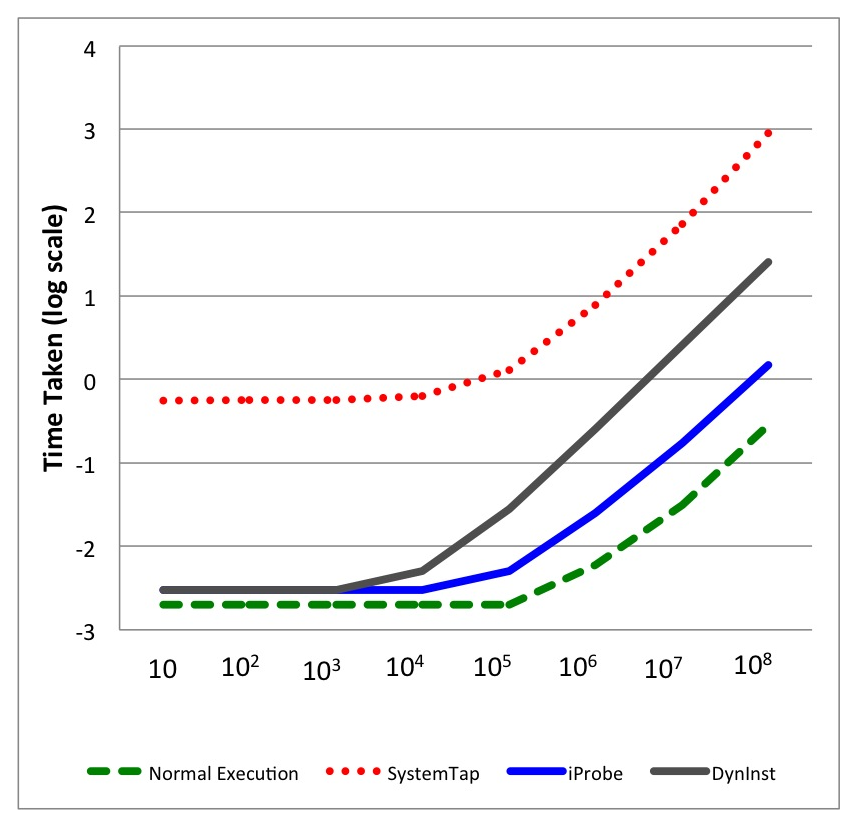
\includegraphics[width=0.8\textwidth]{iprobe/Images/scalability.eps}
    \caption{Overhead and Scalability Comparison of iProbe HotPatching vs. SystemTap vs. DynInst using a Micro-benchmark.}
    \label{fig:scalability}
  \end{center}
\end{figure}

%
%\begin{table}[h]
%\begin{center}
%    \begin{tabular}{ | l | l | l | l|}
%    \hline
%    No. of Events & Normal & SystemTap & iProbe \\ \hline
%    10 & 0.002 & 0.556 & 0.002 \\ \hline
%    10\textsuperscript{2} & 0.002 & 0.566 & 0.003 \\ \hline
%    10\textsuperscript{3} & 0.002 & 0.56 & 0.003 \\ \hline
%   	10\textsuperscript{4} & 0.002 & 0.624 & 0.003 \\ \hline
%    10\textsuperscript{5} & 0.002 & 1.276 & 0.005  \\ \hline
%    10\textsuperscript{6} & 0.007 & 7.805 & 0.025 \\ \hline
%    10\textsuperscript{7} & 0.031 & 72.91 & 0.174 \\ \hline
%    10\textsuperscript{8} & 0.281 & 1200 & 1.502 \\ \hline
%    \end{tabular}
%\end{center}
%    \label{tab:scaling}
%    \caption{A scalability comparison of iProbe vs SystemTap using a micro-benchmark}
%\end{table}


%\begin{table}[h]
%\begin{center}
%    \begin{tabular}{ | l | l | p{2cm} | p{2cm}|}
%    \hline
%    Name & Time & Instrumentation Points & Number of Events \\ \hline
%    bzip2 & 30.7 & 31.2 & 30.7 \\ \hline
%     & 13.8 & 15.4 & 14.4 \\ \hline
%     & 5.24 & 5.49 & 5.24 \\ \hline
%     & 5.98 & 6.72 & 6.28 \\ \hline
%     & 19.5 & 20 & 19.7  \\ \hline
%     & 3.8 & 3.8 & 3.8 \\ \hline
%     & 53.4 & 53.4 & 53.4 \\ \hline
%     & 0.303 & 20 & 19.7  \\ \hline
%     & 76.3 & 3.8 & 3.8 \\ \hline
%     & 1.93 & 53.4 & 53.4 \\ \hline
%     & 30.6 & 20 & 19.7  \\ \hline
%     & 0.936 & 3.8 & 3.8 \\ \hline
%    \end{tabular}
%\end{center}
%\label{tab:RealOverhead}
%\caption{\textbf{Overhead when HotPatching with SPEC CPU 2006 benchmark}}
%\end{table}


\subsection{Case Study: Hardware Event Profiling}
\label{sec:eva}

\subsubsection{Methodology}

%for showcasing iProbe as a framework for new tool development.
%They are all about "automated software engineering" -> "automated dynamic application profiling":
In this section, we present preliminary results on FPerf.
The purpose of this evaluation is for the illustration of iProbe
as a framework for lightweight dynamic application profiling. 
Towards it, we will discuss the results in the context of two FPerf features in hardware event profiling: 
\begin{itemize}
\item \textbf{Instrumentation Automation}: \quad FPerf automates hardware event profiling on massive functions in modern software. This gives a wide and clear view of application performance behaviors.
% This is with the "VTune vs FPerf" results on function coverage, and.  
\item \textbf{Profiling Automation}: \quad FPerf automates the profiling overhead control. This offers a desired monitoring feature for SLA-sensitive production systems. %knob This is with the "budget" results, and 
\end{itemize}
While there are many other important aspects on FPerf to be evaluated such as hardware event information accuracy and different overhead control algorithms, we focus on the above two issues related to iProbe. 

\begin{table}[h!]
\caption{Experiment Platform.}
\label{tab:serverparameter}
\centering
\begin{tabular}{|c|c|}
\hline
\emph{CPU} & Intel Core$^{TM}$ i5-2500 CPU 3.3GHz\\\hline
\emph{OS} & Ubuntu 11.10 \\ \hline
\emph{Kernel} & 3.0.0-12 \\ \hline
\emph{Hardware event} &  \multirow{2}{*}{PAPI 5.1.0} \\ 
\emph{access utility} &  \\ \hline
\emph{Applications} & SPEC CPU2006 \\ \hline
\end{tabular}
\end{table}

Our testbed setup is described in Table \ref{tab:serverparameter}.
The server uses an Intel Core$^{TM}$ i5 CPU running at 3.3GHz, and runs Ubuntu 11.10 Linux with 3.0.0-12 kernel.
FPerf uses PAPI 5.1.0 for hardware performance counter reading, and the traced applications are SPEC CPU2006 benchmarks.

\subsubsection{Instrumentation Automation}

\begin{figure}[h!]
    \begin{center}       
        \epsfig{figure=iprobe/Images/motiv.eps,width=9cm} 
    \end{center}
    \caption{The number of different functions that have been profiled in one execution.}
    \label{fig:motiv}
\end{figure}


Existing profilers featuring hardware events periodically 
(based on time or events) sample the system-wide 
hardware statistics and stitch the hardware
information to running applications (e.g. Intel VTune~\cite{vtune}).
Such sampling based profilers work well to identify and optimize hot code,
but with the possibility of missing 
interesting application functions yet not very hot.
In sharp contrast, \textit{FPerf} is based on iProbe framework, 
it inserts probe functions when entering and exiting each target function.
Therefore, \textit{FPerf} can catch all the function calls in application
execution. In Figure \ref{fig:motiv}, we use VTune and \textit{FPerf} (without budget quota) 
to trace SPEC workloads with test data set. VTune uses all default settings. We find 
that VTune misses certain functions. For example, on {\em 453.povray} VTune only captures 
12 different functions in one execution. In contrast, \textit{FPerf}
does not misses any function because it records data
at enter/exit of each function. Actually, there
are 280 different functions have been used in this execution. 
having the capability to profile all functions or any subset in the program is desirable.
For example, \cite{Jovic:2011} reported that in deployment environment, non-hot functions (i.e.,
functions with low call frequency) might cause performance bugs as well. 

FPerf leverages iProbe's all-function instrumentation and functions-selection utility to achieve instrumentation automation.

\subsubsection{Profiling Automation}

\begin{figure*}[h!]
    \begin{center}
     $\begin{array} {cc}        
        \epsfig{figure=iprobe/Images/slowdownbench.eps,width=7cm} & \epsfig{figure=iprobe/Images/slowdownbase.eps,width=7cm}\\
        \mbox{(a) Slow-down with Overhead Control.} & \mbox{(b) Slow-down with No Overhead Control.}\\
        \epsfig{figure=iprobe/Images/coveragebench.eps,width=7cm} & \epsfig{figure=iprobe/Images/coveragebase.eps,width=7cm}\\
        \mbox{(c) Number of Profiled Functions with Limited Budget.} & \mbox{(d) Number of Profiled Functions with No Budgeting.}\\
        \end{array}$
    \end{center}
    \caption{Overhead Control and Number of Captured Functions Comparison.}
    \label{fig:budgeting}
\end{figure*} 

We tested the measured performance overhead and the number of captured functions of FPerf with different overhead budget. %our budgeting algorithm and compare that with no budgeting case.
As shown in Figure \ref{fig:budgeting}, the Y axis of Figure \ref{fig:budgeting} (a) and (b) is slow-down, which is defined as the execution time with tracing divided by the execution time without tracing. 
The Y axis of Figure \ref{fig:budgeting} (c) and (d) is the number of profiled functions. The ``budget" legend is the total number of samples we assign \textit{FPerf} to take. 
With no budgeting, \textit{FPerf} records hardware counter values at every enter/exit points of each function. 
From Figure \ref{fig:budgeting} (b) and (d), no budgeting can capture all the functions but with large 100x-1000x slow-downs. 
In contrast, FPerf showed its ability to control the performance overhead under $5\%$ in Figure \ref{fig:budgeting} (a).
Of course, FPerf had the possibility to miss functions, as when the budget is too tight, we only sample a limited number of function enter/exit points.

FPerf leverages iProbe's scalability property (predictable low overhead) to achieve the automation on realizing a low and controllable profiling overhead.





%
%\begin{figure*}[t]
%    \begin{center}        
%        \epsfig{figure=Images/correlation.eps,width=15cm}
%    \end{center}
%    \caption{Correlation of collected statistics between budgeting algorithm and no budgeting.}
%    \label{fig:budgetingcorre}
%\end{figure*} 
%
%In the experiment of Fig \ref{fig:budgetingcorre}, we present the correlation coefficient of statistics (performance counter values) between budgeting algorithm and no budgeting cases. In this test, we get the running-average of collected statistics and calculate the correlation coefficient between budgeting cases with no budgeting case. We can observe that, on average, the budgeting algorithm collected statistics have very high correlation coefficient with no budgeting case. However, for certain workload (e.g., soplex), since \textit{FPerf} skips a lot functions (we can tell that from comparing Fig \ref{fig:budgeting} c and d), there is a large difference between budgeting and no budgeting cases.
%

%\section{Related Work}
\label{sec:related}

 %iProbe is motivated by existing production monitoring tools such as dtrace\cite{dtrace,lttng,systemtap}, and dynamic instrumentation available in several kernels. While iProbe does not focus on providing a very declarative query language or methodology, we have instead combined these approaches with compiler instrumentation mechanisms which can be applied using most compiler frameworks using either existing flags or analysis tools such as LLVM\cite{llvm}, gimple\cite{gimple}, or rose\cite{rose}. 
 
\begin{figure*}[ht]
  \begin{center}
  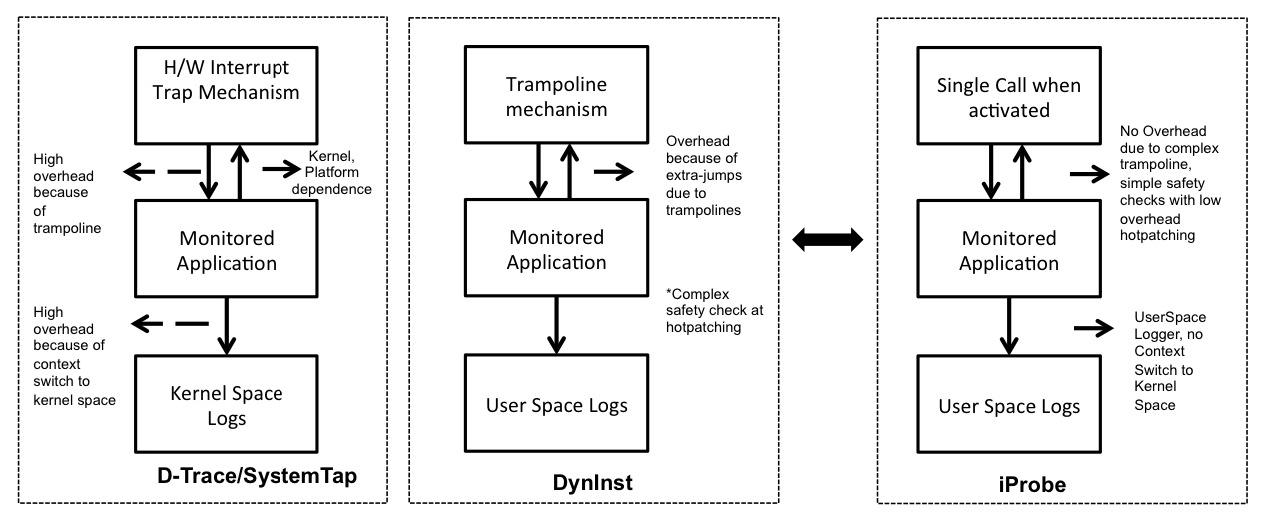
\includegraphics[width=0.9\textwidth]{iprobe/Images/related.eps}
  \caption{Advantages of iProbe over existing monitoring frameworks DTrace/SystemTap and DynInst}
  \label{fig:related}
 \end{center}
\end{figure*}

\noindent \textbf{Source Code or Compiler Instrumentation Mechanisms}: \quad
 Source code instrumentation is one of the most widely available mechanisms for monitoring. 
 In essence, users can insert debug statements with runtime flags to dump and inspect program status with varying verbosity levels. 
 The log4j~\cite{log4j} and log4c~\cite{log4c} frameworks are commonly used libraries to perform program tracing in many open source projects in the source code level. 
 Additionally compilers have several inbuilt profilers which can be used along with tools such as gprof and jprof to gather statistics about program execution.
 While source code techniques allow very light weight instrumentation, by design they are static and can only be changed at the start of application execution. 
 iProbe on the other hand offers run-time instrumentation that allows dynamic decisions on tracing with comparable overhead.


\noindent \textbf{Run-time Instrumentation Mechanisms}: \quad
There are several kernel level tracing tools such as DTrace, LTTng, SystemTap \cite{dtrace,lttng,systemtap} developed by researchers over the years.
iProbe differs from these approaches mainly in two ways: Firstly, all of these approaches use a technique similar to software interrupt to switch to kernel space and generate a log event by overwriting the target instructions. 
They then execute the instrumentation code, and either generate a trampoline mechanism or re-execute the overwritten target instructions and then jump back to the subsequent instructions. 
As shown in Figure.\ref{fig:related} this introduces context-switches between user-space and the kernel, causing needless overhead. 
iProbe avoids this overhead by having a completely user-space based design.
Secondly, all these approaches require to perform complex checks for correctness which can cause unnecessary overhead at both hotpatching, and when running an instrumented binary. 
%debug information at run-time to find the target function requested by the user. This requirement may not be met in production binaries, and iProbe does not require it in the binaries.

Fay \cite{fay} is a platform-dependent approach which uses the empty spaces at the start of the functions available in Windows binaries for instrumentation. 
To ensure the capture of the entry and exit of functions, Fay calls the target function within its instrumentation thereby introducing an extra stack frame for each target instrumentation. 
This operation is similar to a mini-trampoline and hence incurs an overhead. 
Fay logs function execution in the kernel space and hence also has a context-switch overhead.
iProbe avoids such overhead by introducing markers at the beginning and end of
each function using a 

Another well known tool is DynInst\cite{dyninst}. This tool provides a rich dynamic instrumentation capability and has pure back box solution towards instrumentation of any application.
However, as shown in Figure.\ref{fig:related} it is also based on traditional trampoline mechanisms, and induces a high overhead because of unnecessary jump instructions.
Additionally it can have higher overhead because of complex security checks. 
Other similar trampoline based tools like kaho and pannus\cite{pannus,kaho} have also been proposed, but they focus more towards patching binaries to add \emph{fixes} to correct a bug.
 
% platform independent 
%compiler technique.

\noindent \textbf{Debuggers}: \quad
Instrumentation is a commonly used technique in debugging. Many debuggers such as gdb \cite{gdb} and Eclipse have breakpoints and watchpoints which can stop the execution of programs and inspect program conditions. These features are based on various techniques including \texttt{ptrace} and hardware debugging support (single step mode and debug registers). While they provide such powerful instrumentation capabilities, there are in general not adequate for beyond the debugging purposes due to overwhelming overhead.

\noindent \textbf{Dynamic Translation Tools}: \quad
Software engineering communities have been using dynamic translation tools such as Pin \cite{pin} and Valgrind \cite{valgrind} to inspect program characteristics. 
These tools dynamically translate program code before execution and allow users to insert custom instrumentation code flexibly. They are capable to instrument non-debug binaries and provide versatile tools such as memory checkers and program profilers. However, similar to debuggers, they are generally considered as debugging tools and their overhead is significantly higher than runtime tracers.



\section{Summary}
\label{sec:iProbeSummary}

Flexibility and performance have been two conflicting goals 
for the design of dynamic instrumentation tools.
iProbe offers a solution to this problem by using a two-stage process that offloads much of the complexity involved in run-time instrumentation to an offline stage. 
It provides a dynamic application profiling framework
to allow for easy and pervasive instrumentation of application functions
and selective activation. 
We presented in the evaluation that iProbe is significantly faster than existing state-of-the-art tools, and scales well in large application software.

%It is applicable to both user and kernel event tracing. It can be utilized using 
%a simple GUI interface which reads all instrumentable functions in a binary. 
%iProbe provides for packaging a monitoring system to be deployed with the target application.
%It provides a system to inves tigate performance pathologies, or reliability 
%problems in target binary applications. It has been tested on Linux 32 and 64bit 
%applications.



\part{Applications of Live Debugging}
\chapter{Active Debugging and Applications of Live Debugging}
\label{ch:activedebugging}

\section{Overview}
\label{sec:guided_overview}

In the sections until now, we have introduced a framework for \livedebugging, a tool for pre-packaging binaries to make them \livedebugging friendly. 
We now discuss some applications of \livedebugging in the real-world, and in particular introduce a new mechanism called \activedebugging.


The debug container allows for debuggers to apply any ad-hoc technique used in offline debugging.
However, in order for us to have continuous debugging, it is essential to allow for forward progress in the debug container. 
Furthermore, the divergence due to instrumentation should not stop forward-progress in the debug-container.
%Having a debug-container which is isolated from the production, but still in sync with production services, allows a variety of ad-hoc debugging approaches to be integrated and leverage our framework.
Traditional offline debugging approaches, such as dynamic instrumentation can be easily directly applied to the debug-container at a much higher granularity than would be allowed in normal production services. 
Others like memory or performance profiling, and execution traces can also be applied in the debug container.
Similarly the \debugcontainer can be used as a staging mechanism for record-replay on demand to ensure deterministic execution.
It is essential however, that none of them functionally modifies the application or else manages any modifications introduced such that forward progress is possible.

This chapter is divided in the following key parts: Firstly, in section~\ref{sec:guidedDiscussion}, we discuss the advantages and limitations of \parikshan in real-world settings.
We highlight certain key points that the debugger most be aware of when debugging applications with \parikshan, so that he can do reliable and fast debugging. 
In section~\ref{sec:activeDebuggingScenarios}, we classify debugging production applications in two high level debugging scenario categories: \emph{post-facto}, and \emph{proactive} analysis.
We leverage these classifications to explain how different techniques can be applied in \parikshan, and in which scenarios debugging on the fly does not make sense.
Next we list some existing debugging technologies, like statistical debugging, execution tracing, record and replay etc. to explain how they can be either directly applied or modified slightly and applied with the \parikshan framework to significantly improve their analysis.

In the next section we introduce budget-limited adaptive instrumentation. Which focuses further on how to allow for continuous debugging with the maximum information gain.
One of the key criteria for successful statistical debugging is to have higher instrumentation rates, to make the results more statistically significant. 
There is a clear trade-off between instrumentation vs performance overhead for statistical instrumentation. 
A key advantage of using this with \parikshan is that we can provide live feedback based buffer size and bounded overheads, hence squeezing the maximum advantage out of statistical debugging without impacting the overhead. 
We evaluate the slack available in each request for instrumentation without risking a buffer overflow and getting out of sync of the production container.
%Live interactive debugging provided by \parikshan further allows for quick updates to the instrumentation and targeting specific areas of the application code.
Budget limited instrumentation is inspired from statistical debugging~\cite{statisticalDebugging}, and focuses on a two-pronged goal of bounding the instrumentation overhead to avoid buffer overflows in \parikshan, and simultaneously have maximum feedback regarding information gained from real-time instrumentation.

In the last section, we introduce \activedebugging whereby developers can apply a patch/fix or apply a test in the \debugcontainer.
\activedebugging ensures that any modifications in the \debugcontainer does not lead to a state change in the \productioncontainer.
This will enable the debugger to fix/patch or run test-cases in the debug-container while ensuring forward progress and in sync with production. 
We are inspired from existing perpetual invivo testing frameworks like INVITE~\cite{invivo}(which also provides partial test-isolation), in the production environment.
We currently restrict \active debugging to patches/and test-cases only bring about local changes, and not global changes in the application.



\xxx{This section is divided in the 3 parts: First in section, next in section, next in section, }

\iffalse
One possible route that we wish to explore further is how to allow for validation of test-cases, or validate functional patches/fixes, which may modify the output.
For the purposes of our exploration, we have currently assumed that these patches/and test-cases only bring about local changes, and not global changes in the application.
In this section, we introduce the concept of \activedebugging, whereby developers can apply a patch/fix or apply a test in the \debugcontainer.
\activedebugging ensures that any modifications in the \debugcontainer does not lead to a state change in the \productioncontainer.
This will enable the debugger to fix/patch or run test-cases in the debug-container while ensuring forward progress and in sync with production. 
We are inspired from existing perpetual invivo testing frameworks like INVITE~\cite{invivo}(which also provides partial test-isolation), in the production environment.

In recent years several monitoring techniques have been developed to monitor the health of production systems.
For example most modern operating systems have resource monitors~\cite{linuxHealth, windowsHealth, macHealth}, which can be used to track the CPU, memory usage, cache misses, temperature etc. of the physical machine.
These are useful to discover high workloads, or if the machine is stressed because of heavy resource usage.
Similarly, application level monitoring tools are used to report transactions or errors in the application.
Monitoring outputs usually provide the first clue towards resolving an error in the debugging process.
%While useful, these monitoring mechanisms  have a performance trade-off with the amount of instrumentation that can be done.
%Furthermore, the information provided by these logs may not be enough to understand the root-cause of the error.

However all monitoring/instrumentation techniques impose a performance overhead on the applications.
This can adversely impact user-experience, hence real-world production instrumentation is generally kept at very low levels.
\parikshan provides an alternative mechanism where this debugging/instrumentation can be done in parallel on a sandboxed cloned container.
Any instrumentation or monitoring in the debug-container has no performance impact on the production container.
In the context of our system, debuggers can use a variety of ad-hoc approaches to capture the root-cause of an error.
For example a naive approach could be to use trial-and-error instrumentation to find the execution trace for the error.
Alternatively, the user could also do aggressive brute force instrumentation for all function execution, which could help locate the problem.
However, both these approaches can have potentially high overheads, which in turn can lead to a buffer overflow.

In this chapter we introduce a statistical sampling approach which imposes a bounded performance overhead, to ensure maximal live debugging information, without causing a buffer overflow.
%In our search for more systematic approach towards live debugging, we looked towards two possible techniques.
%Firstly, we try to implement an automated budget limited instrumentation approach for capturing application logs.
We are inspired by previous work done in statistical debugging~\cite{cbi}, and delta debugging~\cite{delta} techniques which aim to streamline and automate the process of bug localization.
This is achieved by having predicate profiles from both successful and failing runs of a program and applying statistical techniques to pinpoint the cause of the failure.
The core advantage of statistical debugging is that the sampling frequency of the instrumentation can be decreased to reduce the instrumentation overhead.

One of the key criteria for successful statistical debugging is to have higher instrumentation rates, to make the results more statistically significant. 
There is a clear trade-off between instrumentation vs performance overhead for statistical instrumentation. 
A key advantage of using this with \parikshan is that we can provide live feedback based buffer size and bounded overheads, hence squeezing the maximum advantage out of statistical debugging without impacting the overhead. 
We evaluate the slack available in each request for instrumentation without risking a buffer overflow and getting out of sync of the production container.
Live interactive debugging provided by \parikshan further allows for quick updates to the instrumentation and targeting specific areas of the application code.
\fi

\section{Live Debugging using Parikshan}
\label{sec:guidedDiscussion}

The following are some key advantages of \parikshan that can be leveraged for debugging user-facing applications on the fly:

\begin{itemize}
	
	\item \textbf{Sandboxed Environment}: The debug container runs in a sandboxed environment which is running in parallel to the real production system, but any changes in the \debugcontainer are not reflected to the end-user. This is a key advantage in several debugging techniques which are disruptive, and can change the final output. 
	
	Normal debugging mechanisms such as triggering a breakpoints or patching in a new exception/assertion to figure out if a particular ``condition" in the application system state is breaking the code, cannot be done in a production code as it could lead to a critical system crash. On the other hand, \parikshan's debug containers are ideal for this scenario as they will allow developers to put in a patches without any fear of system failure.
	
	\item \textbf{Zero Overhead Monitoring}:The most novel aspect of \parikshan is that it allows for zero overhead monitoring of the production system. This means that high-overhead debugging techniques can be applied on the debug-container without incurring a slow-down in production.
	
	Debugging techniques like record-replay tools which have traditionally high recording overheads can generally not be applied in production systems. However, \parikshan can be used to decouple the recording overhead from production, and can allow for relatively higher overhead recording with more granularity.
	
	\item \textbf{Capturing production system state}:
	One of the key factors behind capturing the root-cause of any bug is to capture the system state in which it was triggered. \parikshan has a live-cloning facility that clones the system state and creates a replica of the production. Assuming that the bug was triggered in the production, the replica captures the same state as the production container.
	
	\item \textbf{Compartmentalizing large-scale systems context}:
	Most real-world services are deployed using a combination of several SOA applications, each of them interacting together to provide an end-to-end service. This could be a traditional 3 tier commerce system, with an application layer, a database layer and a web front-end, or a more scaled out social media system with compute services, recommendation engines, short term queuing systems as well as storage and database layers. 
	Bugs in such distributed systems are particularly difficult to re-create as they require the entire large-scale system to be re-created in order to trigger the bug. 
	Traditional record-replay systems if used are insufficient as they are usually focused on a small subset of applications.
	
	Since, our framework leverages network duplication, \parikshan can allow looking at applications in isolation and capturing the system state as well as the input of the running application, without having to re-create the entire buggy infrastructure. 
	In a complex multi-tier system this is a very useful advantage to localize the bug.
	
	
\end{itemize}

At the same time there are some things that the administrator must be aware of

\begin{itemize}
	\item \textbf{Continuous Debugging and Forward Progress}:
	%\livedebugging allows users to debug applications on-the-fly. 
	The debug-container where one can do debugging runs in parallel to the production container. This is done by first making a live replica of the system followed by duplicating and sending the network input to the \debugcontainer. 
	In a way the \debugcontainer still communicates with the entire system although it's responses are dropped. 
	To ensure forward progress in the \debugcontainer, it is essential that the \debugcontainer is in-sync with the production container, so that the responses, and the requests from the network are the expected responses for forward progress in the application running on the \debugcontainer.
	
	Take for instance, a MySQL~\cite{mysql} service running in the \productioncontainer and \debugcontainer. If during our debugging efforts we modify the state of the debug service such that the MySQL database is no longer in synch with the production service, then any future communication from the network could lead to the state of the debug-container to further diverge from the production. Additionally, depending on the incoming requests or responses the debug application may crash or not have any forward progress.
	
	No forward-progress does not necessarily mean that debugging cannot take place, however for continuous debugging to take place, once the machine has crashed it needs to be re-cloned from the production container, for further debugging. Further, given programmer knowledge the debugger can try his best to avoid state changes that would lead to an un-intentional crash.
	
	\item \textbf{Debug Window}:
	As explained earlier, most debugging mechanisms generally requires instrumentation and tracking execution flow. This means that the application will spend some compute cycles in logging instrumentation points thereby having a slow-down. While \parikshan avoids any slow-down in the production environment, there will be some slow-down in the debug-container. 
	
	The amount of time till which the production container remains in synch with the \debugcontainer is called the debug-window(see section~\ref{sec:parikshanWindow}). The window time depends on the overhead, the size of the buffer and the incoming request rate. If a buffer overflow happens because the debug-window has finished, the \debugcontainer needs to be re-synced with the production container.
	
	In our experiments, we have observed, that \parikshan is able to accommodate significant overhead without incurring a buffer overflow.	
	Administrators or debuggers using \parikshan should keep the overhead of their instrumentation in mind when debugging in \parikshan. Of-course they can always re-clone the \productioncontainer to start a new debugging session.
	
	\item \textbf{Non-determinism}:
	
	One of the most difficult bugs to localize are non-deterministic bugs. While \parikshan is able to capture system non-determinism by capturing the input, it is unable to capture thread non-determinism. Most service-oriented applications have a large number of threads/processes, which means that different threading schedules can happen in the production container as compared to the debug-container.
	This means, that a specific ordering of events that caused a bug to be triggered in the production container, may not happen in the debug-container.
	
	There are multiple ways that this problem can be looked at. Firstly, while it's difficult to quantify, for all the non-deterministic cases in our case-studies, we were able to trigger the bug in both the production and the replica. 
	In the case where the bug is actually triggered in the \debugcontainer, the debugging can take place as usual for other other bugs.
	If that is not the case, there are several techniques which provide systematic ``search" for different threading schedules based on a high granularity recording of all potential thread synchronization points, and read/write threads. While such high granularity recording is not possible in the production container, it can definitely be done in the \debugcontainer without any impact on the production service.
	
\end{itemize}

\section{Debugging Scenarios}
\label{sec:activeDebuggingScenarios}

Based on our case-studies, and survey of commonly seen SOA bugs we classify the following scenarios for live debugging. 
In each of the scenarios we explain how different categories of bugs can be caught or analyzed.

\subsection{Scenario 1: Post-Facto Analysis}
\label{sec:activePostFactoAnalysis}

In this scenario, the error/fault happens without \livedebugging having been turned on i.e. the service is only running in the production container, and there is no replica.
Typically light-weight instrumentation or monitoring is always turned on in all service/transaction systems. 
Such monitoring systems are very limited in their capabilities to localize the bug, but they can indicate if the system is in a faulty state.

For our post-facto analysis, we use such monitoring systems as a trigger to start \livedebugging once faulty behavior is detected. 
The advantage of such an approach is that debugging resources are only used on-demand, and in an otherwise normal system only the \productioncontainer is utilizing the resources.


There are three kind of bugs that can be considered in this kind of situation:

\begin{itemize}
	
	\item \textbf{Persistent Stateless Bugs}: 
	
	This is the ideal scenario for \parikshan.
	Persistent bugs are those that persist in the application and are long running. 
	They can impact either some or all the requests in a SOA application.
	Common examples of such bugs are memory leak, performance slow-down, semantic bugs among others.
	Assuming they are statistically significant, persistent bugs will be triggered again and again by different requests.
	
	We define \emph{stateless bugs} here as bugs which do not impact the state of the system, hence not impacting future queries. 
	For instance read only operations in the database are stateless, however a write operation which corrupts or modifies the database is stateful, and is likely to impact and cause errors in future transactions.
	
	Hence, such bugs are only dependent on the current system state, and the incoming network input.
	Once such a bug is detected in the production system, \parikshan can initiate a live cloning process and create a replica for debugging purposes. 
	Assuming similar inputs which can trigger the bug are sent by the user, the bug can be observed and debugged the \debugcontainer.
	
	\item \textbf{Persistent Stateful Bugs}:
	
	Stateful bugs are those bugs which can impact the state and change it such that any such bug impacts future transactions in the production container as well.
	For instance in a database service a table may have been corrupted, or it's state changed so that certain transactions are permanently impacted. 
	While having the execution trace of the initial request which triggered a faulty state is useful, the ability to analyze the current state of the application is also extremely useful in localizing the error.
	
	Creating a live clone after such an error and checking the responses state of future impacted transaction, as well as the current state of the database can be a good starting point towards resolving the error. 
	
	\item \textbf{Crashing Bugs}: 
	
	Crashing bugs are bugs that lead to a crash in the system thereby stopping the service.
	Unhandled exceptions, or system traps are generally the cause of such crashes.
	Unfortunately \parikshan has limited utilization for post-facto analysis of a crashing bug. 
	Since \parikshan is not turned ``on" at the time of the crash, any post-facto analysis for creating a \debugcontainer is not possible.

	
\end{itemize} 

\subsection{Scenario 2: Proactive Analysis}
\label{sec:activeProactiveAnalysis}

Proactive analysis are scenarios where the user starts debugging when the system is performing normally and their is no bug. This is the same as having instrumentation on or monitoring a production server, except that in this case the instrumentation is actually present in the \debugcontainer.

One possible scenario is to use the \debugcontainer to do recording or high granularity instrumentation. This is extremely useful feature to have if you expect to have higher overheads of instrumentation, which are unacceptable in the production environment. 
On the other hand our \debugcontainer can have much higher instrumentation without any performance penalty on the production container.
Another useful feature of staged recording is the case where the debugger needs to put in breakpoints or potentially instrumentation which can cause the system to crash can also be put in the \debugcontainer
Proactive recording is basically use to track bugs that could happen in the future as the transaction or request which causes the failure is caught as well, as well as it is caught in the context of the system state. 
Once a bug is caught, the cause can be independently explored in the \debugcontainer.

Proactive Analysis, is useful for both stateless and stateful bugs, we do not differentiate between them here as even in the case of a stateful bug, debugging is always turned on. 
Proactive approaches can be compared to existing approaches like statistical debugging~\cite{statisticalDebugging} which use active statistical profiling to compare between successful and buggy runs, to isolate the problem. We discuss statistical debugging in section~\ref{sec:activeStatisticalDebugging} and present an advanced approach based on the same in section~\ref{sec:activeBudgetLimited}.
Other proactive body of work include record-replay infrastructures, which record production systems, and can replay the execution if a bug is discovered.
In section~\ref{sec:activeStagedRecordReplay}, we have discussed staged record-and-replay, which is an advanced record-replay technique that can be applied with the help of \parikshan.



\section{Existing Debugging Mechanisms and Applications}
\label{sec:activeExistingTechniques}

\subsection{Execution Tracing}
\label{sec:activeExecutionTracing}

One of the most common techniques to debug any application is execution tracing. 
Execution tracing gives a trace log of all the functions/modules executed when an input is received. 
This helps the debugger in looking at only those execution points and makes it easier to reason out what is going wrong.

Execution tracing can happen at different granularity: for instance an application can be monitored at function level granularity (only entry and exit of function is monitored), or for deeper understanding at read/write, synchronization point or even instruction level granularity.
Depending on how much granularity the tracing is done at the overhead may be unacceptable for production systems.

Execution tracing can be de-coupled from original execution and put in \debugcontainer for higher granularity instrumentation. 
Such techniques which decouple execution and analysis also been previously explored in papers like Aftersight~\cite{aftersight} and DoublePlay~\cite{doubleplay}.
\parikshan provides a systematic framework for decoupling without enforcing strong constraints on the user.

\subsection{Statistical Debugging}
\label{sec:activeStatisticalDebugging}

Statistical debugging aims to automate the process of isolating bugs by profiling several runs of the program and using statistical analysis to pinpoint the likely causes of failure. 
The seminal paper on statistical debugging~\cite{statisticalDebugging}, has lead to several advanced approaches~\cite{holmes,adaptive,statisticalPerformance}, and is now a well established debugging methedology. 

The core mechanism of statistical debugging is to have probabilistic profiling, by sampling execution points and comparing the execution traces for failed and successful transactions.
It then uses statistical models to identify path profiles that are strongly predictive of failure. 
This can be used to iteratively localize the bug causing execution, and can then be manually analyzed by \parikshan.

The core advantage of statistical testing is that the sampling frequency of the instrumentation can be decreased to reduce the instrumentation overhead.
However, the instrumentation frequency for such testing to be successful needs to be statistically significant. 
Unfortunately, overhead concerns in the production environment limit the frequency of instrumentation.
In \parikshan, the buffer utilization can be used to control the frequency of such statistical instrumentation in the debug-container. 
This would allow the user to utilize the slack available in the debug-container for instrumentation to it's maximum, without leading to an overflow. 
Thereby improving the efficiency of statistical testing.

Statistical debugging is one of the systematic bug localization approaches that can be directly applied in the \debugcontainer, with the added advantage that the amount of instrumentation that can be applied in the debug-container is much higher than production containers. 
Apart from regular semantic bugs, previous body of works have shown that statistical debugging is useful in detecting a variety of other bugs like concurrency bugs~\cite{statisticalConcurrency}, and performance~\cite{statisticalPerformance}.

\subsection{Staging Record and Replay}
\label{sec:activeStagedRecordReplay}

\begin{figure}[h!]
	
	\centering
	\includegraphics[width=0.99\textwidth]{guided/figs/stagedRecordReplay.pdf}
	\caption{Staged Record and Replay using \parikshan}
	\label{fig:stagedRecordReplay}
\end{figure}

One well known sub-category of debugging service-oriented applications are record-replay infrastructures.
In the past decade there have been numerous record-and-replay infrastructures which have been introduced in academia.
The core focus of these techniques is to faithfully reproduce the execution trace and allow for offline debugging.
However, in order faithfully reproduce the exact same instrumentation, the recording phase must record a higher granularity of execution.
Unfortunately, this means a higher overhead at the time of recording in the production system.
Such recording overhead is usually unacceptable in most production systems.

Record and replay can be coupled with the \debugcontainer to avoid any overhead on the \productioncontainer.
This is done by staging the recording for record-and-replay in the \debugcontainer instead of the production, and then replaying that for offline analysis.
In figure~\ref{fig:stagedRecordReplay} we show how the production system can first be ``live-cloned". A copy of the container's image can be stored/retained for future offline replay - this incurs no extra overhead as taking a live snapshot is a part of the live-cloning process. Recording can then be started on the \debugcontainer, and logs collected here can be used to do offline replay.

An important aspect to remember here is that \textbf{non-determinism} can lead to different execution flows (with low probability as the system is a clone of the original) in the \debugcontainer v.s. the \productioncontainer.
Hence simply replaying an execution trace in the \debugcontainer, may not lead to the same execution which triggers the bug.
However several existing record-and-replay techniques offer search capabilities to replay and search through all possible concurrent schedules which could have triggered a non-deterministic error.
Hence we propose that the exact executing schedule which triggered a bug, and using the \debugcontainer for recording instead of the \productioncontainer is a viable alternative to traditional record-replay techniques.

\subsection{A-B Testing}

\begin{figure}[h!]
	
	\centering
	\includegraphics[width=0.99\textwidth]{guided/figs/ABTesting.pdf}
	\caption{Traditional A-B Testing}
	\label{fig:abTesting}
\end{figure}

A/B testing (sometimes called split testing) is comparing two versions of a web page to see which one performs better. 
You compare two web pages by showing the two variants (let's call them A and B) to similar visitors at the same time.
Uer operations in A can then be compared to user scenario's in B to understand which is better, and how well it was received.

Similar A/B Testing, for performance patches or other functional patches, can be done in the \debugcontainer for evaluation of patches which are functionally similar and have same input/output.


\subsection{Interactive Debugging}

The most common debugging tools used in the development environment are interactive debuggers. 
Debugging tools like gdb~\cite{gdb}, pdb, or eclipse~\cite{eclipse}, provide intelligent debugging options for doing interactive debugging. 
This includes adding breakpoints, watch-points, stack-unrolling etc.
The downside to all of these techniques is that they essentially stop the service or execution.
Once a process has been attached to a debugger, a shadow process in also attached to it and the rest of the execution follows with just-in-time execution, allowing the debugger to monitor the progress step-by-step therefore making it substantially easier to catch the error.
Unfortunately, this cannot be applied to the \productioncontainer.

However this can be easily applied towards the \debugcontainer, where the execution trace can be observed once a breakpoint has been reached.
While this does mean that the replica will not be able to service any more requests (except for those that have been buffered), the request which is inside the breakpoint will be processed.
Generally breakpoint and step-by-step execution monitoring is used for a limited scope of execution within a single transaction.
Once, finished future transactions can also be debugged after doing a re-sync by applying live cloning again.

\subsection{Fault Tolerance Testing}

One of the places that \parikshan can be applied is for fault tolerance testing.
To motivate this let us look at Netflix's current testing model.
Netflix has a suite of real-time techniques~\cite{chaosengineering} for testing fault-tolerance of it's systems.
Amongst them, chief is chaos monkey~\cite{chaosmonkey}, which uses fault injection in real production systems to do fault tolerance testing.
It randomly injects time-outs, resource hogs etc. in production systems. 
This allows Netflix to test the robustness of their system at scale, and avoid large-scale system crashes. 
The motivation behind this approach is that it's nearly impossible to create a large-size test-bed to have a realistic fault tolerance testing for the scale of machines that Netflix has. 
Chaos Monkey allows Netflix to do it's fault tolerance testing at a small cost to the customer experience, while avoiding fatal crashes which could lead to longer downtimes.
The obvious downside of this approach is that the service becomes temporarily unavailable and re-sets, or forces a slow-down on the end-user experience (this may or may not be visible to the user). 

Since \parikshan can be run in a live system, it can capture the scale of a large-system, and can allow users to test for faults in an isolated environment.
The only limitation being that the fault-injections should be such that the impact of these faults can be isolated to targeted systems, or a sub-domain of a network which has been cloned, and the tolerance built into the system can be tested (it would be too expensive to clone the entire deployment).


\section{Budget Limited, Adaptive Instrumentation}
\label{sec:activeBudgetLimited}

As explained in section~\ref{sec:parikshanDesign}, the asynchronous packet forwarding in our network duplication results in a \debugwindow.
The \debugwindow is the time before the buffer of the debug-container overflows because of the input from the user.
The TCP connection from end-users to production-containers are synchronized by default.
This means that the rate of incoming packets is limited by the amount of packets that can be processed by the production container.
On the other hand, packets are forwarded asynchronously to an internal-buffer in the debug-container.
The duration of the \debugwindow is dependent on the incoming workload, the size of the buffer, and the overhead/slowdown caused due to instrumentation in the debug-container.
Each time the buffer is filled, requests are dropped, and the debug-container can get out of sync with the production container.
To get the debug-container back in sync, the container needs to be re-cloned.
While duplicating the requests has negligible impact on the production container, cloning the production container can incur a small suspend time(workload dependent).
\iffalse
\begin{wrapfigure}{R}{0.75\textwidth}
	\centering
	\includegraphics[width=0.45\textwidth]{queue/figs/queue.pdf}
	\caption{\label{fig:queueModel}An example of a simple queue applied to a SOA application. Here the arrival rate of the requests to the queue is a poisson process with rate $\lambda$, and the service time of each request is a poisson process with rate $\mu$. In the default SOA settings, the client request is being sent into a blocking TCP queue, where the incoming requests are rate limited by $\mu$. Hence, there is never any buffer overflow}
\end{wrapfigure}
\fi

The duration of the \debugwindow can be increased by reducing the instrumentation.
At the same time we wish to increase the maximum information that can be gained out of the instrumentation to do an effective bug diagnosis.
Essentially for a given buffer size and workload, there is a trade-off between the information gain due to more instrumentation and the duration of the \debugwindow.
Hence our general objective is to increase the information gain through instrumentation while avoiding a buffer overflow.

We divide this task into  pro-active and re-active approaches which can complement each other. Firstly, we pro-actively assign budgets using queuing theory and simulations. We try to find that assuming a poisson distribution for average processing time of each request and the inter-arrival time of requests, we can find expected buffer sizes for a reasonable debug-window length. Secondly, we propose a re-active mechanism triggered by the amount of buffer used. The buffer utilization can be continuously monitored and the instrumentation sampling can be exponentially reduced if the buffer is near capacity. This can be combined with statistical debugging to have the maximum information gain possible. 

\subsection{Proactive: Modeling Budgets}
\label{sec:activeProactiveModeling}


\begin{figure}[t!]

		\centering
		\includegraphics[width=0.7\textwidth]{queue/figs/queue.pdf}
		\caption{\parikshan applied to a mid-tier service}
		\label{fig:queueModel}
\end{figure}
\begin{figure}
		\centering
		\includegraphics[width=0.99\textwidth]{queue/figs/queueCloned.pdf}
		\caption{External and Internal Mode for live cloning: P1 is the production, and D1 is the debug container.}
		\label{fig:queueClonedModel}
\end{figure}
	
%\caption{Modeling \livedebugging using queuing theory}
%\end{figure*}

\iffalse
\begin{figure}[h]
	\begin{center}
		\includegraphics[width=0.8\textwidth]{queue/figs/queue.pdf}
		\caption{An example of a simple queue applied to a SOA application. Here the arrival rate of the requests to the queue is a poisson process with rate $\lambda$, and the service time of each request is a poisson process with rate $\mu$. }
		%\caption{\parikshan applied to a mid-tier service: It is comprised of: (1) Clone Manager for Live Cloning, (2) Proxy Duplicator to duplicate network traffic, and (3) Proxy Aggregator to replay network traffic to the cloned debug container.}
		\label{fig:queueModel}
	\end{center}
\end{figure}
\fi

In this section we try to model the testing window by using concepts well used in queuing theory (for the sake of brevity we will avoid going into too much detail, readers can find more about queuing theory models in~\cite{queueBook}).
Queueing theory is commonly used to do capacity planning for service-oriented architectures(SOA).
Queues in a SOA application can be modeled as a M/M/1/K queue (Kendall's notation~\cite{kendall}).
Kendall's notation is a well known model which allows a compact representation for queues in SOA architectures.
This is a shorthand notation of the type A/B/C/D/E where A, B, C, D, E describe the queue.
%This notation may be easily applied to cover a large number of simple queueing scenarios.
The standard meanings associated with each of these letters are summarized below.\\

\begin{framed}
	\noindent \textbf{A} represents the \emph{inter-arrival time distribution}\\
	\textbf{B} represents the \emph{service time distribution}\\
	\textbf{C} gives the \emph{number of servers} in the queue\\
	\textbf{D} gives the \emph{maximum number of jobs that can be there in the queue}.
	%If this is not given then the default value of infinity \infinity is assumed implying that the queue has an infinite number of waiting positions\\
	\textbf{E} represents the Queueing Discipline that is followed. The typical ones are First Come First Served (FCFS), Last Come First Served (LCFS), Service in Random Order (SIRO) etc. If this is not given then the default queueing discipline of FCFS is assumed.
\end{framed}

\noindent The different possible distributions for \textbf{A} and \textbf{B} above are:

\begin{framed}
	\noindent \textbf{M} exponential distribution\\
	\textbf{D} deterministic distribution\\
	\textbf{E$_{\text{k}}$} Erlangian (order k)\\
	\textbf{G} General
\end{framed}



Figure \ref{fig:queueModel} represents a simple client-server TCP queue in an SOA architecture based on the M/M/1/K queue model.
An M/M/1/K queue, denotes a queue where requests arrive according to a poisson process with rate $\lambda$, that is the inter-arrival times are independent, exponentially distributed random variables with parameter $\lambda$ .
The service times are also assumed to be independent and exponentially distributed with parameter $\mu$. 
Furthermore, all the involved random variables are supposed to be independent of each other.
In the case of a blocking TCP queue common in most client-server models, the incoming request rate from the client is throttled based on the request processing time of the server. 
This ensures that there is no buffer-overflows in the system.

\iffalse
\begin{figure}[h]
	\begin{center}
		\includegraphics[width=0.8\textwidth]{queue/figs/queueCloned.pdf}
		\caption{This figure shows how the simple queueing model can be extended to \parikshan. Here instead of looking at the TCP buffer, we look at the packet arrival and processing time for the proxy duplicator.}
		%\caption{\parikshan applied to a mid-tier service: It is comprised of: (1) Clone Manager for Live Cloning, (2) Proxy Duplicator to duplicate network traffic, and (3) Proxy Aggregator to replay network traffic to the cloned debug container.}
		\label{fig:queueClonedModel}
	\end{center}
\end{figure}
\fi

In \parikshan, this model can be extended to a cloned model as shown in figure \ref{fig:queueClonedModel}.
The packets to both the production and the debug cloned containers are routed through a proxy which has internal buffer to account for slowdowns in request processing in the debug container. 
Here instead of the TCP buffer, we focus on the request arrival and departure rate to and from the proxy duplicators buffer.
The incoming rate remains the same as $\lambda$, as the requests are asynchronously forwarded to both containers without any slowdown. 
%The request processing rate of the debug container is $\mathrm{\mu_{2}}$, where $\mathrm{\mu_{2}}$ $>$ $\mathrm{\mu_{1r}}$ (the processing time for the production container) depending on the overhead due to instrumentation in the debug-container.

To simplify the problem, we identify the following variables:

\begin{equation}\label{eq:1}
\mu_{1} = \emph{processing time for requests of original container}
\end{equation}


\begin{equation}\label{eq:2}
\mu_{2} = \emph{processing time for requests of debug container}
\end{equation}

\begin{equation}\label{eq:3}
\emph{x} = \mu_{1} - \mu_{2}
\end{equation}

The remaining processing time for both the production container and the debug container is going to be the same. 
Since the TCP buffer in the production container is a blocking queue, we can assume that any buffer overflows in the proxy buffer are only caused because of the instrumentation overhead in the debug-container, which is accounted for by \emph{x}.

The goal for bounded overhead instrumentation is to \emph{optimize slowdown such that}:

\begin{equation}\label{eq:4}
 \lambda < \mu_{3}
\end{equation}

\xxx{explain Brownian motion once it's reached the bounds}

\begin{figure}[ht!]
	\begin{center}
		\includegraphics[width=0.8\textwidth]{queue/figs/queueBalanced.pdf}
		\caption{This figure shows how queuing theory can be extended to a load balanced debugging scenario. Here each of the debug container receive the requests at rate $\lambda$, and the total instrumentation is balanced across multiple debug containers.}
		\label{fig:queueBalanced}
	\end{center}
\end{figure}

\subsection{Extended Load-balanced duplicate clones}

Our model can be further extended into a load-balanced instrumentation model as shown in figure~\ref{fig:queueBalanced}. 
This is useful when the debugging needs to be higher, but we have a lower overhead bound through only one clone.
Here we can balance the instrumentation across more than one clones, each of which receive the same input.
They can together contribute towards debugging the error

\subsection{Simulation}
\label{sec:queueEval}

In this section we present our evaluation strategy for simulating various workloads to model the hitting time and find how much resources to be allotted/instrumentation can be done for a given workload. 
Our goal of these experiments is to provide the user with an upper-bound for instrumentation in terms of percentage of the average transaction time, based on a given buffer size, and expected time-window needed for debugging.

In our experiments, we plot the time-window observed based on the hitting time explained in the equation ~\ref{eq:hitting}. 
For a given buffer size, we run multiple iterations of instrumentation until we hit the pre-defined time limit. 
In this case we assume that the time-taken to capture a trace good enough for debugging the problem, is 10 mins. 
Please note, this is not the total debugging time, but rather just a trace instance large enough to capture the systems and root-cause.
The time window will depend on the use-case, and is a user-specified argument.


\iffalse
The utilization factor for an M/M/1/K queue can be formulated as follows:

\begin{equation}
\rho = \frac{\lambda}{\mu}
\end{equation}
\\ \\

Now based on this notation and the expected number of requests buffered in the queue the blocking probability for the queue can be calculated as follows:

\begin{equation}
P_{b} = \frac{(1-\rho)\rho^{K}}{1-\rho^{K+1}}
\end{equation}
\\ \\

The expected time for the queue to fill up:

\begin{equation}
E[] =
\end{equation}

Given the expected time for processing each request in this model

\begin{equation}
E[] =
\end{equation}

The overhead bounds for instrumentation in each request can be modeled as follows:

\begin{equation}
E[] = 
\end{equation}

This gives us the following relationship between overhead and expected time for the queue to fill up.

\begin{equation}
E[] = relationship\ with\ request\ overhead
\end{equation}


Next we extend this to our asynchronous load-balanced model, the requests can be forwarded in multiple debug containers.
This can reduce the waiting time further, for the asynchronous model the equations can be extended as follows\\ \\
\fi


\subsection{Reactive: Adaptive Instrumentation}
\label{sec:activeAdaptiveInstrumentation}

Adaptive instrumentation reduces or increases sampling rate of the dynamic instrumentation in order to decrease the overhead. 
This allows the debug-container time to catch up to the production container without causing a buffer overflow.

\begin{figure*}[ht!]
	\begin{center}
		\includegraphics[width=0.96\textwidth]{queue/figs/reactive-controller.png}
		\caption{Reactive Instrumentation}
		\label{fig:reactive}
	\end{center}
\end{figure*}

A mechanism similar to TCP's network congestion avoidance mechanisms can be applied on the monitoring buffer.
We also derive inspiration from statistical debugging~\cite{statisticalPerformance,holmes,statisticalDebugging}, which shows how probabilistically instrumenting \emph{predicates}, can assist in localizing and isolating the bug. 
Predicates can be branch conditionals, loops, function calls, return instructions and if conditionals.
Predicates provide significant advantages in terms of memory/performance overheads.
Instead of printing predicates, they are usually counted, and a profile is generated.
This reduces the amount of instrumentation overhead, and several predicates can easily be encoded in a small memory space.
Similar techniques have also been applied for probabilistic call context encoding in-order to capture execution profiles with low overhead.


The sampling rate of instrumentation in the debug-container can be modified based on the amount of buffer usage.
There are three key components of our adaptive instrumentation mechanism.

\begin{itemize}
	\item \textbf{Monitoring Buffer:}
	The first step involves monitoring the buffer usage of the network duplicator. 
	If the buffer usage is more than X percentage of the buffer, the sampling rate of instrumentation can be exponentially decreased.
	This would increase the idle time in the debug container allowing it to catch up to the production and reducing the buffer usage.
	
	\item \textbf{Controller:}
	The controller allows debuggers to control the sampling rate of instrumentation.
	The sampling rate can be controlled for each predicate.
	Similar to statistical debugging the predicates with lower frequency can have higher sampling rates, and predicates with higher frequency can have lower sampling rates. This ensures overall better information gain in any profile collected.  	
	
\end{itemize}

\subsection{Automated Reactive Scores}

A statistical record is maintained for each predicate, and the overall success of execution is captured by the error log.
We assume worker-thread model, where we are able to associate the success/failure of the transaction by associating process-id’s and error log transaction id’s.
The instrumentation cost for each instrumentation profile can be as follows.

\begin{equation}
\sum\limits_{i=1}^{i=n} x_i  = InstrumentationScore(x)*StatisticalScore(x)
\end{equation}

Each predicate is given a total score based on the following parameters:

\begin{itemize}
	\item \textbf{Statistical Importance Score:} The statistical importance score defines the importance of each predicate as an indicator for isolating the bug.The main idea is derived from statistical debugging work done by Liblit et Al
	\item \textbf{Instrumentation Overhead Score:} Adaptive score keeping track of counters of each predicate. Can be used as a weighing mechanism for figuring out the total cost.
\end{itemize}


\iffalse
\subsection{Feasibility}
\label{sec:queue_feasability}
\xxx{Re-label and figure out what to write here}

%In ~\cite{parikshanTR,parikshanQueue} we looked into the model generation and some early theoretical experiments.
We also created a simulator in C/C++ which can buffer size, service times, overhead and incoming request rate to emulate the queuing model.
The tool shows buffer overflow, and time taken to reach the overflows.

Our initial investigation has shown that the debug container can sustain significant spikes in overhead without overflowing the production container, as long as the production container is under-capacity. 
In particular we saw a linear increase in the buffer usage for the debug-container once the workload to the production container reaches it's maximum threshold capacity.
This concurred with our earlier assumptions, as a sustained spike in the production container (such that the spike is more than the maximum threshold), would not allow the debug container to catch up.
We verified these observations both in our \parikshan prototype, as well as the simulation results shown in Appendix~\ref{appendix:simulation}.
One of the tests in our optimized linux pipe based buffer network proxy, made us realize that for smaller budgets, it is difficult to observe the increase in the buffer usage before a spike leads to an overflow.
While the simulation gives us fine grained control in our observations, our micro-evaluation on some real-world software made us realize that control in reality can be much more coarse-grained.

We are currently in the process of making an adaptive sampling instrumentation mechanism. 
For this we plan to use tools like \iprobe, systemtap~\cite{systemtap} and dyninst~\cite{dyninst}. These have been previously used in several large-scale instrumentation projects and demonstrated to be effective with low overheads. We will also derive inspiration for our model from previous statistical debugging approaches~\cite{statisticalPerformance}. These have been demonstrated to be effective in resolving several real-world bugs. This will be explored as part of the thesis.

\fi

\begin{figure}[ht]
	\centering
	\includegraphics[width=0.25\textwidth]{guided/figs/offline.png}
	\caption{Offline Debugging}
	\label{fig:offline-debugging}
	\caption{Debugging strategies for offline debugging}
\end{figure}

\section{Active Debugging}
\label{sec:guided-approach}

In Figure~\ref{fig:offline-debugging}, we show the traditional mechanism of testing or validating patch/fixes in an application. 
In offline environments, developers apply patches and run the relevant inputs to verify that the patch works correctly. 
This is an interactive process, which allows one to verify the result and corrections before applying it to the production system.
Several cycles of this process is required, which may be followed by staged testing to ensure correctness before applying the update to the production.


\emph{Active Debugging} (see figure~\ref{fig:active-debugging}) allows debuggers to apply fixes, modify binaries and apply hotpatches to applications. 
The main idea is to do a fork/exec, or parallel execution of an unmodified application.
The unmodified binary continues execution without any change in the input.
The debug-container should ideally mimic the behavior of the production, so as to allow for forward progress in the application as the debug-container will receive the same input as production.
The target process will be forked at the call of the testing function, the forked process can then be tested, the input can be transformed, or alternatively the same input can be used to validate any test-condition. 
At the end of the execution the test-process output can be checked and killed. 
The advantage of this technique is that any tests/fixes can be validated in the run-time environment itself.
This reduces the time to fix and resolve the error. 
The tests and fixes should have a local impact and should not be allowed to continue 


\begin{figure}[h]
	\centering
	\includegraphics[width=0.75\textwidth]{guided/figs/active-debugging.png}
	\caption{Active Debugging}
	\label{fig:active-debugging}
	\caption{Debugging Strategies for Active Debugging}
\end{figure}

For Java programs, since there is no “fork”, we can utilize a JNI call to a simple native C program which executes the fork. 
Performing a fork creates a copy-on-write version of the original process, so that the process running the unit test has its own writable memory area and cannot affect the in-process memory of the original. 
Once the test is invoked, the application can continue its normal execution, while the unit test runs in the other process. 
Note that the application and the unit test run in parallel in two processes; the test does not block normal operation of the application after the fork is performed.

The fork-exec design of test-isolation ensures that the ``in-process'' memory of the process execution is effectively isolated. 
The production/debug containers are completely isolated hence the test does not impact the production in any way. 
To ensure further isolation, we can allow the test fork to only call wrapper libraries which allow write operations in a cloned cow filesystem.
This can be done using a COW supported file-system with cloning functionality which are supported in ZFS and BTRFS.
For instance BTRFS provides a clone operation that atomically creates a copy-on-write snapshot of a file. By cloning the file system does not create a new link pointing to an existing inode; instead it creates a new inode that initially shares the same disk blocks with the original file. As a result cloning works only within the boundaries of the same BTRFS file system, and modifications to any of the cloned files are not visible to the original file and vice versa. 
This will of-course mean that we will constrain the debug/production environment to the File System of our choice.
All test-cases in the debug-container share the test file system.

\iffalse
\section{Summary}
\label{sec:activeSummary}

\xxx{Finish Summary Section}
In this chapter we presented se

\fi

\part{Related Work}
\chapter{Related Work}

\section{Related Work for Parikshan}


\subsection{Record and Replay Systems:}  
Record and Replay~\cite{odr,revirt,guo2008r2,geels2007friday,doubleplay} has been an active area of research in the academic community for several years.
In diagnosing the source of a bug, we often need to re-execute the program many times and expect the program to deterministically exhibit the same
erroneous behavior, which can be enforced by deterministic replay. 
Other potential applications include online program analysis, fault tolerance, performance prediction, and intrusion analysis.
These systems can be divided into two phases: a recording phase, which records and logs the execution traces of a running system, and a replay phase, which replays these logs so that the execution can be debugged offline in a development environment.
The advantage is that production bugs can be captured and debugged later on. 

Deterministic replay can faithfully reproduce a program execution on demand, which greatly facilitates cyclic debugging. Hence, deterministic replay is widely accepted as an important aspect of a debugging program (especially parallel program).
These systems offer highly faithful re-execution in lieu of performance overhead. 
For instance, ODR~\cite{odr} reports 1.6x, and Aftersight~\cite{aftersight} reports 5\% overhead, although with much higher worst-case overheads.
\parikshan avoids run-time overhead, but its cloning suspend time may be viewed as an amortized cost in comparison to the overhead in record-replay systems.
\parikshan can be also imagined as a live network record and replay, where the debug container is replaying the execution using network logs which are stored in the buffer.
Another advantage of this approach is that it reduces the recording log overhead which may be a concern for some record-replay systems.
A key difference between \parikshan and other approaches is that the primary use-case of \parikshan is to allow live on-the-fly debugging.

Further recording in record-replay systems can be considered to be at different levels - library level, system call level, and vmm read/write level. 
From an implementation point-of-view record-replay systems have been implemented at different layers - at user-space layer, system call layer, virtual machine layer.
Recent approaches in record and replay have been extended to mobile softwares~\cite{mobileReplay,MobiPlay}, and browsers~\cite{browserReplay}.
\parikshan can be considered similar to user-space layer recording of only network input.

\xxx{Give examples of more record and replay systems, and explain some in details with differences}

\subsection{Decoupled or Online Analysis}
\label{sec:relatedDecoupled}

Broadly we categorize decoupled analysis as work where parallel execution similar to \parikshan has been employed to gather execution insights.
For instance, among record and replay systems, the work most closely related to ours is Aftersight~\cite{aftersight}. 
Similar to \parikshan, aftersight records a production system and replays it concurrently in a parallel VM.
While both Aftersight and \parikshan allow debuggers an almost real-time diagnosis facility, Aftersight suffers from recording overhead in the production VM.
The average slow-down in Aftersight is 5\% and can balloon upto 31\% to 2.6x for worst-case scenario.
While in it's normal mode, aftersight \emph{requires} the replica virtual machine to catch up with the original.
Although, aftersight also has mode which allows it to proceed with divergence, this removes the overhead required for catching up to the original execution - \parikshan mainly differs in it's philosphy with aftersight, while aftersight focuses more on determinism, \parikshan focuses more on parallel execution and debugging, while allowing for more divergence without any recording overhead.


Another recent paper called, VARAN~\cite{Hosek:2015:VUE:2694344.2694390} is an N-version execution monitor that maintains replicas of an existing app, while checking for divergence.
\parikshan's debug containers are effectively replicas: however, while VARAN replicates applications at the system call level, \parikshan's lower overhead mechanism does not impact the performance of the master (production) app.
Unlike lower-level replay based systems, \parikshan tolerates a greater amount of divergence from the original application: i.e., the replica may continue to run even if the analysis slightly modifies it.

Another category, online program analysis monitors and checks the data flow and control flow of program execution on the fly~\cite{goodstein2015tracking,ganai2012dtam}.
For example, taint analysis, which is a representative online program analysis technique, tracks each memory location in the address space of the program to identify whether its value is tainted (i.e., directly or indirectly relying on suspicious external input). 
If tainted data is used in sensitive ways (e.g., changing the control flow), the taint analyzer will raise an error. 
Online program analysis is widely regarded as an effective technique to debug programs and defend security attacks. 
However, online program analysis is not efficient, especially when the analysis is performed at instruction granularity. 
Many online program analysis techniques may even bring over a 10 times slowdown on commodity computer systems~\cite{Newsome05dynamictaint}.

\iffalse
\subsection{Real-Time techniques:}
\label{sec:relatedRealTime}

This is a category of approaches which attempt to do real-time diagnosis.

Another approach called AB Testing~\cite{abtesting} probabilistically tests updates or beta releases on some percentage of users, 
while letting the majority of the application users work on the original system.
AB Testing allows the developer to understand user-response to any new additions to the software, while most users get the same software.
Unlike \parikshan, these approaches are restricted to software testing and directly impact the user.
\fi

\subsection{Live Migration and Cloning}
Live migration of virtual machines facilitates fault management, load balancing, and low-level system maintenance for the administrator.
Most existing approaches use a \textit{pre-copy} approach that copies the memory state over several iterations, and then copies the process state.
This includes hypervisors such as VMWare~\cite{nelson2005fast}, Xen~\cite{clark2005live}, and KVM~\cite{kivity2007kvm}.
VM Cloning, on the other hand, is usually done offline by taking a snapshot of a suspended/ shutdown VM and restarting it on another machine.
Cloning is helpful for scaling out applications, which use multiple instances of the same server.
There has also been limited work towards live cloning. 
For example Sun et al.~\cite{Sun:2009:FLC:1581383.1582148} use copy-on-write mechanisms, to create a duplicate of the target VM without shutting it down.
Similarly, another approach ~\cite{gebhart2009dynamic} uses live-cloning to do cluster-expansion of systems.
However, unlike \parikshan, both these approaches starts a VM with a new network identity and may require re-configuration of the duplicate node.


\subsection{Monitoring and Analytics}

Multi-tier production systems are often deployed in a number of machines/containers in scalable cloud infrastructure, and have active monitoring and analysis.
In the past few years several products are used for live analytics~\cite{nagios,magpie,vpath}, which are able to give insights by doing high level monitoring based on application logs.

Magpie~\cite{magpie} is a system for monitoring and modeling server workload.
Magpie coalesces windows system event logs into transactions using detailed knowledge of application semantics supplied by the developer. 
XTrace~\cite{xtrace} and Pinpoint ~\cite{pinpoint} both trace the path of a request through a system using a special identifier attached to each individual request. 
This identifier is then used to stitch various system events together.
GWP~\cite{gwp}, Dapper~\cite{dapper}, Fay~\cite{fay}, Chopstix~\cite{chopstix} are distributed tracing systems for large scale data centers.
Fay and Chopstix leverage sketch, a probabilistic data structure for metric collection, and dapper and GWP use sampling for recording a profile.
While most of these systems can give a good indication of the presense of an error, and some can even help localize the critical path of a bug, often debugging itself requires modification which cannot be done in these systems.
The \parikshan framework can be triggered using alerts from such live analysis frameworks.
This can avoid usage of resources for debug container all the time, instead it can only be used once an analytic framework has found a problem. 
The \debugcontainer can then be used for finding the root-cause of the error.

\xxx{add more about analytics framework}

\iffalse
\subsection{Software Programming Paradigms}

\subsection{Virtualization}
\fi

\section{Related Work for iProbe}


%iProbe is motivated by existing production monitoring tools such as dtrace\cite{dtrace,lttng,systemtap}, and dynamic instrumentation available in several kernels. While iProbe does not focus on providing a very declarative query language or methodology, we have instead combined these approaches with compiler instrumentation mechanisms which can be applied using most compiler frameworks using either existing flags or analysis tools such as LLVM\cite{llvm}, gimple\cite{gimple}, or rose\cite{rose}. 

\begin{figure*}[ht]
	\begin{center}
		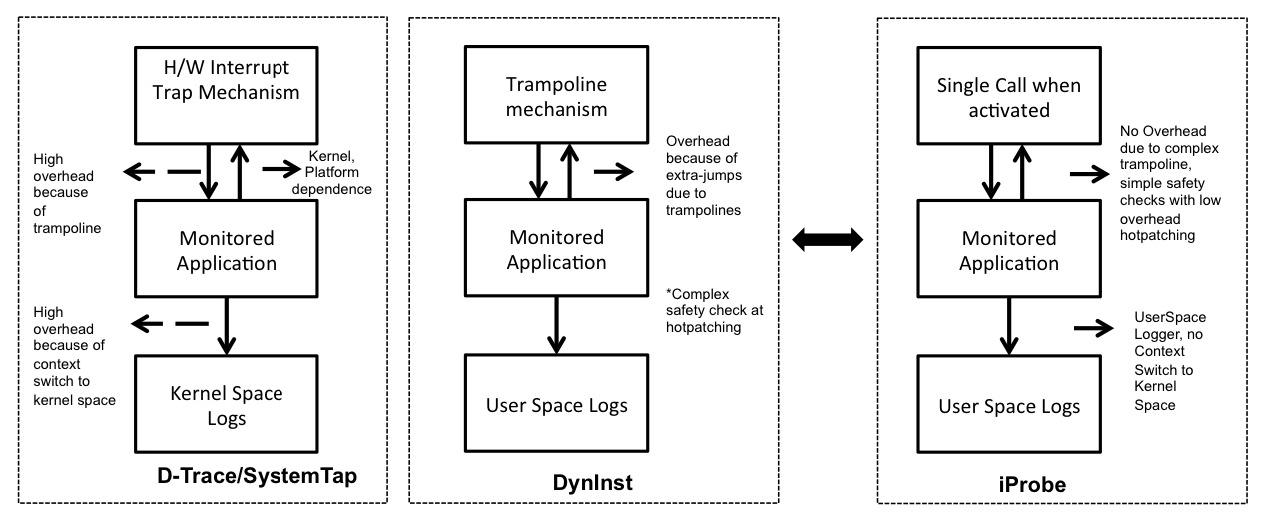
\includegraphics[width=0.9\textwidth]{iprobe/Images/related.eps}
		\caption{Advantages of iProbe over existing monitoring frameworks DTrace/SystemTap and DynInst}
		\label{fig:related}
	\end{center}
\end{figure*}

\subsection{Source Code or Compiler Instrumentation Mechanisms}
Source code instrumentation is one of the most widely available mechanisms for monitoring. 
In essence, users can insert debug statements with runtime flags to dump and inspect program status with varying verbosity levels. 
The log4j~\cite{log4j} and log4c~\cite{log4c} frameworks are commonly used libraries to perform program tracing in many open source projects in the source code level. 
Additionally compilers have several inbuilt profilers which can be used along with tools such as gprof and jprof to gather statistics about program execution.
While source code techniques allow very light weight instrumentation, by design they are static and can only be changed at the start of application execution. 
\iprobe on the other hand offers run-time instrumentation that allows dynamic decisions on tracing with comparable overhead.


\subsection{Run-time Instrumentation Mechanisms}
There are several kernel level tracing tools such as DTrace, LTTng, SystemTap \cite{dtrace,lttng,systemtap} developed by researchers over the years.
\iprobe differs from these approaches mainly in two ways: Firstly, all of these approaches use a technique similar to software interrupt to switch to kernel space and generate a log event by overwriting the target instructions. 
They then execute the instrumentation code, and either generate a trampoline mechanism or re-execute the overwritten target instructions and then jump back to the subsequent instructions. 
As shown in Figure.\ref{fig:related} this introduces context-switches between user-space and the kernel, causing needless overhead. 
iProbe avoids this overhead by having a completely user-space based design.
Secondly, all these approaches require to perform complex checks for correctness which can cause unnecessary overhead at both hotpatching, and when running an instrumented binary. 
%debug information at run-time to find the target function requested by the user. This requirement may not be met in production binaries, and iProbe does not require it in the binaries.

Fay \cite{fay} is a platform-dependent approach which uses the empty spaces at the start of the functions available in Windows binaries for instrumentation. 
To ensure the capture of the entry and exit of functions, Fay calls the target function within its instrumentation thereby introducing an extra stack frame for each target instrumentation. 
This operation is similar to a mini-trampoline and hence incurs an overhead. 
Fay logs function execution in the kernel space and hence also has a context-switch overhead.
\iprobe avoids such overhead by introducing markers at the beginning and end of
each function using a 

Another well known tool is DynInst\cite{dyninst}. This tool provides a rich dynamic instrumentation capability and has pure back box solution towards instrumentation of any application.
However, as shown in Figure.\ref{fig:related} it is also based on traditional trampoline mechanisms, and induces a high overhead because of unnecessary jump instructions.
Additionally it can have higher overhead because of complex security checks. 
Other similar trampoline based tools like \emph{kaho} and \emph{katana}\cite{katana,kaho} have also been proposed, but they focus more towards patching binaries to add \emph{fixes} to correct a bug.

% platform independent 
%compiler technique.

\subsection{Debuggers}
Instrumentation is a commonly used technique in debugging. Many debuggers such as gdb \cite{gdb} and Eclipse have breakpoints and watchpoints which can stop the execution of programs and inspect program conditions. These features are based on various techniques including \texttt{ptrace} and hardware debugging support (single step mode and debug registers). While they provide such powerful instrumentation capabilities, there are in general not adequate for beyond the debugging purposes due to overwhelming overhead.

\subsection{Dynamic Translation Tools}
Software engineering communities have been using dynamic translation tools such as Pin \cite{pin} and Valgrind \cite{valgrind} to inspect program characteristics. 
These tools dynamically translate program code before execution and allow users to insert custom instrumentation code flexibly. They are capable to instrument non-debug binaries and provide versatile tools such as memory checkers and program profilers. However, similar to debuggers, they are generally considered as debugging tools and their overhead is significantly higher than runtime tracers.




\part{Conclusions}
\chapter{Conclusions}
\label{ch:conclusions}

\section{Contributions}
\label{sec:contributions}

In this thesis, we have presented 

The main contributions of this thesis are as follows:

\begin{itemize}
	\item We are the first to present a new technique 
\end{itemize}

\section{Future Work}
\label{sec:future}

There are a number of interesting future work possibilities, both in the short term and further into the future.

In the future, we will explore: 
\begin{itemize}
	\item \textbf{Applications}: we aim to apply our system to real-time intrusion detection and statistical debugging.
	\item \textbf{Analysis}: we wish to define ``real-time'' data analysis techniques for traces and instrumentation done in \parikshan.
	\item \textbf{Optimize Live Cloning}: We plan to reduce the suspend time of live cloning, by utilizing several recent works in live migration.
\end{itemize}


\subsection{Immediate Future Work}
\label{sec:immediate}

\begin{itemize}
	\item Improve live cloning performance
\end{itemize}

\subsection{Possibilities for Long Term}
\label{sec:longterm}

\begin{itemize}
	\item Explore implementation in Virtual Machines
\end{itemize}

\section{Conclusion}
\label{sec:conclusion}

In this thesis we have explored approaches and frameworks for 

%%%
%%% Appendices
%%%
%\begin{comment}
\part{Appendices}
\appendix
\chapter{Active Debugging}
\label{sec:guided-approach}


\begin{figure}[!ht]
	\centering
	\includegraphics[width=0.25\textwidth]{guided/figs/offline.png}
	\label{fig:offlineDebugging}
	\caption{Debugging strategies for offline debugging}
\end{figure}


\section{Overview}

In this section, we introduce \activedebugging whereby developers can apply a patch/fix or apply a test in the \debugcontainer.
\activedebugging ensures that any modifications in the \debugcontainer does not lead to a state change in the \productioncontainer.
This will enable the debugger to fix/patch or run test-cases in the debug-container while ensuring forward progress and in sync with production. 
We are inspired from existing perpetual invivo testing frameworks like INVITE~\cite{invivo}(which also provides partial test-isolation), in the production environment.
We currently restrict \active debugging to patches/and test-cases only bring about local changes, and not global changes in the application.

\section{Description}

In Figure~\ref{fig:offlineDebugging}, we show the traditional mechanism of testing or validating patch/fixes in an application. 
In offline environments, developers apply patches and run the relevant inputs to verify that the patch works correctly. 
This is an interactive process, which allows one to verify the result and corrections before applying it to the production system.
Several cycles of this process is required, which may be followed by staged testing to ensure correctness before applying the update to the production.


\emph{Active Debugging} (see figure~\ref{fig:active-debugging}) allows debuggers to apply fixes, modify binaries and apply hotpatches to applications. 
The main idea is to do a fork/exec, or parallel execution of an unmodified application.
The unmodified binary continues execution without any change in the input.
The debug-container should ideally mimic the behavior of the production, so as to allow for forward progress in the application as the debug-container will receive the same input as production.
The target process will be forked at the call of the testing function, the forked process can then be tested, the input can be transformed, or alternatively the same input can be used to validate any test-condition. 
At the end of the execution the test-process output can be checked and killed. 
The advantage of this technique is that any tests/fixes can be validated in the run-time environment itself.
This reduces the time to fix and resolve the error. 
The tests and fixes should have a local impact and should not be allowed to continue 


\begin{figure}[!ht]
	\centering
	\includegraphics[width=0.75\textwidth]{guided/figs/active-debugging.png}
	\label{fig:active-debugging}
	\caption{Debugging Strategies for Active Debugging}
\end{figure}

For Java programs, since there is no “fork”, we can utilize a JNI call to a simple native C program which executes the fork. 
Performing a fork creates a copy-on-write version of the original process, so that the process running the unit test has its own writable memory area and cannot affect the in-process memory of the original. 
Once the test is invoked, the application can continue its normal execution, while the unit test runs in the other process. 
Note that the application and the unit test run in parallel in two processes; the test does not block normal operation of the application after the fork is performed.

The fork-exec design of test-isolation ensures that the ``in-process'' memory of the process execution is effectively isolated. 
The production/debug containers are completely isolated hence the test does not impact the production in any way. 
To ensure further isolation, we can allow the test fork to only call wrapper libraries which allow write operations in a cloned cow filesystem.
This can be done using a COW supported file-system with cloning functionality which are supported in ZFS and BTRFS.
For instance BTRFS provides a clone operation that atomically creates a copy-on-write snapshot of a file. By cloning the file system does not create a new link pointing to an existing inode; instead it creates a new inode that initially shares the same disk blocks with the original file. As a result cloning works only within the boundaries of the same BTRFS file system, and modifications to any of the cloned files are not visible to the original file and vice versa. 
This will of-course mean that we will constrain the debug/production environment to the File System of our choice.
All test-cases in the debug-container share the test file system.

%\chapter{List of Bugs used in Parikshan}

\section{Overview}

In order to show the feasibility of network replay to trigger the bug, we used several real-world bug-cases, and re-created them. In this appendix, we go through each of the bug-case and explain the re-creation mechanism.

The table~\ref{tab:appendix-casestudy} shows the lists of all the bugs studied for \parikshan.

\begin{table*}[ht]
	\centering
	\footnotesize
	
	\setlength{\tabcolsep}{2pt}
	\resizebox{\textwidth}{!}{
		\begin{tabular}{@{}c c c p{5.15cm} c c p{4.5cm}@{}}
			\toprule
			\textbf{Bug Type} & \textbf{Bug ID} & \textbf{Application} & \textbf{Symptom/Cause} & \textbf{\begin{tabular}[c]{@{}c@{}}Determ-\\ inistic\end{tabular}} & \textbf{Crash} & \multicolumn{1}{c}{\textbf{Trigger}} \\ \midrule
			\multirow{3}{*}{\textbf{Performance}} & MySQL \#15811 & mysql-5.0.15  & Bug caused due to multiple calls in a loop& Yes & No & Repeated insert into table \\ %\cmidrule(l){2-7} 
			& MySQL \#26527 & mysql-5.1.14 & Load data is slow in a partitioned table& Yes & No & Create table with partition and load data \\ %\cmidrule(l){2-7} 
			& MySQL \#49491 & mysql-5.1.38 & calculation of hash values inefficient & Yes & No & MySql client select requests \\ \midrule
			\multirow{5}{*}{\textbf{Concurrency}} & Apache \#25520 & httpd-2.0.4 & Per-child buffer management not thread safe & No & No & Continuous concurrent requests \\ %\cmidrule(l){2-7} 
			&Apache \#21287 & \parbox{1.5cm}{\centering httpd-2.0.48, php-4.4.1} & Dangling pointer due to atomicity violation & No & Yes & Continuous  concurrent request \\ %\cmidrule(l){2-7} 
			& MySQL \#644 & mysql-4.1 & data-race leading to crash & No & Yes & Concurrent select queries \\ %\cmidrule(l){2-7} 
			& MySQL \#169 & mysql-3.23 & Race condition leading to out-of-order logging & No & No & Delete and insert requests \\ %\cmidrule(l){2-7} 
			& MySQL \#791 & mysql-4.0 & Race - visible in logging& No & No & Concurrent flush log and insert requests \\ \midrule
			\multirow{4}{*}{\textbf{Semantic}} & Redis \#487 & redis-2.6.14 & Keys* command duplicate or omits keys & Yes & No & Set keys to expire, execute specific reqs \\ %\cmidrule(l){2-7} 
			& Cassandra \#5225 & cassandra-1.5.2 & Missing columns from wide row & Yes & No & Fetch columns from cassandra \\ %\cmidrule(l){2-7} 
			& Cassandra \#1837 & cassandra-0.7.0 & Deleted columns become available after flush & Yes & No & Insert, delete, and flush columns \\ %\cmidrule(l){2-7} 
			& Redis \#761 & redis-2.6.0 & Crash with large integer input & Yes & Yes & Query for input of large integer \\ \midrule
			\multirow{2}{*}{\textbf{Resource Leak}} & Redis \#614 & redis-2.6.0 & Master + slave, not replicated correctly & Yes & No & Setup replication, push  and pop some elements \\ %\cmidrule(l){2-7} 
			& Redis \#417 & redis-2.4.9 & Memory leak in master & Yes & No & Concurrent key set requests \\ \midrule
			\multirow{2}{*}{\textbf{Configuration}} & Redis \#957 & redis-2.6.11 & Slave cannot sync with master & Yes & No & Load a very large DB \\ %\cmidrule(l){2-7} 
			& HDFS \#1904 & hdfs-0.23.0 & Create a directory in wrong location & Yes & No & Create new directory \\ \bottomrule
		\end{tabular}%
	}
	\caption{List of real-world production bugs studied with \parikshan}
	\label{tab:appendix-casestudy}
\end{table*}


\section{Performance Bugs}

Performance bugs are bugs that result in a slowdown of the application. They are usually the result of algorithmic problem, which causes network retries or recursive execution, which could have been easily avoided or optimized.


%\end{comment}

%%%
%%% Bibliography
%%%
\part{Bibliography}
\addcontentsline{toc}{chapter}{Bibliography}
\bibliography{refs}
\bibliographystyle{named} 

\end{document}
